\documentclass[]{book}
\usepackage{lmodern}
\usepackage{amssymb,amsmath}
\usepackage{ifxetex,ifluatex}
\usepackage{fixltx2e} % provides \textsubscript
\ifnum 0\ifxetex 1\fi\ifluatex 1\fi=0 % if pdftex
  \usepackage[T1]{fontenc}
  \usepackage[utf8]{inputenc}
\else % if luatex or xelatex
  \ifxetex
    \usepackage{mathspec}
  \else
    \usepackage{fontspec}
  \fi
  \defaultfontfeatures{Ligatures=TeX,Scale=MatchLowercase}
\fi
% use upquote if available, for straight quotes in verbatim environments
\IfFileExists{upquote.sty}{\usepackage{upquote}}{}
% use microtype if available
\IfFileExists{microtype.sty}{%
\usepackage{microtype}
\UseMicrotypeSet[protrusion]{basicmath} % disable protrusion for tt fonts
}{}
\usepackage[margin=1in]{geometry}
\usepackage{hyperref}
\hypersetup{unicode=true,
            pdftitle={Introduction to R for Natural Resource Scientists},
            pdfauthor={Ben Staton},
            pdfborder={0 0 0},
            breaklinks=true}
\urlstyle{same}  % don't use monospace font for urls
\usepackage{natbib}
\bibliographystyle{apalike}
\usepackage{color}
\usepackage{fancyvrb}
\newcommand{\VerbBar}{|}
\newcommand{\VERB}{\Verb[commandchars=\\\{\}]}
\DefineVerbatimEnvironment{Highlighting}{Verbatim}{commandchars=\\\{\}}
% Add ',fontsize=\small' for more characters per line
\usepackage{framed}
\definecolor{shadecolor}{RGB}{248,248,248}
\newenvironment{Shaded}{\begin{snugshade}}{\end{snugshade}}
\newcommand{\KeywordTok}[1]{\textcolor[rgb]{0.13,0.29,0.53}{\textbf{#1}}}
\newcommand{\DataTypeTok}[1]{\textcolor[rgb]{0.13,0.29,0.53}{#1}}
\newcommand{\DecValTok}[1]{\textcolor[rgb]{0.00,0.00,0.81}{#1}}
\newcommand{\BaseNTok}[1]{\textcolor[rgb]{0.00,0.00,0.81}{#1}}
\newcommand{\FloatTok}[1]{\textcolor[rgb]{0.00,0.00,0.81}{#1}}
\newcommand{\ConstantTok}[1]{\textcolor[rgb]{0.00,0.00,0.00}{#1}}
\newcommand{\CharTok}[1]{\textcolor[rgb]{0.31,0.60,0.02}{#1}}
\newcommand{\SpecialCharTok}[1]{\textcolor[rgb]{0.00,0.00,0.00}{#1}}
\newcommand{\StringTok}[1]{\textcolor[rgb]{0.31,0.60,0.02}{#1}}
\newcommand{\VerbatimStringTok}[1]{\textcolor[rgb]{0.31,0.60,0.02}{#1}}
\newcommand{\SpecialStringTok}[1]{\textcolor[rgb]{0.31,0.60,0.02}{#1}}
\newcommand{\ImportTok}[1]{#1}
\newcommand{\CommentTok}[1]{\textcolor[rgb]{0.56,0.35,0.01}{\textit{#1}}}
\newcommand{\DocumentationTok}[1]{\textcolor[rgb]{0.56,0.35,0.01}{\textbf{\textit{#1}}}}
\newcommand{\AnnotationTok}[1]{\textcolor[rgb]{0.56,0.35,0.01}{\textbf{\textit{#1}}}}
\newcommand{\CommentVarTok}[1]{\textcolor[rgb]{0.56,0.35,0.01}{\textbf{\textit{#1}}}}
\newcommand{\OtherTok}[1]{\textcolor[rgb]{0.56,0.35,0.01}{#1}}
\newcommand{\FunctionTok}[1]{\textcolor[rgb]{0.00,0.00,0.00}{#1}}
\newcommand{\VariableTok}[1]{\textcolor[rgb]{0.00,0.00,0.00}{#1}}
\newcommand{\ControlFlowTok}[1]{\textcolor[rgb]{0.13,0.29,0.53}{\textbf{#1}}}
\newcommand{\OperatorTok}[1]{\textcolor[rgb]{0.81,0.36,0.00}{\textbf{#1}}}
\newcommand{\BuiltInTok}[1]{#1}
\newcommand{\ExtensionTok}[1]{#1}
\newcommand{\PreprocessorTok}[1]{\textcolor[rgb]{0.56,0.35,0.01}{\textit{#1}}}
\newcommand{\AttributeTok}[1]{\textcolor[rgb]{0.77,0.63,0.00}{#1}}
\newcommand{\RegionMarkerTok}[1]{#1}
\newcommand{\InformationTok}[1]{\textcolor[rgb]{0.56,0.35,0.01}{\textbf{\textit{#1}}}}
\newcommand{\WarningTok}[1]{\textcolor[rgb]{0.56,0.35,0.01}{\textbf{\textit{#1}}}}
\newcommand{\AlertTok}[1]{\textcolor[rgb]{0.94,0.16,0.16}{#1}}
\newcommand{\ErrorTok}[1]{\textcolor[rgb]{0.64,0.00,0.00}{\textbf{#1}}}
\newcommand{\NormalTok}[1]{#1}
\usepackage{longtable,booktabs}
\usepackage{graphicx,grffile}
\makeatletter
\def\maxwidth{\ifdim\Gin@nat@width>\linewidth\linewidth\else\Gin@nat@width\fi}
\def\maxheight{\ifdim\Gin@nat@height>\textheight\textheight\else\Gin@nat@height\fi}
\makeatother
% Scale images if necessary, so that they will not overflow the page
% margins by default, and it is still possible to overwrite the defaults
% using explicit options in \includegraphics[width, height, ...]{}
\setkeys{Gin}{width=\maxwidth,height=\maxheight,keepaspectratio}
\IfFileExists{parskip.sty}{%
\usepackage{parskip}
}{% else
\setlength{\parindent}{0pt}
\setlength{\parskip}{6pt plus 2pt minus 1pt}
}
\setlength{\emergencystretch}{3em}  % prevent overfull lines
\providecommand{\tightlist}{%
  \setlength{\itemsep}{0pt}\setlength{\parskip}{0pt}}
\setcounter{secnumdepth}{5}
% Redefines (sub)paragraphs to behave more like sections
\ifx\paragraph\undefined\else
\let\oldparagraph\paragraph
\renewcommand{\paragraph}[1]{\oldparagraph{#1}\mbox{}}
\fi
\ifx\subparagraph\undefined\else
\let\oldsubparagraph\subparagraph
\renewcommand{\subparagraph}[1]{\oldsubparagraph{#1}\mbox{}}
\fi

%%% Use protect on footnotes to avoid problems with footnotes in titles
\let\rmarkdownfootnote\footnote%
\def\footnote{\protect\rmarkdownfootnote}

%%% Change title format to be more compact
\usepackage{titling}

% Create subtitle command for use in maketitle
\newcommand{\subtitle}[1]{
  \posttitle{
    \begin{center}\large#1\end{center}
    }
}

\setlength{\droptitle}{-2em}

  \title{Introduction to R for Natural Resource Scientists}
    \pretitle{\vspace{\droptitle}\centering\huge}
  \posttitle{\par}
    \author{Ben Staton}
    \preauthor{\centering\large\emph}
  \postauthor{\par}
      \predate{\centering\large\emph}
  \postdate{\par}
    \date{with contributions from Henry Hershey}

\usepackage{booktabs}
\usepackage{amsthm}
\makeatletter
\def\thm@space@setup{%
  \thm@preskip=8pt plus 2pt minus 4pt
  \thm@postskip=\thm@preskip
}
\makeatother

\usepackage{amsthm}
\newtheorem{theorem}{Theorem}[chapter]
\newtheorem{lemma}{Lemma}[chapter]
\theoremstyle{definition}
\newtheorem{definition}{Definition}[chapter]
\newtheorem{corollary}{Corollary}[chapter]
\newtheorem{proposition}{Proposition}[chapter]
\theoremstyle{definition}
\newtheorem{example}{Example}[chapter]
\theoremstyle{definition}
\newtheorem{exercise}{Exercise}[chapter]
\theoremstyle{remark}
\newtheorem*{remark}{Remark}
\newtheorem*{solution}{Solution}
\begin{document}
\maketitle

{
\setcounter{tocdepth}{1}
\tableofcontents
}
\chapter*{Overview}\label{overview}
\addcontentsline{toc}{chapter}{Overview}

This is intended to be a first course in R programming. It is by no
means comprehensive, but instead attempts to introduce the main topics
needed to get a beginner up and running with applying R to their own
work. There will be no prior knowledge assumed on the part of the
student regarding R or programming. In the later chapters, e.g.,
Chapters \ref{ch3} and \ref{ch4}, an understanding of statistics at the
introductory undergraduate level would be helpful.

\chapter{Introduction to the R Environment}\label{ch1}

\begin{center}\rule{0.5\linewidth}{\linethickness}\end{center}

\section*{Chapter Overview}\label{chapter-overview}
\addcontentsline{toc}{section}{Chapter Overview}

In this first chapter, you will get familiar with the basics of using R.
You will learn:

\begin{itemize}
\tightlist
\item
  the use of R as a basic calculator
\item
  some basic object types
\item
  some basic data classes
\item
  some basic data structures
\item
  how to read in data
\item
  how to write out data
\item
  how to write your own functions
\end{itemize}

\section*{Before You Begin: Install R and
RStudio}\label{before-you-begin-install-r-and-rstudio}
\addcontentsline{toc}{section}{Before You Begin: Install R and RStudio}

First off, you will need to get R and RStudio\footnote{While it is
  possible to run R on it's own, it rather clunky and you are strongly
  advised to use RStudio given its compactness, neat features, code
  tools (like syntax and parentheses highlighting). This workshop will
  assume you are using RStudio} onto your computer. Please see
\textbf{Appendix A} for details on installing these programs on your
operating system.

\section{The R Studio Interface}\label{the-r-studio-interface}

Once you open up R Studio for the first time, you will see three panes:
the left hand side is the \textbf{console} where results from executed
commands are printed, and the two panes on the right are for additional
information to help you code more efficiently - don't worry too much
about what these are at the moment. For now, focus your attention on the
console.

\subsection{Write Some Simple Code}\label{write-some-simple-code}

To start off, you will just use R as a calculator. Type these commands
(not the lines with \texttt{\#\#}, those are output\footnote{The
  formatting used here includes \texttt{\#\#} on output to denote code
  and output separately. You won't see the \texttt{\#\#} show up in your
  console.}) one at a time and hit \textbf{CTRL + ENTER} to run it. The
spaces don't matter at all, they are used here for clairity and for
styling.\footnote{To learn more about standard R code styling, check out
  Hadley Wickham's \href{http://adv-r.had.co.nz/Style.html}{great
  chapter} about it.}

\begin{Shaded}
\begin{Highlighting}[]
\DecValTok{3} \OperatorTok{+}\StringTok{ }\DecValTok{3}
\end{Highlighting}
\end{Shaded}

\begin{verbatim}
## [1] 6
\end{verbatim}

\begin{Shaded}
\begin{Highlighting}[]
\DecValTok{12}\OperatorTok{/}\DecValTok{4}
\end{Highlighting}
\end{Shaded}

\begin{verbatim}
## [1] 3
\end{verbatim}

Notice that when you run each line, it prints the command and the output
to the console.

R is an \textbf{object oriented language}, which means that you fill
objects with data do things with them. Make an object called \texttt{x}
that stores the result of the calculation \texttt{3\ +\ 3} (type this
and run using \textbf{CTRL + ENTER}):

\begin{Shaded}
\begin{Highlighting}[]
\NormalTok{x =}\StringTok{ }\DecValTok{3} \OperatorTok{+}\StringTok{ }\DecValTok{3}
\end{Highlighting}
\end{Shaded}

Notice that running this line did not return a value as before. This is
because in that line you are \textbf{assigning} a value to the object
\texttt{x}. You can view the contents of \texttt{x} by typing its name
alone and running just that:

\begin{Shaded}
\begin{Highlighting}[]
\NormalTok{x}
\end{Highlighting}
\end{Shaded}

\begin{verbatim}
## [1] 6
\end{verbatim}

When used this way, the \texttt{=} sign denotes assignment of the value
on the right-hand side to an object with the name on the left-hand side.
The \texttt{\textless{}-} serves this same purpose so in this context
the two are interchangable:

\begin{Shaded}
\begin{Highlighting}[]
\NormalTok{y <-}\StringTok{ }\DecValTok{2} \OperatorTok{+}\StringTok{ }\DecValTok{5}
\end{Highlighting}
\end{Shaded}

You can highlight smaller sections of a line to run as well. For example
after creating \texttt{y} above, press the \textbf{up arrow} to see the
line you just ran, highlight just the \texttt{y}, and press \textbf{CTRL
+ ENTER}. From this point forward, the verb ``run'' means execute some
code using \textbf{CTRL + ENTER}.

You can use your objects together to make a new object:

\begin{Shaded}
\begin{Highlighting}[]
\NormalTok{z =}\StringTok{ }\NormalTok{y }\OperatorTok{-}\StringTok{ }\NormalTok{x}
\end{Highlighting}
\end{Shaded}

\section{Saving Your Code: Scripts}\label{scripts}

If you closed R at this moment, your work would be lost. Running code in
the console like you have just done \textbf{does not save a record of
your work}. To save R code, you must use what is called a
\textbf{script}, which is a plain-text file with the extension
\texttt{.R}. To create a new script file, go to \emph{File
\textgreater{} New File \textgreater{} R Script}, or use the keyboard
shortcut \textbf{CTRL + SHIFT + N}. A new pane will open called the
\textbf{source} pane - this is where you will edit your code and save
your progress. R Scripts are a key feature of reproducible research with
R, given that if they are well-written they can present a complete
roadmap of your statistical analysis and workflow.

\section{The Working Directory}\label{working-dir}

You will want to save your hard work. A key part of doing saving your
work is thinking about \textbf{where} you save it. In R, a key concept
is the \textbf{working directory}. This is the location (i.e., folder)
on your computer where your current R session will ``talk to'' by
default. The working directory is where R will read files from and write
files to by default, and is where all of your data should be stored for
your analysis in R. Because you'll likely be visiting it often, it
should probably be somewhere that is easy to remember and not too deeply
buried in your computer's file system.

Save your script somewhere like
\texttt{C:/Users/YOU/Documents/R-Workshop/Chapter1} on your computer. To
set the working directory to this location, you have three options:

\begin{enumerate}
\def\labelenumi{\arabic{enumi}.}
\item
  \textbf{Go to Session \textgreater{} Set Working Directory
  \textgreater{} Source File Location}. This will set the working
  directory to the location of the file that is currently open in your
  source pane.
\item
  \textbf{Go to Session \textgreater{} Set Working Directory
  \textgreater{} Choose Directory}. This will open an interactive file
  selection window to allow you to navigate to the desired directory.
\item
  \textbf{Use code}. In the console, you can type
  \texttt{setwd("C:/Users/YOU/Documents/R-Workshop/Chapter1")}. If at
  any point you want to know where your current working directory is set
  to, you can either look at the top of the console pane, which shows
  the full path or by running \texttt{getwd()} in the console.
\end{enumerate}

\textbf{The main benefits of using a working directory are}:

\begin{itemize}
\tightlist
\item
  Files are read from and written to a consistent and predictable place
  everytime
\item
  Everything for your analysis is organized into one place
\item
  You don't have to continously type file paths to your work. If
  \texttt{file.txt} is a file in your current working directory, you can
  reference it your R session using \texttt{"file.txt"} rather than with
  \texttt{"C:/Users/YOU/Documents/R-Workshop/Chapter1/file.txt"} each
  time.
\end{itemize}

\section{R Object Types}\label{r-object-types}

R has a variety of object types that you will need to become familiar
with.

\subsection{Functions}\label{functions}

Much of your work in R will involve functions. A function is called
using the syntax:

\begin{Shaded}
\begin{Highlighting}[]
\KeywordTok{fun}\NormalTok{(}\DataTypeTok{arg1 =}\NormalTok{ value1, }\DataTypeTok{arg2 =}\NormalTok{ value2)}
\end{Highlighting}
\end{Shaded}

Here, \texttt{fun} is the \textbf{function name} and \texttt{arg1} and
\texttt{arg2} are called \textbf{arguments}. Functions take input in the
form of the arguments, do some task with them, then return some output.
The parentheses are a sure sign that \texttt{fun} is a function.

We have passed the function two arguments by name: all functions have
arguments, all arguments have names, and there is always a default order
to the arguments. If you memorize the argument order of functions you
use frequently, you don't have to specify the argument name:

\begin{Shaded}
\begin{Highlighting}[]
\KeywordTok{fun}\NormalTok{(value1, value2)}
\end{Highlighting}
\end{Shaded}

would give the same result as the command above in which the argument
names were specified.

Here's a real example:

\begin{Shaded}
\begin{Highlighting}[]
\KeywordTok{print}\NormalTok{(}\DataTypeTok{x =}\NormalTok{ z)}
\end{Highlighting}
\end{Shaded}

\begin{verbatim}
## [1] 1
\end{verbatim}

The function is \texttt{print}, the argument is \texttt{x}, and the
value we have supplied the argument is the object \texttt{z}. The task
that \texttt{print} does is to print the value of \texttt{z} to the
console.

R has lots of built-in information to help you learn how to use a
function. Take a look at the help file for the mean function. Run
\texttt{?mean} in the console: a window on the right-hand side of the R
Studio interface should open. The help file tells you what goes into a
function and what comes out. For more complex functions it also tells
you what all of the options (i.e., arguments) can do. Help files can be
a bit intimidating to interpret at first, but they are all organized the
same and once you learn their layout you will know where to go to find
the information you're looking for.

\subsection{Vectors}\label{vectors}

Vectors are one of the most common data structures. A vector is a set of
numbers going in only one dimension. Each position in a vector is termed
an \textbf{element}, and the number of elements is termed the
\textbf{length} of the vector. Here are some ways to make some vectors
with different elements, all of length five:

\begin{Shaded}
\begin{Highlighting}[]
\CommentTok{# this is a comment. R will ignore all text on a line after a #}
\CommentTok{# the ; means run everything after it on a new line}

\CommentTok{# count up by 1}
\NormalTok{month =}\StringTok{ }\DecValTok{2}\OperatorTok{:}\DecValTok{6}\NormalTok{; month}
\end{Highlighting}
\end{Shaded}

\begin{verbatim}
## [1] 2 3 4 5 6
\end{verbatim}

\begin{Shaded}
\begin{Highlighting}[]
\CommentTok{# count up by 2}
\NormalTok{day =}\StringTok{ }\KeywordTok{seq}\NormalTok{(}\DataTypeTok{from =} \DecValTok{1}\NormalTok{, }\DataTypeTok{to =} \DecValTok{9}\NormalTok{, }\DataTypeTok{by =} \DecValTok{2}\NormalTok{); day}
\end{Highlighting}
\end{Shaded}

\begin{verbatim}
## [1] 1 3 5 7 9
\end{verbatim}

\begin{Shaded}
\begin{Highlighting}[]
\CommentTok{# repeat the same number (repeat 2018 5 times)}
\NormalTok{year =}\StringTok{ }\KeywordTok{rep}\NormalTok{(}\DecValTok{2018}\NormalTok{, }\DecValTok{5}\NormalTok{); year}
\end{Highlighting}
\end{Shaded}

\begin{verbatim}
## [1] 2018 2018 2018 2018 2018
\end{verbatim}

The \texttt{{[}1{]}} that shows up is a element position, more on this
later (see Section \ref{sub}). If you wish to know how many elements are
in a vector, use \texttt{length}:

\begin{Shaded}
\begin{Highlighting}[]
\KeywordTok{length}\NormalTok{(year)}
\end{Highlighting}
\end{Shaded}

\begin{verbatim}
## [1] 5
\end{verbatim}

You can also create a vector ``by-hand'' using the \texttt{c}
function\footnote{The \texttt{c} stands for \textbf{concatenate}, which
  basically means combine many smaller objects into one larger object}:

\begin{Shaded}
\begin{Highlighting}[]
\CommentTok{# a numeric vector}
\NormalTok{number =}\StringTok{ }\KeywordTok{c}\NormalTok{(}\DecValTok{4}\NormalTok{, }\DecValTok{7}\NormalTok{, }\DecValTok{8}\NormalTok{, }\DecValTok{10}\NormalTok{, }\DecValTok{15}\NormalTok{); number}
\end{Highlighting}
\end{Shaded}

\begin{verbatim}
## [1]  4  7  8 10 15
\end{verbatim}

\begin{Shaded}
\begin{Highlighting}[]
\CommentTok{# a character vector}
\NormalTok{pond =}\StringTok{ }\KeywordTok{c}\NormalTok{(}\StringTok{"F11"}\NormalTok{, }\StringTok{"S28"}\NormalTok{, }\StringTok{"S30"}\NormalTok{, }\StringTok{"S8"}\NormalTok{, }\StringTok{'S11'}\NormalTok{); pond}
\end{Highlighting}
\end{Shaded}

\begin{verbatim}
## [1] "F11" "S28" "S30" "S8"  "S11"
\end{verbatim}

Note the difference between the numeric and character vectors. The the
terms ``numeric'' and ``character''" represent \textbf{data classes},
which specify the type of data the vector is holding:

\begin{itemize}
\tightlist
\item
  A \textbf{numeric vector} stores numbers. You can do math with numeric
  vectors
\item
  A \textbf{character vector} stores what are essentially letters. You
  can't do math with letters. A character vector is easy to spot because
  the elements will be wrapped with quotes\footnote{\texttt{"\ "} or
    \texttt{\textquotesingle{}\ \textquotesingle{}} both work as long as
    you use the same on the front and end of the element}.
\end{itemize}

A vector can only hold one data class at a time:

\begin{Shaded}
\begin{Highlighting}[]
\NormalTok{v =}\StringTok{ }\KeywordTok{c}\NormalTok{(}\DecValTok{1}\NormalTok{,}\DecValTok{2}\NormalTok{,}\DecValTok{3}\NormalTok{,}\StringTok{"a"}\NormalTok{); v}
\end{Highlighting}
\end{Shaded}

\begin{verbatim}
## [1] "1" "2" "3" "a"
\end{verbatim}

Notice how all the elements now have quotes around them. The numbers
have been \textbf{coerced} to characters\footnote{The coersion works
  this way because numbers can be expressed as characters, but a letter
  cannot be unambiguously be expressed as a number.}. If we attempted to
calculate the sum of our vector:

\begin{Shaded}
\begin{Highlighting}[]
\KeywordTok{sum}\NormalTok{(v)}
\end{Highlighting}
\end{Shaded}

\begin{verbatim}
## Error in sum(v): invalid 'type' (character) of argument
\end{verbatim}

we would find that it is impossible in its current form.

\subsection{Matrices}\label{matrices}

Matrices act just like vectors, but they are in two dimensions, i.e.,
they have both rows and columns. One easy way to make a matrix is by
combining vectors you have already made:

\begin{Shaded}
\begin{Highlighting}[]
\CommentTok{# combine vectors by column (each vector will become a column)}
\NormalTok{m1 =}\StringTok{ }\KeywordTok{cbind}\NormalTok{(month, day, year, number); m1}
\end{Highlighting}
\end{Shaded}

\begin{verbatim}
##      month day year number
## [1,]     2   1 2018      4
## [2,]     3   3 2018      7
## [3,]     4   5 2018      8
## [4,]     5   7 2018     10
## [5,]     6   9 2018     15
\end{verbatim}

\begin{Shaded}
\begin{Highlighting}[]
\CommentTok{# combine vectors by row (each vector will become a row)}
\NormalTok{m2 =}\StringTok{ }\KeywordTok{rbind}\NormalTok{(month, day, year, number); m2}
\end{Highlighting}
\end{Shaded}

\begin{verbatim}
##        [,1] [,2] [,3] [,4] [,5]
## month     2    3    4    5    6
## day       1    3    5    7    9
## year   2018 2018 2018 2018 2018
## number    4    7    8   10   15
\end{verbatim}

Just like vectors, matrices can hold only one data class (note the
coersion of numbers to characters):

\begin{Shaded}
\begin{Highlighting}[]
\KeywordTok{cbind}\NormalTok{(m1, pond)}
\end{Highlighting}
\end{Shaded}

\begin{verbatim}
##      month day year   number pond 
## [1,] "2"   "1" "2018" "4"    "F11"
## [2,] "3"   "3" "2018" "7"    "S28"
## [3,] "4"   "5" "2018" "8"    "S30"
## [4,] "5"   "7" "2018" "10"   "S8" 
## [5,] "6"   "9" "2018" "15"   "S11"
\end{verbatim}

\subsection{Data Frames}\label{data-frames}

Many data sets you will work with require storing different data classes
in different columns, which would rule out the use of a matrix. This is
where \textbf{data frames} come in:

\begin{Shaded}
\begin{Highlighting}[]
\NormalTok{df1 =}\StringTok{ }\KeywordTok{data.frame}\NormalTok{(month, day, year, number, pond); df1}
\end{Highlighting}
\end{Shaded}

\begin{verbatim}
##   month day year number pond
## 1     2   1 2018      4  F11
## 2     3   3 2018      7  S28
## 3     4   5 2018      8  S30
## 4     5   7 2018     10   S8
## 5     6   9 2018     15  S11
\end{verbatim}

Notice the lack of quotation marks which indicates that all variables
(i.e., columns) are stored as their original data class.

It is important to know what kind of object type you are using, since R
treats them differently. For example, some functions can only use a
certain object type. The same holds true for data classes (numeric
vs.~character).You can quickly determine what kind of object you are
dealing with by using the \texttt{class} function. Simply run
\texttt{class(object.name)}:

\begin{Shaded}
\begin{Highlighting}[]
\KeywordTok{class}\NormalTok{(day); }\KeywordTok{class}\NormalTok{(pond); }\KeywordTok{class}\NormalTok{(m1); }\KeywordTok{class}\NormalTok{(df1)}
\end{Highlighting}
\end{Shaded}

\begin{verbatim}
## [1] "numeric"
\end{verbatim}

\begin{verbatim}
## [1] "character"
\end{verbatim}

\begin{verbatim}
## [1] "matrix"
\end{verbatim}

\begin{verbatim}
## [1] "data.frame"
\end{verbatim}

\section{Factors}\label{factors}

At this point, it is worthwhile to introduce an additional data class:
factors. Notice the class of the \texttt{pond} variable in \texttt{df1}:

\begin{Shaded}
\begin{Highlighting}[]
\KeywordTok{class}\NormalTok{(df1}\OperatorTok{$}\NormalTok{pond)}
\end{Highlighting}
\end{Shaded}

\begin{verbatim}
## [1] "factor"
\end{verbatim}

The character vector \texttt{pond} was coerced to a factor when you
placed it in the data frame. A vector with a \textbf{factor} class is
like a character vector in that you see letters and that you can't do
math on it. However, a factor has additional properties: in particular,
it is a grouping variable. See what happens when you print the
\texttt{pond} variable:

\begin{Shaded}
\begin{Highlighting}[]
\NormalTok{df1}\OperatorTok{$}\NormalTok{pond}
\end{Highlighting}
\end{Shaded}

\begin{verbatim}
## [1] F11 S28 S30 S8  S11
## Levels: F11 S11 S28 S30 S8
\end{verbatim}

That looks weird, huh? A factor has levels, with each level being a
subcategory of the factor. You can see the unique levels of your factor
by running:

\begin{Shaded}
\begin{Highlighting}[]
\KeywordTok{levels}\NormalTok{(df1}\OperatorTok{$}\NormalTok{pond)}
\end{Highlighting}
\end{Shaded}

\begin{verbatim}
## [1] "F11" "S11" "S28" "S30" "S8"
\end{verbatim}

Additionally, factor levels have an assigned order (even if the levels
are totally nominal), which will become important in Chapter \ref{ch3}
when you learn how to fit linear models to groups of data, in which one
level is the ``reference'' group that all other groups are compared to.

If you're running into errors about R expecting character vectors, it
may be because they are actually stored as factors. When you make a data
frame, you'll often have the option to turn off the automatic factor
coersion. For example:

\begin{Shaded}
\begin{Highlighting}[]
\KeywordTok{data.frame}\NormalTok{(month, day, year, number, pond, }\DataTypeTok{stringsAsFactors =}\NormalTok{ F)}
\KeywordTok{read.csv}\NormalTok{(}\StringTok{"streams.csv"}\NormalTok{, }\DataTypeTok{stringsAsFactors =}\NormalTok{ F)  }\CommentTok{# see below for details on read.csv}
\end{Highlighting}
\end{Shaded}

will result in character vectors remaining that way as opposed to being
coerced to factors. This can be preferable if you are doing many string
manipulations, as character vectors are often easier to work with than
factors.

\section{Vector Math}\label{vector-math}

R does vectorized calculations. This means that if supplied with two
numeric vectors of equal length and a mathematical operator, R will
perform the calculation on each pair of elements. For example, if you
wanted to add the two vectors vector \texttt{day} and \texttt{month},
then you would just run:

\begin{Shaded}
\begin{Highlighting}[]
\NormalTok{dm =}\StringTok{ }\NormalTok{day }\OperatorTok{+}\StringTok{ }\NormalTok{month; dm}
\end{Highlighting}
\end{Shaded}

\begin{verbatim}
## [1]  3  6  9 12 15
\end{verbatim}

You typically should ensure that the vectors you are doing math with are
of equal lengths.

You could do the same calculation to each element (e.g., divide each
element by 2) with:

\begin{Shaded}
\begin{Highlighting}[]
\NormalTok{dm}\OperatorTok{/}\DecValTok{2}
\end{Highlighting}
\end{Shaded}

\begin{verbatim}
## [1] 1.5 3.0 4.5 6.0 7.5
\end{verbatim}

\section{Data Queries/Subsets/Retrievals}\label{sub}

This perhaps the most important and versatile skills to know in R. So
you have an object with data in it and you want to use it for analysis.
But you don't want the whole dataset. You want to use just a few rows or
just a few columns, or perhaps you need just a single element from a
vector. This section is devoted to ways you can extract certain parts of
a data object (the terms \textbf{query} and \textbf{subset} are often
used interchangeably to describe this task). There are three main
methods:

\begin{enumerate}
\def\labelenumi{\arabic{enumi}.}
\tightlist
\item
  \textbf{By Index} -- This method allows you to pull out specific
  rows/columns by their location in an object. However, you must know
  exactly where in the object the desired data are. An \textbf{index} is
  a location of a element in a data object, like the element position or
  the position of a specific row or column. To subset by index, you
  specify the object, then what rows, then what columns. The syntax for
  subsetting a vector by index is \texttt{vector{[}element{]}} and for a
  matrix it is \texttt{matrix{[}row,column{]}}. Here are some examples
\end{enumerate}

\begin{Shaded}
\begin{Highlighting}[]
\CommentTok{# show all of day, then subset the third element}
\NormalTok{day; day[}\DecValTok{3}\NormalTok{]}
\end{Highlighting}
\end{Shaded}

\begin{verbatim}
## [1] 1 3 5 7 9
\end{verbatim}

\begin{verbatim}
## [1] 5
\end{verbatim}

\begin{Shaded}
\begin{Highlighting}[]
\CommentTok{# show all of m1, then subset the cell in row 1 col 3 }
\NormalTok{m1; m1[}\DecValTok{1}\NormalTok{,}\DecValTok{3}\NormalTok{]}
\end{Highlighting}
\end{Shaded}

\begin{verbatim}
##      month day year number
## [1,]     2   1 2018      4
## [2,]     3   3 2018      7
## [3,]     4   5 2018      8
## [4,]     5   7 2018     10
## [5,]     6   9 2018     15
\end{verbatim}

\begin{verbatim}
## year 
## 2018
\end{verbatim}

\begin{Shaded}
\begin{Highlighting}[]
\CommentTok{# show all of df1, then subset the entire first column}
\NormalTok{df1; df1[,}\DecValTok{1}\NormalTok{]}
\end{Highlighting}
\end{Shaded}

\begin{verbatim}
##   month day year number pond
## 1     2   1 2018      4  F11
## 2     3   3 2018      7  S28
## 3     4   5 2018      8  S30
## 4     5   7 2018     10   S8
## 5     6   9 2018     15  S11
\end{verbatim}

\begin{verbatim}
## [1] 2 3 4 5 6
\end{verbatim}

Note this last line: the \texttt{{[},1{]}} says ``keep all the rows, but
take only the first column''.

Here is another example:

\begin{Shaded}
\begin{Highlighting}[]
\CommentTok{# show m1, then subset the 1st, 2nd, and 4th rows and every column}
\NormalTok{m1; m1[}\KeywordTok{c}\NormalTok{(}\DecValTok{1}\NormalTok{,}\DecValTok{2}\NormalTok{,}\DecValTok{4}\NormalTok{),]}
\end{Highlighting}
\end{Shaded}

\begin{verbatim}
##      month day year number
## [1,]     2   1 2018      4
## [2,]     3   3 2018      7
## [3,]     4   5 2018      8
## [4,]     5   7 2018     10
## [5,]     6   9 2018     15
\end{verbatim}

\begin{verbatim}
##      month day year number
## [1,]     2   1 2018      4
## [2,]     3   3 2018      7
## [3,]     5   7 2018     10
\end{verbatim}

Notice how you can pass a vector of row indices here to exclude the
3\textsuperscript{rd} and 5\textsuperscript{th} rows.

\textbf{2. By name} -- This method allows you to pull out a specific
column of data based on what the column name is. Of course, the column
must have a name first. The name method uses the \texttt{\$} operator:

\begin{Shaded}
\begin{Highlighting}[]
\NormalTok{df1}\OperatorTok{$}\NormalTok{month}
\end{Highlighting}
\end{Shaded}

\begin{verbatim}
## [1] 2 3 4 5 6
\end{verbatim}

You can combine these two methods:

\begin{Shaded}
\begin{Highlighting}[]
\NormalTok{df1}\OperatorTok{$}\NormalTok{month[}\DecValTok{3}\NormalTok{]}
\end{Highlighting}
\end{Shaded}

\begin{verbatim}
## [1] 4
\end{verbatim}

\begin{Shaded}
\begin{Highlighting}[]
\CommentTok{# or}
\NormalTok{df1[,}\StringTok{"year"}\NormalTok{]}
\end{Highlighting}
\end{Shaded}

\begin{verbatim}
## [1] 2018 2018 2018 2018 2018
\end{verbatim}

The by name (\texttt{\$}) method is useful because it can be used to add
columns to a data frame:

\begin{Shaded}
\begin{Highlighting}[]
\NormalTok{df1}\OperatorTok{$}\NormalTok{dm =}\StringTok{ }\NormalTok{df1}\OperatorTok{$}\NormalTok{day }\OperatorTok{+}\StringTok{ }\NormalTok{df1}\OperatorTok{$}\NormalTok{month; df1}
\end{Highlighting}
\end{Shaded}

\begin{verbatim}
##   month day year number pond dm
## 1     2   1 2018      4  F11  3
## 2     3   3 2018      7  S28  6
## 3     4   5 2018      8  S30  9
## 4     5   7 2018     10   S8 12
## 5     6   9 2018     15  S11 15
\end{verbatim}

\begin{enumerate}
\def\labelenumi{\arabic{enumi}.}
\setcounter{enumi}{2}
\tightlist
\item
  \textbf{Logical Subsetting} -- This is perhaps the most flexible
  method, and is described in Section \ref{logsub}.
\end{enumerate}

\section*{EXERCISE 1A}\label{exercise-1a}
\addcontentsline{toc}{section}{EXERCISE 1A}

Take a break to apply what you've learned so far. In this exercise,
you'll be using what you learned about creating objects and the
differences between different data classes. You will be entering this
data frame into R by hand and doing some basic data subsets.

\begin{longtable}[]{@{}cccc@{}}
\toprule
\begin{minipage}[b]{0.11\columnwidth}\centering\strut
Lake\strut
\end{minipage} & \begin{minipage}[b]{0.09\columnwidth}\centering\strut
Area\strut
\end{minipage} & \begin{minipage}[b]{0.09\columnwidth}\centering\strut
Time\strut
\end{minipage} & \begin{minipage}[b]{0.09\columnwidth}\centering\strut
Fish\strut
\end{minipage}\tabularnewline
\midrule
\endhead
\begin{minipage}[t]{0.11\columnwidth}\centering\strut
Big\strut
\end{minipage} & \begin{minipage}[t]{0.09\columnwidth}\centering\strut
100\strut
\end{minipage} & \begin{minipage}[t]{0.09\columnwidth}\centering\strut
1000\strut
\end{minipage} & \begin{minipage}[t]{0.09\columnwidth}\centering\strut
643\strut
\end{minipage}\tabularnewline
\begin{minipage}[t]{0.11\columnwidth}\centering\strut
Small\strut
\end{minipage} & \begin{minipage}[t]{0.09\columnwidth}\centering\strut
25\strut
\end{minipage} & \begin{minipage}[t]{0.09\columnwidth}\centering\strut
1200\strut
\end{minipage} & \begin{minipage}[t]{0.09\columnwidth}\centering\strut
203\strut
\end{minipage}\tabularnewline
\begin{minipage}[t]{0.11\columnwidth}\centering\strut
Square\strut
\end{minipage} & \begin{minipage}[t]{0.09\columnwidth}\centering\strut
45\strut
\end{minipage} & \begin{minipage}[t]{0.09\columnwidth}\centering\strut
1400\strut
\end{minipage} & \begin{minipage}[t]{0.09\columnwidth}\centering\strut
109\strut
\end{minipage}\tabularnewline
\begin{minipage}[t]{0.11\columnwidth}\centering\strut
Circle\strut
\end{minipage} & \begin{minipage}[t]{0.09\columnwidth}\centering\strut
30\strut
\end{minipage} & \begin{minipage}[t]{0.09\columnwidth}\centering\strut
1600\strut
\end{minipage} & \begin{minipage}[t]{0.09\columnwidth}\centering\strut
15\strut
\end{minipage}\tabularnewline
\bottomrule
\end{longtable}

\begin{enumerate}
\def\labelenumi{\arabic{enumi}.}
\item
  Create a new file called \texttt{Ex\_1A.R}. Set the working directory
  to the folder containing \texttt{Ex\_1A.R}.
\item
  Enter these data into vectors. Call the vectors whatever you would
  like. Should you enter the data as vectors by rows, or by columns?
  (\emph{Hint: remember the properties of vectors}).
\item
  Combine your vectors into a data frame. Why should you use a data
  frame instead of a matrix?
\item
  Subset all of the data from Small Lake.
\item
  Subset the area for all of the lakes.
\item
  Subset the number of fish for Big and Square lakes.
\item
  You realize that you sampled 209 fish at Square Lake, not 109. Fix the
  mistake. There are two ways to do this, can you think of them both?
  Which do you think is better?
\item
  Save your script. Close R and re-open your script to see that it was
  saved.
\end{enumerate}

\section{Read External Data Files}\label{read}

It is rare that you will enter data by hand as you did in Exercise 1A.
Often, you have a dataset that you wish to analyze or manipulate. R has
several ways to read information from data files and in this workshop,
we will be using a common and simple method: reading in \texttt{.csv}
files. \texttt{.csv} files are data files that separate columns with
commas\footnote{Note that if your computer is configured for a
  Spanish-speaking country, Microsoft Excel might convert decimals to
  commas. This can really mess with reading in data - I would suggest
  changing the language of Excel if you find this to be the case.}. If
your data are in a Microsoft Excel spreadsheet, you can save your
spreadsheet file as a CSV file (\emph{File \textgreater{} Save As
\textgreater{} Save as Type\textgreater{} CSV (Comma Delimited)}).
Several dialog boxes will open asking if you are sure you want to save
it as a \texttt{.csv} file.

The syntax for reading in a \texttt{.csv} file is:

\begin{Shaded}
\begin{Highlighting}[]
\NormalTok{dat =}\StringTok{ }\KeywordTok{read.csv}\NormalTok{(}\StringTok{"FileName.csv"}\NormalTok{)}
\end{Highlighting}
\end{Shaded}

The data files for this workshop are found in the GitHub repository:
\url{https://github.com/bstaton1/au-r-workshop-data/tree/master}.
Navigate to this repository, find the file called \texttt{streams.csv},
download that file\footnote{To download a single file from GitHub, click
  on the file, then click ``Raw'' in the toolbar on the topright, then
  right-click anywhere in the document and click ``Save As\ldots{}''.
  You can also download a zip folder with all of the \texttt{.csv}
  files, go to ``Clone or Download''}, and place it in your working
directory for this session. This document assumes your working directory
is \texttt{C:/Users/YOU/Documents/R-Workshop/Chapter1}, though the one
you are actually using may be slightly different. We can read the
contents of \texttt{streams.csv} into R using this code (ensure your
working directory is set first):

\begin{Shaded}
\begin{Highlighting}[]
\NormalTok{dat =}\StringTok{ }\KeywordTok{read.csv}\NormalTok{(}\StringTok{"streams.csv"}\NormalTok{)}
\end{Highlighting}
\end{Shaded}

\textbf{If the data set is in your working directory, all you need to
provide is the file name.} If you do not get an error, congratulations!
However, if you get an error that looks like this:

\begin{verbatim}
## Warning in file(file, "rt"): cannot open file 'streams.csv': No such file
## or directory
\end{verbatim}

\begin{verbatim}
## Error in file(file, "rt"): cannot open the connection
\end{verbatim}

then fear not. This has must be among the most common errors encoutered
by R users world-wide. It simply means the file you told R to look for
doesn't exist where you told R to find it. Here is a trouble-shooting
guide to this error:

\begin{enumerate}
\def\labelenumi{\arabic{enumi}.}
\item
  The exact case and spelling matters, as well as do the quotes and
  \texttt{.csv} at the end. Ensure the file name is typed correctly.
\item
  Check what files are in your working directory: run \texttt{dir()}.
  This will return a vector with the names of the files located in your
  working directory. Is the file you told R was there truly in there? Is
  your working directory set to where you thought it was?
\item
  If the file is not in your working directory, and you wish to keep it
  that way, you must point R to where that file is. Pretend for a moment
  that we put the data file in \texttt{/R-Workshop/DataHere}. Here are
  two examples that would both read in the file in this case:
\end{enumerate}

\begin{Shaded}
\begin{Highlighting}[]
\NormalTok{dat =}\StringTok{ }\KeywordTok{read.csv}\NormalTok{(}\StringTok{"C:/Users/YOU/Documents/R-Workshop/Data/streams.csv"}\NormalTok{)}
\NormalTok{dat =}\StringTok{ }\KeywordTok{read.csv}\NormalTok{(}\StringTok{"../Data/streams"}\NormalTok{)}
\end{Highlighting}
\end{Shaded}

The first line is the full file path to the file in question. The second
line uses a \textbf{relative path}: the \texttt{../} says ``look one
folder up from the working directory for a folder called \texttt{Data}
then find a file called \texttt{streams.csv} in it.''

If you did not get any errors, then the data are in the object you named
(\texttt{dat} here) and that object is a data frame. Do not proceed
until you are able to \texttt{read.csv} to run successfully.

\textbf{A few things to note about reading in \texttt{.csv} files}:

\begin{itemize}
\item
  If even a single character is found in a numeric column in
  \texttt{FileName.csv}, the \emph{entire column} will be coerced to a
  character/factor data class after it is read in (i.e., no more math
  with data on that column until you remove the character). A common
  error is to have a \texttt{\#VALUE!} record left over from an invalid
  Excel function result. You must remove all of these occurences in
  order to use that column as numeric. Characters include anything other
  than a number ({[}0-9{]}) and a period when used as a decimal. None of
  these characters: \texttt{!@\#\$\%\^{}\&*()\_-+={[}a-z{]};{[}A-Z{]}}
  should never be found in a column you wish to do math with (e.g., take
  the mean of that column).
\item
  If a record (i.e., cell) is truly missing and you wish R to treat it
  that way (i.e., as an \texttt{NA}), you have three options:

  \begin{itemize}
  \tightlist
  \item
    Hard code an \texttt{NA} into that cell in Excel
  \item
    Leave that cell completely empty
  \item
    Enter in some other character (e.g., \texttt{"."}) alone in all
    cells that are meant to be coded as \texttt{NA} in R and use the
    \texttt{na.strings\ =\ "."} argument of \texttt{read.csv}.
  \end{itemize}
\item
  If a cell in the first row with text contains a space between two
  words, R will insert a \texttt{"."} between the words.
\item
  If your data have column names (i.e., characters) in the first row, R
  will bring those in as column names by default.
\item
  R brings in CSV files in as data frames by default.
\item
  If at some point you did ``Clear Contents'' in Microsoft Excel to
  delete rows or columns from your \texttt{.csv} file, these deleted
  rows/columns will be read in as all \texttt{NA}s, which can be
  annoying. To remove this problem, open the \texttt{.csv} file in
  Excel, then highlight and \textbf{delete} the rows/columns and save
  the file. Read it back into R again using \texttt{read.csv}.
\end{itemize}

\section{Explore the Data Set}\label{explore-the-data-set}

Have a look at the data. You could just run \texttt{dat} to view the
contents of the object, but it will show the whole thing, which may be
undesirable if the data set is large. To view the first handful of rows,
run \texttt{head(dat)} or the last handful of rows with
\texttt{tail(dat)}.

You will now use some basic functions to explore the streams data before
any analysis. The \texttt{summary} function is very useful for getting a
coarse look at how R has interpretted the data frame:

\begin{Shaded}
\begin{Highlighting}[]
\KeywordTok{summary}\NormalTok{(dat)}
\end{Highlighting}
\end{Shaded}

\begin{verbatim}
##        state    stream_width        flow       
##  Alabama  :5   Min.   :17.65   Min.   : 28.75  
##  Florida  :5   1st Qu.:46.09   1st Qu.: 65.50  
##  Georgia  :5   Median :61.80   Median : 95.64  
##  Tennessee:5   Mean   :60.88   Mean   : 91.49  
##                3rd Qu.:79.34   3rd Qu.:120.55  
##                Max.   :94.65   Max.   :149.54  
##                                NA's   :1
\end{verbatim}

You can see the spread of the numeric data and see the different levels
of the factor (\texttt{state}) as well as how many data points belong to
each category. Note that there is one \texttt{NA} in the variable called
\texttt{flow}.

To count the number of elements in a variable (or any vector), remember
the \texttt{length} function:

\begin{Shaded}
\begin{Highlighting}[]
\KeywordTok{length}\NormalTok{(dat}\OperatorTok{$}\NormalTok{stream_width)}
\end{Highlighting}
\end{Shaded}

\begin{verbatim}
## [1] 20
\end{verbatim}

Note that R counts missing values as elements as well:

\begin{Shaded}
\begin{Highlighting}[]
\KeywordTok{length}\NormalTok{(dat}\OperatorTok{$}\NormalTok{flow)}
\end{Highlighting}
\end{Shaded}

\begin{verbatim}
## [1] 20
\end{verbatim}

To get the dimensions of an object with more than one dimension (i.e., a
data frame or matrix) we can use the \texttt{dim} function. This returns
a vector with two elements: the first number is the number of rows and
the second is the number of columns. If you only want one of these, use
the \texttt{nrow} or \texttt{ncol} functions (but remember, only for
objects with more than one dimension; vectors don't have rows or
columns!).

\begin{Shaded}
\begin{Highlighting}[]
\KeywordTok{dim}\NormalTok{(dat); }\KeywordTok{nrow}\NormalTok{(dat); }\KeywordTok{ncol}\NormalTok{(dat)}
\end{Highlighting}
\end{Shaded}

\begin{verbatim}
## [1] 20  3
\end{verbatim}

\begin{verbatim}
## [1] 20
\end{verbatim}

\begin{verbatim}
## [1] 3
\end{verbatim}

You can extract the names of the variables (i.e., columns) in the data
frame using \texttt{colnames}:

\begin{Shaded}
\begin{Highlighting}[]
\KeywordTok{colnames}\NormalTok{(dat)}
\end{Highlighting}
\end{Shaded}

\begin{verbatim}
## [1] "state"        "stream_width" "flow"
\end{verbatim}

Calculate the mean of all of the flow records:

\begin{Shaded}
\begin{Highlighting}[]
\KeywordTok{mean}\NormalTok{(dat}\OperatorTok{$}\NormalTok{flow)}
\end{Highlighting}
\end{Shaded}

\begin{verbatim}
## [1] NA
\end{verbatim}

It returned an \texttt{NA} because there is an \texttt{NA} in the data
for this variable. There is a way to tell R to ignore this \texttt{NA}.
Include the argument \texttt{na.rm\ =\ TRUE} in the \texttt{mean}
function (separate arguments are always separated by commas). This is a
\textbf{logical} argument, meaning that it asks a question. It says ``do
you want to remove \texttt{NAs} before calculating the mean?''
\texttt{TRUE} means ``yes'' and \texttt{FALSE} means ``no.'' These can
be abbreviated as \texttt{T} or \texttt{F}. Many of R's functions have
the \texttt{na.rm} argument (e.g. \texttt{mean}, \texttt{sd},
\texttt{var}, \texttt{min}, \texttt{max}, \texttt{sum}, etc. - most
anything that collapses a vector into one number).

\begin{Shaded}
\begin{Highlighting}[]
\KeywordTok{mean}\NormalTok{(dat}\OperatorTok{$}\NormalTok{flow, }\DataTypeTok{na.rm =}\NormalTok{ T)}
\end{Highlighting}
\end{Shaded}

\begin{verbatim}
## [1] 91.49053
\end{verbatim}

which is the same as (i.e., the definition of the mean with the
\texttt{NA} removed):

\begin{Shaded}
\begin{Highlighting}[]
\KeywordTok{sum}\NormalTok{(dat}\OperatorTok{$}\NormalTok{flow, }\DataTypeTok{na.rm =}\NormalTok{ T)}\OperatorTok{/}\NormalTok{(}\KeywordTok{nrow}\NormalTok{(dat) }\OperatorTok{-}\StringTok{ }\DecValTok{1}\NormalTok{)}
\end{Highlighting}
\end{Shaded}

\begin{verbatim}
## [1] 91.49053
\end{verbatim}

What if you need to do something to more than one variable at a time?
One of the easiest ways to do this (though as with most things in R,
there are many) is by using the \texttt{apply} function. This function
applies the same summary function to individual subsets of a data object
at a time then returns the individual summaries all at once:

\begin{Shaded}
\begin{Highlighting}[]
\KeywordTok{apply}\NormalTok{(dat[,}\DecValTok{2}\OperatorTok{:}\DecValTok{3}\NormalTok{], }\DecValTok{2}\NormalTok{, }\DataTypeTok{FUN =}\NormalTok{ var, }\DataTypeTok{na.rm =}\NormalTok{ T)}
\end{Highlighting}
\end{Shaded}

\begin{verbatim}
## stream_width         flow 
##     581.1693    1337.3853
\end{verbatim}

The first argument is the data object you want to apply the function to.
The second argument (the number \texttt{2}) specifies that you want to
apply the function to columns, \texttt{1} would tell R to apply it to
rows. The \texttt{FUN} argument specifies what function you wish to
apply to each of the columns; here we are calculating the variance which
takes the \texttt{na.rm\ =\ T} argument. This use of \texttt{apply}
alone is very powerful and can help you get around having to write the
dreaded \texttt{for} loop (introduced in Chapter \ref{ch4}).

There is a whole family of \texttt{apply} functions, the base
\texttt{apply} is the most basic but a more sophisticated one is
\texttt{tapply}, which applies a function based on some grouping
variable (a factor). Calculate the mean stream width \textbf{separated
by state}:

\begin{Shaded}
\begin{Highlighting}[]
\KeywordTok{tapply}\NormalTok{(dat}\OperatorTok{$}\NormalTok{stream_width, dat}\OperatorTok{$}\NormalTok{state, mean)}
\end{Highlighting}
\end{Shaded}

\begin{verbatim}
##   Alabama   Florida   Georgia Tennessee 
##    53.664    63.588    54.996    71.290
\end{verbatim}

The first argument is the variable you want to apply the \texttt{mean}
function to, the second is the grouping variable, and the third is what
function you wish to apply. Try to commit this command to memory given
this is a pretty common task.

\section{Logical/Boolean Operators}\label{logicalboolean-operators}

To be an efficient and capable programmer in any language, you will need
to become familiar with how to implement numerical logic, i.e., the
boolean operators. These are very useful because they always return a
\texttt{TRUE} or a \texttt{FALSE}, off of which program-based decisions
can be made (e.g., whether to operate a given subroutine, whether to
keep certain rows, whether to print the output, etc.).

Define a simple object: \texttt{x\ =\ 5} . Note that this will write
over what was previously stored in the object \texttt{x}. We wish to ask
some questions of the new \texttt{x}, and the answer will be printed to
the console as a \texttt{TRUE} for ``yes'' and a \texttt{FALSE} for
``no''. Below are the common Boolean operators.

\subsubsection*{Equality}\label{equality}
\addcontentsline{toc}{subsubsection}{Equality}

To ask if \texttt{x} is exactly equal to 5, you run:

\begin{Shaded}
\begin{Highlighting}[]
\NormalTok{x }\OperatorTok{==}\StringTok{ }\DecValTok{5}
\end{Highlighting}
\end{Shaded}

\begin{verbatim}
## [1] TRUE
\end{verbatim}

Note the use of the double equals-sign to denote equality as opposed to
the single \texttt{=} as used in assignment when you ran
\texttt{x\ =\ 5} a minute ago.

\subsubsection*{Inequalities}\label{inequalities}
\addcontentsline{toc}{subsubsection}{Inequalities}

To ask if \texttt{x} is not equal to 5, you run:

\begin{Shaded}
\begin{Highlighting}[]
\NormalTok{x }\OperatorTok{!=}\StringTok{ }\DecValTok{5}
\end{Highlighting}
\end{Shaded}

\begin{verbatim}
## [1] FALSE
\end{verbatim}

To ask if \texttt{x} is less than 5, you run:

\begin{Shaded}
\begin{Highlighting}[]
\NormalTok{x }\OperatorTok{<}\StringTok{ }\DecValTok{5}
\end{Highlighting}
\end{Shaded}

\begin{verbatim}
## [1] FALSE
\end{verbatim}

To ask if \texttt{x} is less than \emph{or equal to} 5, you run:

\begin{Shaded}
\begin{Highlighting}[]
\NormalTok{x }\OperatorTok{<=}\StringTok{ }\DecValTok{5}
\end{Highlighting}
\end{Shaded}

\begin{verbatim}
## [1] TRUE
\end{verbatim}

Greater than works the same way, though with the \texttt{\textgreater{}}
symbol replaced.

\subsubsection*{And}\label{and}
\addcontentsline{toc}{subsubsection}{And}

Suppose you have two conditions, and you want to know if \textbf{both
are met}. For this you would use \textbf{and} by running:

\begin{Shaded}
\begin{Highlighting}[]
\NormalTok{x }\OperatorTok{>}\StringTok{ }\DecValTok{4} \OperatorTok{&}\StringTok{ }\NormalTok{x }\OperatorTok{<}\StringTok{ }\DecValTok{6}
\end{Highlighting}
\end{Shaded}

\begin{verbatim}
## [1] TRUE
\end{verbatim}

which asks if \texttt{x} is between 4 and 6.

\subsubsection*{Or}\label{or}
\addcontentsline{toc}{subsubsection}{Or}

Suppose you have two conditions, and you want to know if \textbf{either
are met}. For this you would use \textbf{or} by running:

\begin{Shaded}
\begin{Highlighting}[]
\NormalTok{x }\OperatorTok{<=}\StringTok{ }\DecValTok{5} \OperatorTok{|}\StringTok{ }\NormalTok{x }\OperatorTok{>}\StringTok{ }\DecValTok{5}
\end{Highlighting}
\end{Shaded}

\begin{verbatim}
## [1] TRUE
\end{verbatim}

which asks if \texttt{x} is less than or equal to 5 \textbf{or} greater
than 5 - you would be hard-pressed to find a real number that did not
meet these conditions!

\section{Logical Subsetting}\label{logsub}

A critical use of logical/Boolean operators is in the subsetting of data
objects. You can use a logical vector (i.e., one made of only
\texttt{TRUE} and \texttt{FALSE} elements) to tell R to extract only
those elements corresponding to the \texttt{TRUE} records. For example:

\begin{Shaded}
\begin{Highlighting}[]
\CommentTok{# here's logical vector: TRUE everywhere condition met}
\NormalTok{dat}\OperatorTok{$}\NormalTok{stream_width }\OperatorTok{>}\StringTok{ }\DecValTok{60}
\end{Highlighting}
\end{Shaded}

\begin{verbatim}
##  [1]  TRUE FALSE FALSE FALSE FALSE FALSE  TRUE FALSE  TRUE  TRUE FALSE
## [12] FALSE  TRUE  TRUE  TRUE FALSE FALSE  TRUE  TRUE  TRUE
\end{verbatim}

\begin{Shaded}
\begin{Highlighting}[]
\CommentTok{# insert it to see only the flows for the TRUE elmements}
\NormalTok{dat}\OperatorTok{$}\NormalTok{flow[dat}\OperatorTok{$}\NormalTok{stream_width }\OperatorTok{>}\StringTok{ }\DecValTok{60}\NormalTok{]}
\end{Highlighting}
\end{Shaded}

\begin{verbatim}
##  [1] 120.48 123.78  95.64  95.82 120.06 135.63 120.61 111.34 149.54 131.22
\end{verbatim}

gives all of the \texttt{flow} values for which \texttt{stream\_width}
is greater than 60.

To see all of the data from Alabama, you would run:

\begin{Shaded}
\begin{Highlighting}[]
\NormalTok{dat[dat}\OperatorTok{$}\NormalTok{state }\OperatorTok{==}\StringTok{ "Alabama"}\NormalTok{,]}
\end{Highlighting}
\end{Shaded}

\begin{verbatim}
##     state stream_width   flow
## 1 Alabama        81.68 120.48
## 2 Alabama        57.76  85.90
## 3 Alabama        48.32  73.38
## 4 Alabama        31.63  46.55
## 5 Alabama        48.93  80.91
\end{verbatim}

You will be frequently revisiting this skill throughout the workshop.

\section{if, else, and ifelse}\label{if-else-and-ifelse}

You can tell R to do something if the result of a question is
\texttt{TRUE}. This is a typical if-then statement:

\begin{Shaded}
\begin{Highlighting}[]
\ControlFlowTok{if}\NormalTok{ (x }\OperatorTok{==}\StringTok{ }\DecValTok{5}\NormalTok{) }\KeywordTok{print}\NormalTok{(}\StringTok{"x is equal to 5"}\NormalTok{)}
\end{Highlighting}
\end{Shaded}

\begin{verbatim}
## [1] "x is equal to 5"
\end{verbatim}

This says ``if \texttt{x} equals 5, then print the phrase `x is equal to
5' to the console''. If the logical returns a \texttt{FALSE}, then this
command does nothing:

\begin{Shaded}
\begin{Highlighting}[]
\ControlFlowTok{if}\NormalTok{ (x }\OperatorTok{!=}\StringTok{ }\DecValTok{5}\NormalTok{) }\KeywordTok{print}\NormalTok{(}\StringTok{"x is equal to 5"}\NormalTok{)}
\end{Highlighting}
\end{Shaded}

We can tell R to do multiple things if the logical is \texttt{TRUE} by
using curly braces:

\begin{Shaded}
\begin{Highlighting}[]
\ControlFlowTok{if}\NormalTok{ (x }\OperatorTok{==}\StringTok{ }\DecValTok{5}\NormalTok{) \{}
  \KeywordTok{print}\NormalTok{(}\StringTok{"x is equal to 5"}\NormalTok{)}
  \KeywordTok{print}\NormalTok{(}\StringTok{"you dummy, x is supposed to be 6"}\NormalTok{)}
\NormalTok{\}}
\end{Highlighting}
\end{Shaded}

\begin{verbatim}
## [1] "x is equal to 5"
## [1] "you dummy, x is supposed to be 6"
\end{verbatim}

You can always use curly braces to extend code across multiple lines
whereas it may have been intended to go on one line.

What if you want R to do something if the logical is \texttt{FALSE}?
Then you would use the \texttt{else} command:

\begin{Shaded}
\begin{Highlighting}[]
\ControlFlowTok{if}\NormalTok{ (x }\OperatorTok{>}\StringTok{ }\DecValTok{5}\NormalTok{) }\KeywordTok{print}\NormalTok{(}\StringTok{"x is greater than 5"}\NormalTok{) }\ControlFlowTok{else} \KeywordTok{print}\NormalTok{(}\StringTok{"x is not greater than 5"}\NormalTok{)}
\end{Highlighting}
\end{Shaded}

\begin{verbatim}
## [1] "x is not greater than 5"
\end{verbatim}

Or extend this same thing to multiple lines:

\begin{Shaded}
\begin{Highlighting}[]
\ControlFlowTok{if}\NormalTok{ (x }\OperatorTok{>}\StringTok{ }\DecValTok{5}\NormalTok{) \{}
  \KeywordTok{print}\NormalTok{(}\StringTok{"x is greater than 5"}\NormalTok{)}
\NormalTok{\} }\ControlFlowTok{else}\NormalTok{ \{}
  \KeywordTok{print}\NormalTok{(}\StringTok{"x is not greater than 5"}\NormalTok{)}
\NormalTok{\} }
\end{Highlighting}
\end{Shaded}

\begin{verbatim}
## [1] "x is not greater than 5"
\end{verbatim}

The \texttt{if} function is useful, but it can only ask one question at
a time. If you supply it with a vector of length greater than 1, it will
give a warning:

\begin{Shaded}
\begin{Highlighting}[]
\CommentTok{# vector from -5 to 5, excluding zero}
\NormalTok{xs =}\StringTok{ }\KeywordTok{c}\NormalTok{(}\OperatorTok{-}\DecValTok{5}\OperatorTok{:-}\DecValTok{1}\NormalTok{, }\DecValTok{1}\OperatorTok{:}\DecValTok{5}\NormalTok{)}

\CommentTok{# attempt a logical decision}
\ControlFlowTok{if}\NormalTok{ (xs }\OperatorTok{<}\StringTok{ }\DecValTok{0}\NormalTok{) }\KeywordTok{print}\NormalTok{(}\StringTok{"negative"}\NormalTok{)}
\end{Highlighting}
\end{Shaded}

\begin{verbatim}
## Warning in if (xs < 0) print("negative"): the condition has length > 1 and
## only the first element will be used
\end{verbatim}

\begin{verbatim}
## [1] "negative"
\end{verbatim}

Warnings are different than errors in that something still happens, but
it tells you that it might not be what you wanted, whereas an error
stops R altogether. In short, this warning is telling you that you
passed \texttt{if} a logical vector with more than 1 element, and that
it can only use one element so it's picking the first one. Because the
first element of \texttt{xs} is -5, \texttt{xs\ \textless{}\ 0}
evaluated to \texttt{TRUE}, and we got a \texttt{"negative"} printed
along with our warning.

To ask multiple questions at once, we must use \texttt{ifelse}. This
function is similar, but it combines the \texttt{if} and \texttt{else}
syntax into one useful function function:

\begin{Shaded}
\begin{Highlighting}[]
\KeywordTok{ifelse}\NormalTok{(xs }\OperatorTok{>}\StringTok{ }\DecValTok{0}\NormalTok{, }\StringTok{"positive"}\NormalTok{, }\StringTok{"negative"}\NormalTok{)}
\end{Highlighting}
\end{Shaded}

\begin{verbatim}
##  [1] "negative" "negative" "negative" "negative" "negative" "positive"
##  [7] "positive" "positive" "positive" "positive"
\end{verbatim}

The syntax is \texttt{ifelse(condition,\ do\_if\_TRUE,\ do\_if\_FALSE)}.
You can cbind the output with \texttt{xs} to verify it worked:

\begin{Shaded}
\begin{Highlighting}[]
\KeywordTok{cbind}\NormalTok{(}
\NormalTok{  xs,}
  \KeywordTok{ifelse}\NormalTok{(xs }\OperatorTok{>}\StringTok{ }\DecValTok{0}\NormalTok{, }\StringTok{"positive"}\NormalTok{, }\StringTok{"negative"}\NormalTok{)}
\NormalTok{)}
\end{Highlighting}
\end{Shaded}

\begin{verbatim}
##       xs             
##  [1,] "-5" "negative"
##  [2,] "-4" "negative"
##  [3,] "-3" "negative"
##  [4,] "-2" "negative"
##  [5,] "-1" "negative"
##  [6,] "1"  "positive"
##  [7,] "2"  "positive"
##  [8,] "3"  "positive"
##  [9,] "4"  "positive"
## [10,] "5"  "positive"
\end{verbatim}

Use \texttt{ifelse} to create a new variable in \texttt{dat} that
indicateds whether stream is big or small depending \textbf{whether
stream with is greater or less than 50}:

\begin{Shaded}
\begin{Highlighting}[]
\NormalTok{dat}\OperatorTok{$}\NormalTok{size_cat =}\StringTok{ }\KeywordTok{ifelse}\NormalTok{(dat}\OperatorTok{$}\NormalTok{stream_width }\OperatorTok{>}\StringTok{ }\DecValTok{50}\NormalTok{, }\StringTok{"big"}\NormalTok{, }\StringTok{"small"}\NormalTok{); }\KeywordTok{head}\NormalTok{(dat)}
\end{Highlighting}
\end{Shaded}

\begin{verbatim}
##     state stream_width   flow size_cat
## 1 Alabama        81.68 120.48      big
## 2 Alabama        57.76  85.90      big
## 3 Alabama        48.32  73.38    small
## 4 Alabama        31.63  46.55    small
## 5 Alabama        48.93  80.91    small
## 6 Georgia        39.42  57.63    small
\end{verbatim}

This says ``make a new variable in the data frame \texttt{dat} called
\texttt{size\_cat} and assign each row a `big' if \texttt{stream\_width}
is greater than 50 and a `small' if less than 50''.

One neat thing about \texttt{ifelse} is that you can nest multiple
statements inside another\footnote{You can nest \textbf{ALL} R
  functions, by the way.}. \textbf{What if we wanted three categories:
`small', `medium', and `large'?}

\begin{Shaded}
\begin{Highlighting}[]
\NormalTok{dat}\OperatorTok{$}\NormalTok{size_cat_fine =}\StringTok{ }\KeywordTok{ifelse}\NormalTok{(dat}\OperatorTok{$}\NormalTok{stream_width }\OperatorTok{<=}\StringTok{ }\DecValTok{40}\NormalTok{, }\StringTok{"small"}\NormalTok{,}
                           \KeywordTok{ifelse}\NormalTok{(dat}\OperatorTok{$}\NormalTok{stream_width }\OperatorTok{>}\StringTok{ }\DecValTok{40} \OperatorTok{&}\StringTok{ }\NormalTok{dat}\OperatorTok{$}\NormalTok{stream_width }\OperatorTok{<=}\StringTok{ }\DecValTok{70}\NormalTok{, }\StringTok{"medium"}\NormalTok{, }\StringTok{"big"}\NormalTok{)); }\KeywordTok{head}\NormalTok{(dat)}
\end{Highlighting}
\end{Shaded}

\begin{verbatim}
##     state stream_width   flow size_cat size_cat_fine
## 1 Alabama        81.68 120.48      big           big
## 2 Alabama        57.76  85.90      big        medium
## 3 Alabama        48.32  73.38    small        medium
## 4 Alabama        31.63  46.55    small         small
## 5 Alabama        48.93  80.91    small        medium
## 6 Georgia        39.42  57.63    small         small
\end{verbatim}

If the first condition is \texttt{TRUE}, then it will give that row a
``small''. If not, it will start another \texttt{ifelse} to ask if the
\texttt{stream\_width} is greater than 40 \emph{and} less than or equal
to 70. If so, it will give it a ``medium'', if not it will get a
``big''. This is confusing at first. Not all nesting or embedding of
functions are this complex, but this is a neat example. Without
\texttt{ifelse}, you would have to use as many \texttt{if} statements as
there are elements in \texttt{dat\$stream\_width}.

\section{Writing Output Files}\label{writing-output-files}

\subsection{.csv Files}\label{csv-files}

Now that you have made some new variables in your data frame, you may
want to save this work in the form of a new \texttt{.csv} file. To do
this, you can use the \texttt{write.csv} function:

\begin{Shaded}
\begin{Highlighting}[]
\KeywordTok{write.csv}\NormalTok{(dat, }\StringTok{"updated_streams.csv"}\NormalTok{, }\DataTypeTok{row.names =}\NormalTok{ F)}
\end{Highlighting}
\end{Shaded}

The first argument is the data frame (or matrix) to write, the second is
what you want to call it (don't forget the \texttt{.csv}!), and
\texttt{row.names\ =\ F} tells R to not include the row names (because
they are just numbers in this case). R puts the file in your working
directory unless you tell it otherwise. To put it somewhere else, type
in the path with the new file name at the end.

\subsection{Saving R Objects}\label{saving-r-objects}

Another method is to save R objects directly to the working directory.
You can save the new data frame using:

\begin{Shaded}
\begin{Highlighting}[]
\KeywordTok{save}\NormalTok{(dat, }\DataTypeTok{file =} \StringTok{"updated_streams"}\NormalTok{)}
\end{Highlighting}
\end{Shaded}

Then try removing the \texttt{dat} object from your current session
(\texttt{rm(dat)}) and loading it back in using:

\begin{Shaded}
\begin{Highlighting}[]
\KeywordTok{rm}\NormalTok{(dat); }\KeywordTok{head}\NormalTok{(dat)  }\CommentTok{# should give error}
\KeywordTok{load}\NormalTok{(}\DataTypeTok{file =} \StringTok{"updated_streams"}\NormalTok{)}
\KeywordTok{head}\NormalTok{(dat) }\CommentTok{# should show first 6 rows}
\end{Highlighting}
\end{Shaded}

\section{User-Defined Functions}\label{user-defined-functions}

Sometimes you may want R to carry out a specific task, but there is no
built-in function to do it. In this case, you can write your own
functions. This one of the parts of R that makes it incredibly flexible,
though you will only get a small taste of this topic here. We will be
going into more detail in later Chapters, particularly in Chapter
\ref{ch5}.

First, you must think of a name for your function (e.g.,
\texttt{myfun}). Then, you specify that you want the object
\texttt{myfun} to be a function by using using the \texttt{function}
function (I know). Then, in parentheses, you specify any arguments that
you want to use within the function to carry out the specific task. Open
and closed curly braces specify the start and end of you function body,
i.e., the code that specifies how it uses the arguments to do its job.

Here's the general syntax for specifying your own function:

\begin{Shaded}
\begin{Highlighting}[]
\NormalTok{myfun =}\StringTok{ }\ControlFlowTok{function}\NormalTok{(arg1) \{}
  \CommentTok{# function body goes here}
  \CommentTok{# use arg1 to do something}
  
  \CommentTok{# return something as last step}
\NormalTok{\}}
\end{Highlighting}
\end{Shaded}

Write a general function to take any number \texttt{x} to any power
\texttt{y}:

\begin{Shaded}
\begin{Highlighting}[]
\NormalTok{power =}\StringTok{ }\ControlFlowTok{function}\NormalTok{(x, y)\{}
\NormalTok{  x}\OperatorTok{^}\NormalTok{y}
\NormalTok{\}}
\end{Highlighting}
\end{Shaded}

After typing and running the function code (the function is an object
that must be assigned), try using it:

\begin{Shaded}
\begin{Highlighting}[]
\KeywordTok{power}\NormalTok{(}\DataTypeTok{x =} \DecValTok{5}\NormalTok{, }\DataTypeTok{y =} \DecValTok{3}\NormalTok{)}
\end{Highlighting}
\end{Shaded}

\begin{verbatim}
## [1] 125
\end{verbatim}

Remember, you can nest or embed functions:

\begin{Shaded}
\begin{Highlighting}[]
\KeywordTok{power}\NormalTok{(}\KeywordTok{power}\NormalTok{(}\DecValTok{5}\NormalTok{,}\DecValTok{2}\NormalTok{),}\DecValTok{2}\NormalTok{)}
\end{Highlighting}
\end{Shaded}

\begin{verbatim}
## [1] 625
\end{verbatim}

This is the equivalent of \((5^2)^2\).

\section*{EXERCISE 1B}\label{exercise-1b}
\addcontentsline{toc}{section}{EXERCISE 1B}

These data are from a hypothetical pond experiment where you added
nutrients to some mesocosoms and counted the densities of 4 different
zooplankton taxa. In this experiment, there were two ponds, two
treatments per pond, and five replicates of each treatment. There is one
error in the dataset ``ponds.csv'' (remember, found in this repository:
\url{https://github.com/bstaton1/au-r-workshop-data/tree/master}). After
you download the data and place it in the appropriate directory, make
sure you open this file and fix it \emph{before} you bring it into R.
Refer back to the information about reading in data (Section \ref{read})
to make sure you find the error.

\begin{enumerate}
\def\labelenumi{\arabic{enumi}.}
\item
  Read in the data to R and assign it to an object.
\item
  Calculate some basic summary statistics of your data using the
  \texttt{summary} function.
\item
  Calculate the mean chlorophyll \emph{a} for each pond (\emph{Hint:
  pond is a grouping variable})
\item
  Calculate the mean number of \emph{Chaoborus} for each treatment in
  each pond using \texttt{tapply}. (\emph{Hint: You can group by two
  variables with:}
  \texttt{tapply(dat\$var,\ list(dat\$grp1,\ dat\$grp2),\ fun)}.
\item
  Use the more general \texttt{apply} function to calculate the variance
  for each zooplankton taxa found only in pond S-28.
\item
  Create a new variable called \texttt{prod} in the data frame that
  represents the quantity of chlorophyll \emph{a} in each replicate. If
  the chlorophyll \emph{a} in the replicate is greater than 30 give it a
  ``high'', otherwise give it a ``low''. (\emph{Hint: are you asking a
  question of a single number or multiple numbers? How should this
  change the strategy you use?})
\end{enumerate}

\subsection*{EXERCISE 1B BONUS}\label{exercise-1b-bonus}
\addcontentsline{toc}{subsection}{EXERCISE 1B BONUS}

\begin{enumerate}
\def\labelenumi{\arabic{enumi}.}
\item
  Create a new function called \texttt{product} that multiplies two
  numbers that you specify.
\item
  Modify your function to print a message to the console and return the
  value \texttt{if} it meets a condition and to print another message
  and not return the value if it doesn't.
\end{enumerate}

\chapter{Base R Plotting Basics}\label{ch2}

\section*{Chapter Overview}\label{chapter-overview-1}
\addcontentsline{toc}{section}{Chapter Overview}

In this chapter, you will get familiar with the basics of using R for
making plots and figures. You will learn:

\begin{itemize}
\tightlist
\item
  the different types of plotting functions
\item
  the basics of how to make:

  \begin{itemize}
  \tightlist
  \item
    scatterplots
  \item
    line
  \item
    bar
  \item
    box-and-whisker plots
  \item
    histograms
  \end{itemize}
\item
  the basics of how to change plot features like the text displayed, the
  size of points, and the type of points
\item
  the basics of multi-panel plotting
\item
  the basics of the \texttt{par} function
\item
  how to save your plot to an external file
\end{itemize}

R's base plotting package is incredibly versatile, and as you will see,
it doesn't take much to get started making professional-looking graphs.
Before we get started, I'll just mention that there are other R
packages\footnote{An \textbf{R package} is a bunch of code that somebody
  has written and placed on the web for you to install, their use is
  first introduced in Chapter \ref{ch5}} for plotting (e.g.
\texttt{ggplot2} and \texttt{lattice}), but they can be more complex
than the base R plotting capabilities and look a bit different.

\textbf{IMPORTANT NOTE}: If you did not attend the session corresponding
to the Chapter \ref{ch1} material, you are recommended to walk through
those chapters' contents before proceeding to this material. This is
because you will be using some of the commands and terminology presented
previously. If you are confused about a topic, you can use \textbf{CTRL
+ F} to find previous cases where that topic has been discussed in this
document.

\section*{Before You Begin}\label{before-you-begin}
\addcontentsline{toc}{section}{Before You Begin}

You should create a new directory and R script for your work in this
Chapter. Create a new R script called \texttt{Ch2.R} and save it in the
directory \texttt{C:/Users/YOU/Documents/R-Workshop/Chapter2}. Set your
working directory to that location. Revisit the Sections \ref{scripts}
and \ref{working-dir} for more details on these steps.

\section{R Plotting Lingo}\label{r-plotting-lingo}

Learning some terminology will help you get used to the base R graphics
system:

\begin{itemize}
\item
  A \textbf{high-level plotting function} is one that is used to make a
  new graph. Examples of higher level plotting functions are the general
  \texttt{plot} and the \texttt{barplot} functions. When-a high level
  plotting function is executed, the currently displayed plot (if any)
  is written over.
\item
  A \textbf{low-level plotting function} is one that is used to modify a
  plot that is already created. You must already have made a plot using
  a higher level plotting function before you use lower level plotting
  functions. Examples include \texttt{text}, \texttt{points}, and
  \texttt{lines}. When a low-level plotting function is executed, the
  output is simply added to an existing plot.
\item
  The \textbf{graphics device} is the area that a plot shows up. R
  Studio has a built in graphics device in its interface (lower right by
  default in the ``Plots'' tab), or you can create a new device. R will
  plot on the active device, which is the most recently created device.
  There can only be one active device at a time.
\end{itemize}

Here is an example of a basic R plot:

\begin{center}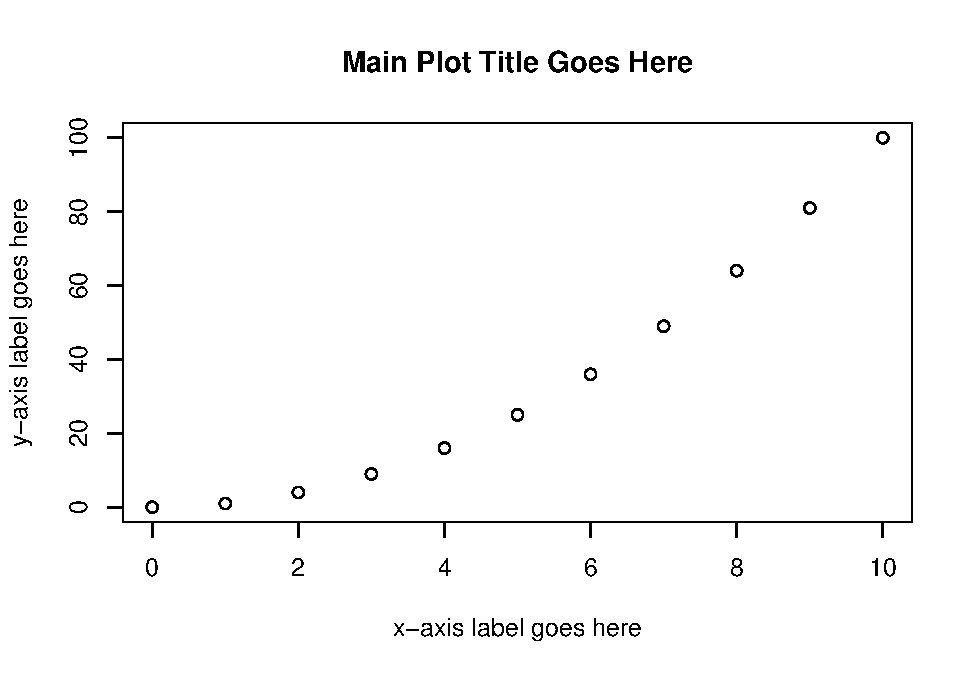
\includegraphics{au-r-workshop_files/figure-latex/unnamed-chunk-70-1} \end{center}

There are a few components:

\begin{itemize}
\tightlist
\item
  The \textbf{plotting region}: all data information is displayed here.
\item
  The \textbf{margin}: where axis labels, tick marks, and main plot
  titles are located
\item
  The \textbf{outer margin}: by default, there is no outer margin. You
  can add one if you want to add text here or make more room around the
  edges.
\end{itemize}

You can change just about everything there is about this plot to suit
your tastes. Duplicate this plot, but make the x-axis, y-axis, and main
titles other than the placeholders shown here:

\begin{Shaded}
\begin{Highlighting}[]
\NormalTok{x =}\StringTok{ }\DecValTok{0}\OperatorTok{:}\DecValTok{10}
\NormalTok{y =}\StringTok{ }\NormalTok{x}\OperatorTok{^}\DecValTok{2}

\KeywordTok{plot}\NormalTok{(}\DataTypeTok{x =}\NormalTok{ x, }\DataTypeTok{y =}\NormalTok{ y,}
     \DataTypeTok{xlab =} \StringTok{"x-axis label goes here"}\NormalTok{, }
     \DataTypeTok{ylab =} \StringTok{"y-axis label goes here"}\NormalTok{,}
     \DataTypeTok{main =} \StringTok{"Main Plot Title Goes Here"}\NormalTok{)}
\end{Highlighting}
\end{Shaded}

Note that the first two arguments, \texttt{x} and \texttt{y}, specify
the coordinates of the points (i.e., the first point is placed at
coordinates \texttt{x{[}1{]}},\texttt{y{[}1{]}}). \texttt{plot} has
\emph{tons} of arguments (or \emph{graphical parameters} as the help
file found using \texttt{?plot} or \texttt{?par} calls them) that change
how the plot looks. Note that when you want something displayed verbatim
on the plotting device, you must wrap that code in \texttt{"\ "}, i.e.,
the arguments \texttt{xlab}, \texttt{ylab}, and \texttt{main} all
receive a character vector of length 1 as input.

Here are just a handful of them to get you started:

\begin{table}

\caption{\label{tab:plot-arg-table}Several of the key arguments to high- and low-level plotting functions}
\centering
\begin{tabular}[t]{l|l|l}
\hline
Arg. & Usage & Description\\
\hline
`xlab` & `xlab = "X-AXIS"` & changes the x-axis label text\\
\hline
`ylab` & `ylab = "Y-AXIS"` & changes the y-axis label text\\
\hline
`main` & `main = "TITLE"` & changes the main title text\\
\hline
`cex` & `cex = 1.5` & changes the size of symbols in the plotting region\textasciicircum{}[`cex` is a multiplier: `cex = 1.5` says make the points 1.5 times as large as they would be by default.]\\
\hline
`pch` & `pch = 17` & changes the symbol type\textasciicircum{}[There are approximately 20 different `pch` settings: `pch = 1` is empty circles, `pch = 16` is filled circles, etc.]\\
\hline
`xlim` & `xlim = range(x)` & changes the endpoints (limits) of the x-axis\textasciicircum{}[`xlim` and `ylim` both require a numeric vector of length 2 where neither of the elements may be an `NA`.]\\
\hline
`ylim` & `ylim = c(0,1)` & same as `xlim`, but for the y-axis\\
\hline
`type` & `type = "l"` & changes the way points are connected by lines\textasciicircum{}[The default is points only, `type = "l"` is for lines only, `type = "o"` is for points connected with lines, and `type = "b"` is for points and lines but with a small amount of separation between them.]\\
\hline
`lty` & `lty = 2` & changes the line type\textasciicircum{}[`lty = 1` is solid, `lty = 2` is dashed, `lty = 3` is dotted, etc. You can also specific it like `lty = "solid"`, `lty = "dotted"`, or `lty = "dotdash"`.]\\
\hline
`lwd` & `lwd = 2` & changes the line width\textasciicircum{}[works just like `cex`: `lwd = 3` codes for a line that is 3 times as thick as it would normally be]\\
\hline
`col` & `col = "blue"` & changes the color of plotted objects\textasciicircum{}[there is a whole host of colors you can pass R by name, run `colors()` to see for yourself]\\
\hline
\end{tabular}
\end{table}

You are advised to try at least some of these arguments out for yourself
with your \texttt{plot(x,\ y)} code from above - notice how every time
you run \texttt{plot}, a whole new plot is created, not just the thing
you changed. There are definitely other options: check out
\texttt{?plot} or \texttt{?par} for more details.

\section{Lower Level Plotting
Functions}\label{lower-level-plotting-functions}

Now that you have a base plot designed to your liking, you might want to
add some additional ``layers'' to it to represent more data or other
kind of information like an additional label or text. Add some more
points to your plot by putting this line right beneath your
\texttt{plot(x,y)} code and run just the \texttt{points()} line (make
sure your device is showing a plot first):

\begin{Shaded}
\begin{Highlighting}[]
\CommentTok{# rev() reverses a vector: so the old x[1] is x[11] now}
\KeywordTok{points}\NormalTok{(}\DataTypeTok{x =} \KeywordTok{rev}\NormalTok{(x), }\DataTypeTok{y =}\NormalTok{ y, }\DataTypeTok{col =} \StringTok{"blue"}\NormalTok{, }\DataTypeTok{pch =} \DecValTok{16}\NormalTok{)}
\end{Highlighting}
\end{Shaded}

\begin{center}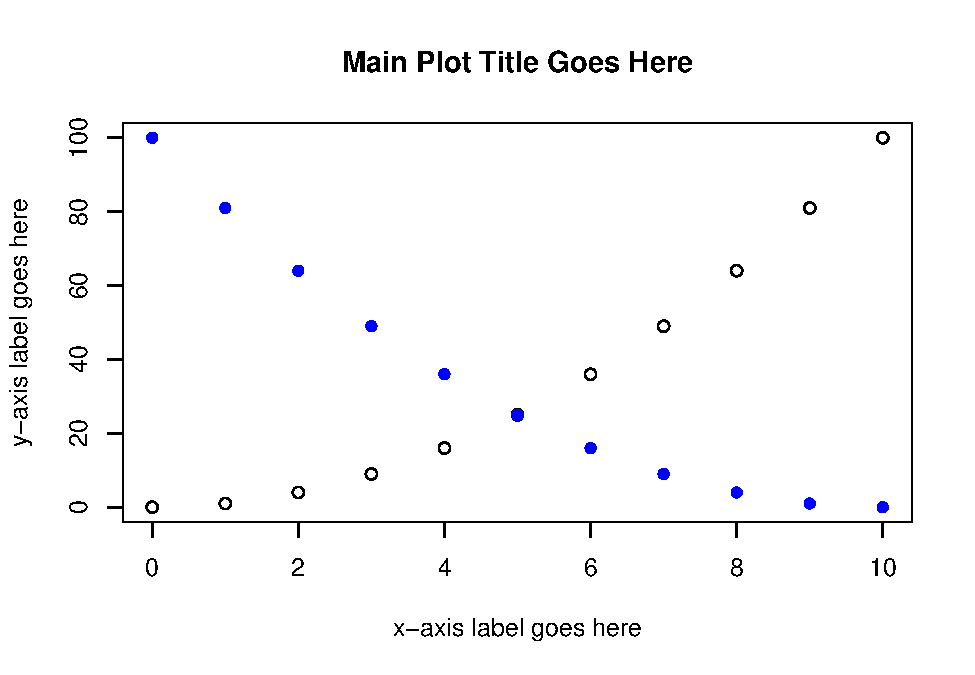
\includegraphics{au-r-workshop_files/figure-latex/unnamed-chunk-73-1} \end{center}

Here, \texttt{points} acted like a low-level plotting function because
it added points to a plot you already made. Many of the arguments shown
in Table \ref{tab:plot-arg-table} can be used in both high-level and
low-level plotting functions (notice how \texttt{col} and \texttt{pch}
were used in \texttt{points}). Just like \texttt{points}, there is also
\texttt{lines}:

\begin{Shaded}
\begin{Highlighting}[]
\KeywordTok{lines}\NormalTok{(}\DataTypeTok{x =}\NormalTok{ x, }\DataTypeTok{y =}\NormalTok{ x, }\DataTypeTok{lty =} \DecValTok{2}\NormalTok{, }\DataTypeTok{col =} \StringTok{"red"}\NormalTok{)}
\end{Highlighting}
\end{Shaded}

\begin{center}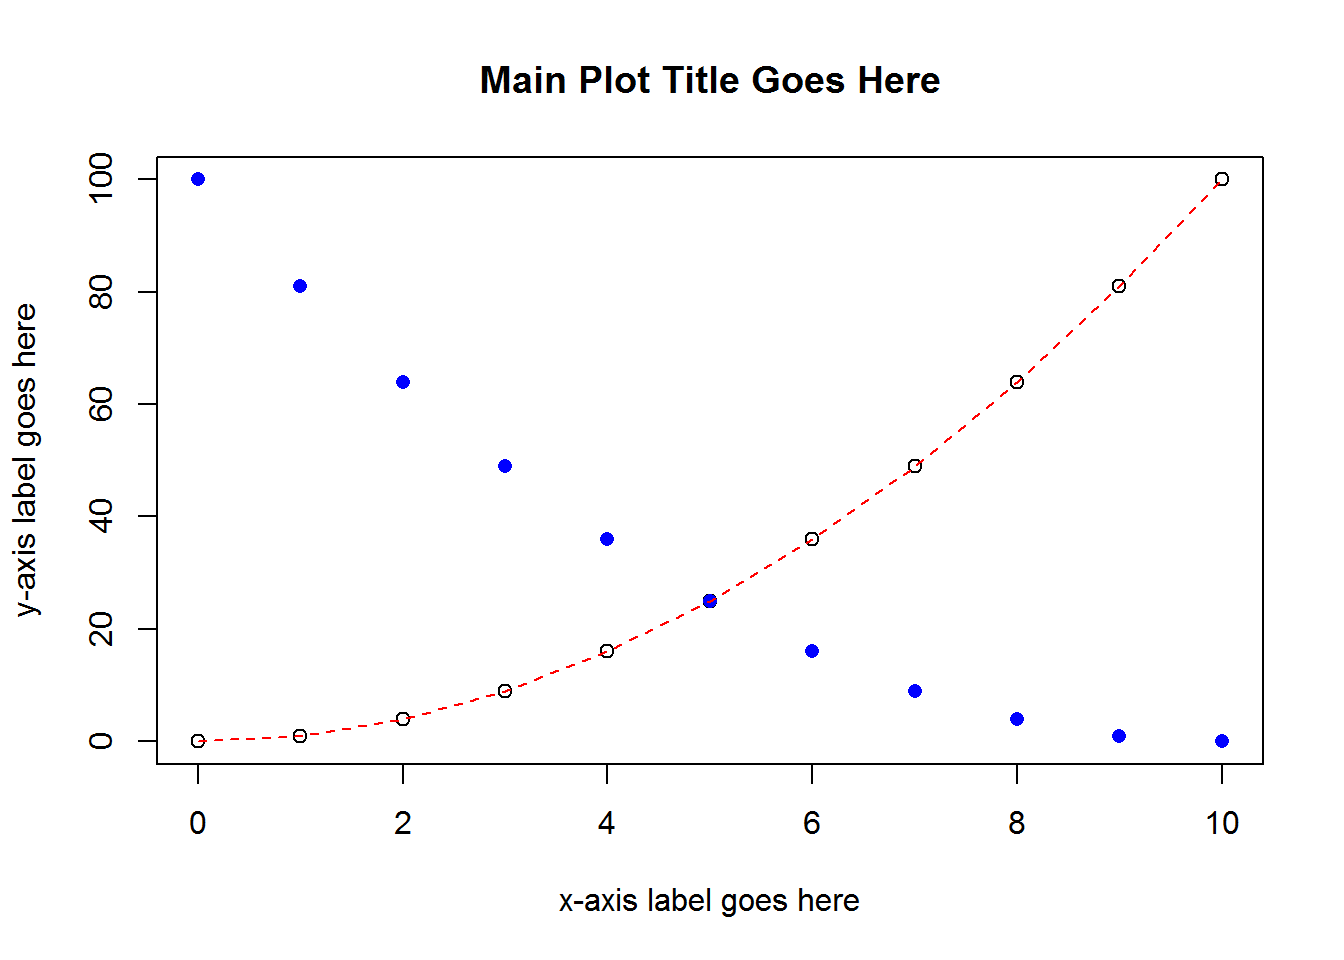
\includegraphics{au-r-workshop_files/figure-latex/unnamed-chunk-75-1} \end{center}

You can also add text to the plotting region:

\begin{Shaded}
\begin{Highlighting}[]
\KeywordTok{text}\NormalTok{(}\DataTypeTok{x =} \DecValTok{5}\NormalTok{, }\DataTypeTok{y =} \DecValTok{80}\NormalTok{, }\StringTok{"This is Text"}\NormalTok{, }\DataTypeTok{cex =} \FloatTok{1.5}\NormalTok{, }\DataTypeTok{col =} \StringTok{"grey"}\NormalTok{, }\DataTypeTok{font =} \DecValTok{4}\NormalTok{)}
\end{Highlighting}
\end{Shaded}

\begin{center}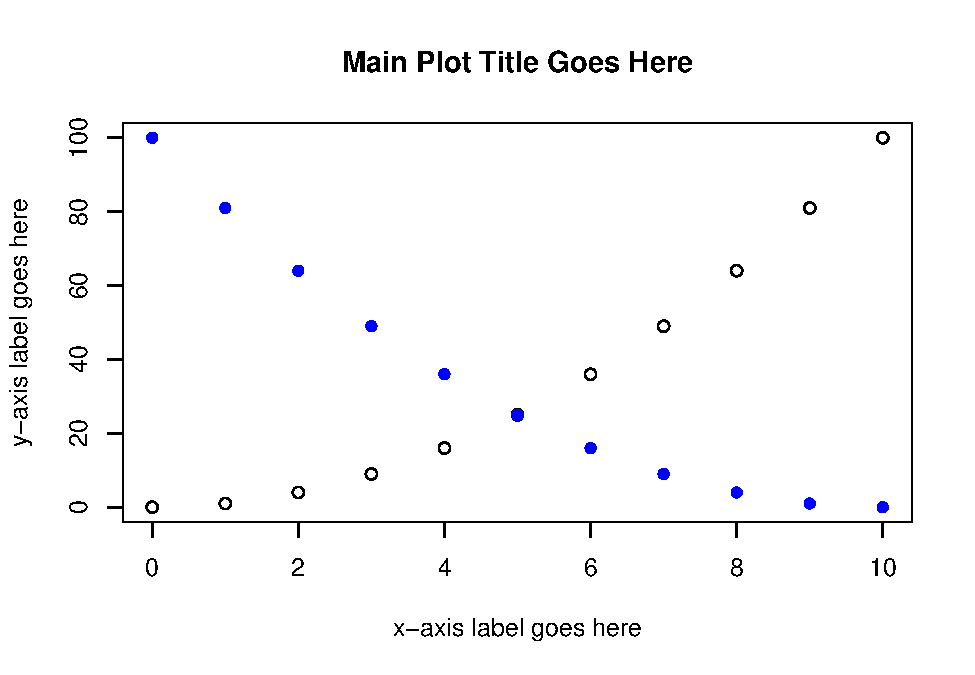
\includegraphics{au-r-workshop_files/figure-latex/unnamed-chunk-77-1} \end{center}

The text is centered on the coordinates you provide. You can also
provide vectors of coordinates and text to write different things at
once.

The easiest way to add a straight line to a plot is with
\texttt{abline}. By default it takes two arguments: \texttt{a} and
\texttt{b} which are the intercept and slope, respectively, e.g.,
\texttt{abline(c(0,1))} will draw a 1:1 line. You can also do
\texttt{abline(h\ =\ 5)} to draw a horizontal line at 5 or
\texttt{abline(v\ =\ 5)} to draw a vertical line at \texttt{5}.

You can see that the text is centered on the coordinates
\texttt{x\ =\ 5} and \texttt{y\ =\ 80} using \texttt{abline}:

\begin{Shaded}
\begin{Highlighting}[]
\KeywordTok{abline}\NormalTok{(}\DataTypeTok{h =} \DecValTok{80}\NormalTok{, }\DataTypeTok{col =} \StringTok{"grey"}\NormalTok{)}
\KeywordTok{abline}\NormalTok{(}\DataTypeTok{v =} \DecValTok{5}\NormalTok{, }\DataTypeTok{col =} \StringTok{"grey"}\NormalTok{)}
\end{Highlighting}
\end{Shaded}

\begin{center}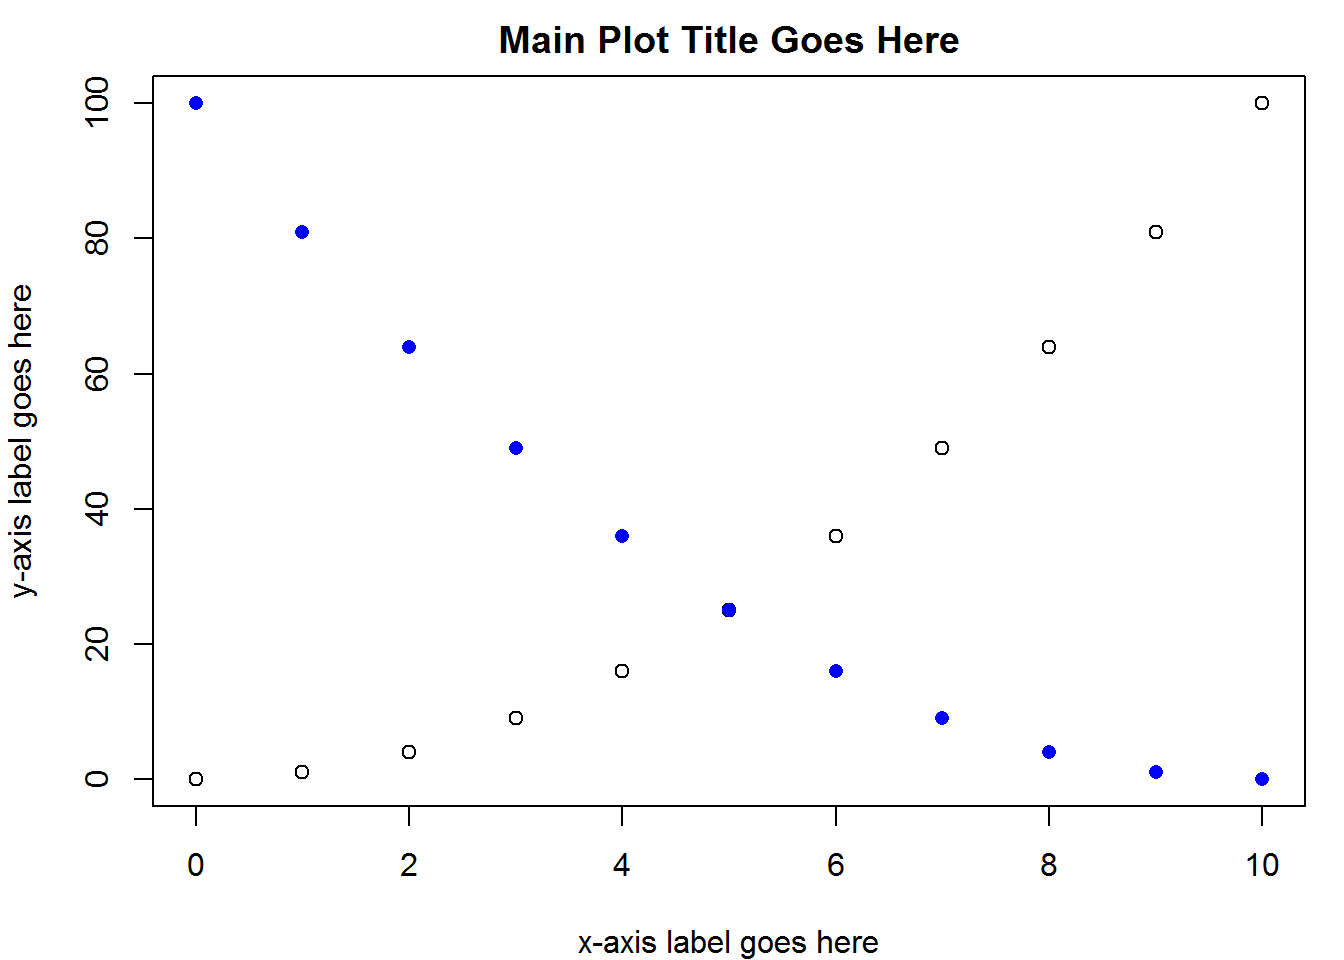
\includegraphics{au-r-workshop_files/figure-latex/unnamed-chunk-79-1} \end{center}

If you accidentally add a plot element that you don't want using a
low-level plotting function, the only way to remove it is by re-running
the high-level plotting function to start a new plot and adding only the
objects you want. Try removing the ``This is Text'' text and the
straight lines you drew with \texttt{abline} from the plot displayed in
your device.

\section{Other High-Level Plotting
Functions}\label{other-high-level-plotting-functions}

You have just seen the basics of making two dimensional scatter plots
and line plots. You will now explore other types of graphs you can make.

\subsection{The Bar Graph}\label{the-bar-graph}

Another very common graph is a bar graph. R has a \texttt{bargraph}
function, and again, it has lots of arguments. Here you will just make
two common variations: single bars per group and multiple bars per
group. Let's make up some data to plot:

\begin{Shaded}
\begin{Highlighting}[]
\NormalTok{x1 =}\StringTok{ }\KeywordTok{c}\NormalTok{(}\DecValTok{2}\NormalTok{,}\DecValTok{4}\NormalTok{,}\DecValTok{6}\NormalTok{)}
\KeywordTok{barplot}\NormalTok{(x1)}
\end{Highlighting}
\end{Shaded}

\begin{center}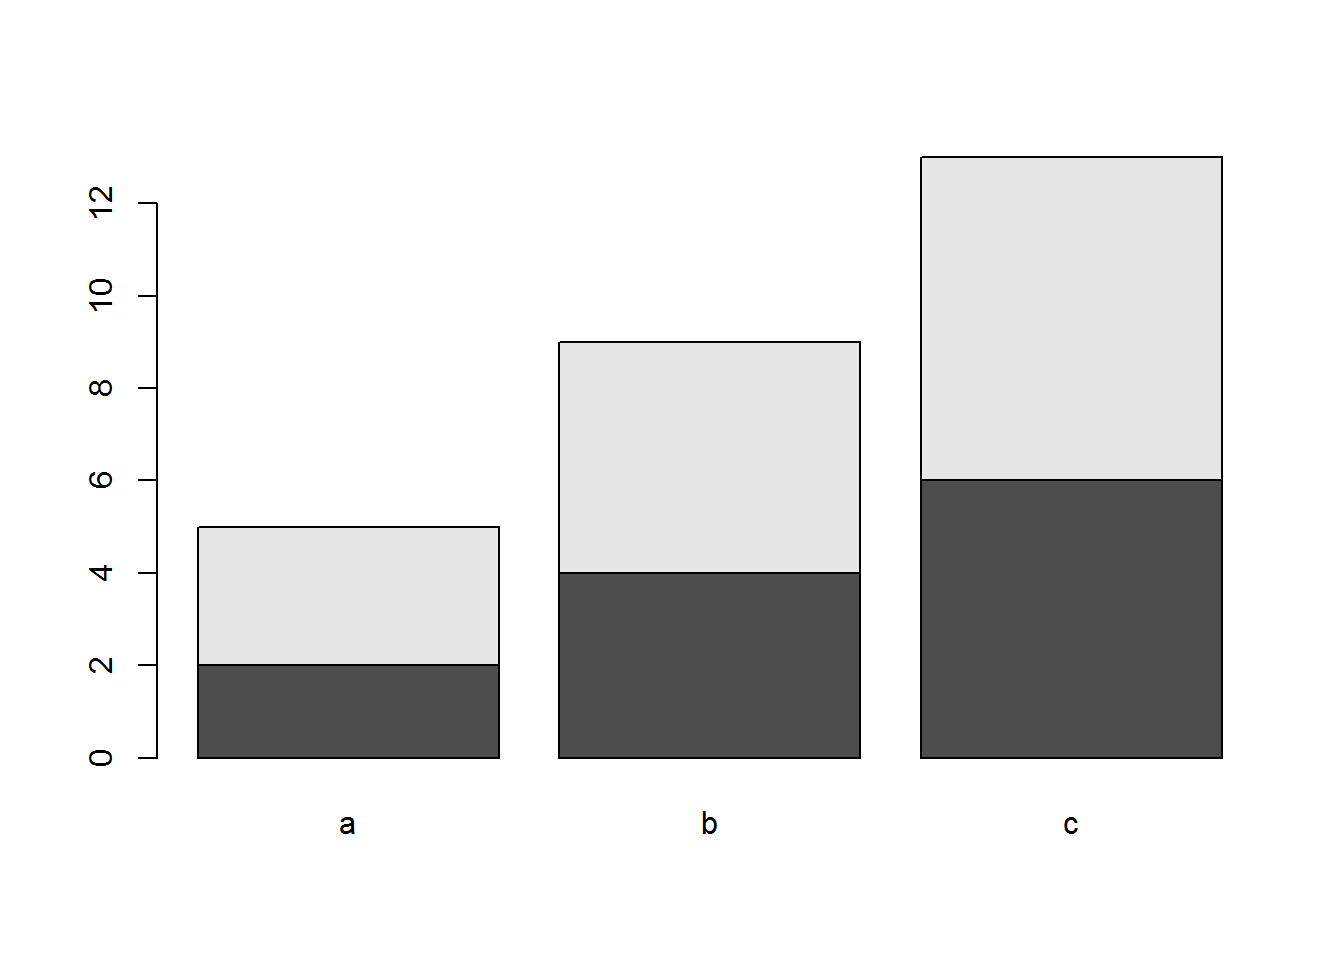
\includegraphics{au-r-workshop_files/figure-latex/unnamed-chunk-80-1} \end{center}

Notice that there are no group names on our bars (if our vector had
names, there would be). You can add names by using the argument
\texttt{names.arg}:

\begin{Shaded}
\begin{Highlighting}[]
\KeywordTok{barplot}\NormalTok{(x1, }\DataTypeTok{names.arg =} \KeywordTok{c}\NormalTok{(}\StringTok{"a"}\NormalTok{, }\StringTok{"b"}\NormalTok{, }\StringTok{"c"}\NormalTok{))}
\end{Highlighting}
\end{Shaded}

Add some more information by including two bars per group. Make some
more data and combine it with the old data:

\begin{Shaded}
\begin{Highlighting}[]
\NormalTok{x2 =}\StringTok{ }\KeywordTok{c}\NormalTok{(}\DecValTok{3}\NormalTok{,}\DecValTok{5}\NormalTok{,}\DecValTok{7}\NormalTok{)}
\NormalTok{x3 =}\StringTok{ }\KeywordTok{rbind}\NormalTok{(x1, x2)}

\KeywordTok{barplot}\NormalTok{(x3, }\DataTypeTok{names.arg =} \KeywordTok{c}\NormalTok{(}\StringTok{"a"}\NormalTok{, }\StringTok{"b"}\NormalTok{, }\StringTok{"c"}\NormalTok{), }\DataTypeTok{beside =}\NormalTok{ T)}
\end{Highlighting}
\end{Shaded}

\begin{center}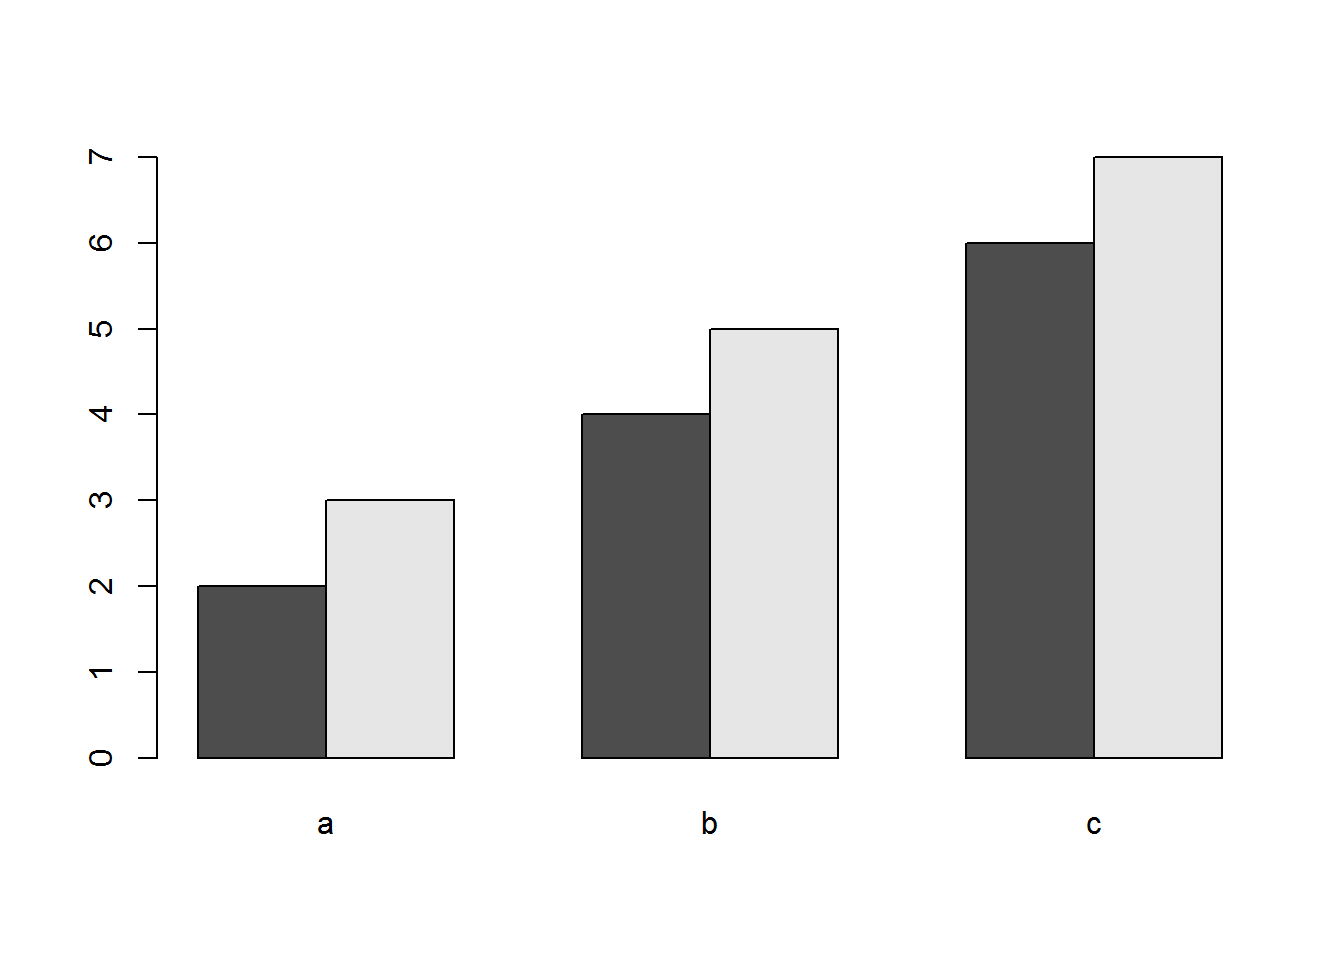
\includegraphics{au-r-workshop_files/figure-latex/unnamed-chunk-82-1} \end{center}

To add multiple bars per group, R needs a matrix like you just made. The
\textbf{columns} store the heights of the bars that will be placed
together in a group. Including the \texttt{beside\ =\ T} argument tells
R to plot all groups as different bars as opposed to using a stacked bar
graph.

Oftentimes, we want to add error bars to a bar graph like this. To avoid
digressing too much here, creating error bars is covered as a bonus
topic.

\section{Box-and-Whisker Plots}\label{box-whisker}

Box-and-whisker plots are a great way to visualize the spread of your
data. All you need to make a box-and-whisker plot is a grouping variable
(a factor, revisit Section \ref{factors} if you don't remember what
these are) and some continuous (i.e., numeric) data for each level of
the factor. Download the \texttt{creel.csv} data set from the GitHub
repository
\url{https://github.com/bstaton1/au-r-workshop-data/tree/master}, place
it in the same directory as your R script \texttt{Ch2.R} (which is the
one you should be working on right now).

Read the data in and print a summary:

\begin{Shaded}
\begin{Highlighting}[]
\NormalTok{dat =}\StringTok{ }\KeywordTok{read.csv}\NormalTok{(}\StringTok{"creel.csv"}\NormalTok{)}
\KeywordTok{summary}\NormalTok{(dat)}
\end{Highlighting}
\end{Shaded}

\begin{verbatim}
##            fishery        hours       
##  Harvest       :100   Min.   :-1.150  
##  Non.Tournament:100   1st Qu.: 9.936  
##  Tournament    :100   Median :20.758  
##                       Mean   :26.050  
##                       3rd Qu.:43.896  
##                       Max.   :62.649
\end{verbatim}

This data set contains some simulated (i.e., fake) continuous and
categorical data that represent 300 anglers who were creel
surveyed\footnote{A creel survey is a sampling program where fishers are
  asked questions about their fishing behavior in order to estimate
  effort and harvest.}. In the data set, there are three categories
(levels to the factor \texttt{fishery}) and the continuous variable is
how many hours each angler fished this year. If you supply the generic
\texttt{plot} function with a continuous response (\texttt{y}) variable
and a categorical predictor (\texttt{x}) variable, it will automatically
know that you want to make a box-and-whisker plot:

\begin{Shaded}
\begin{Highlighting}[]
\KeywordTok{plot}\NormalTok{(}\DataTypeTok{x =}\NormalTok{ dat}\OperatorTok{$}\NormalTok{fishery, }\DataTypeTok{y =}\NormalTok{ dat}\OperatorTok{$}\NormalTok{hours)}
\end{Highlighting}
\end{Shaded}

\begin{center}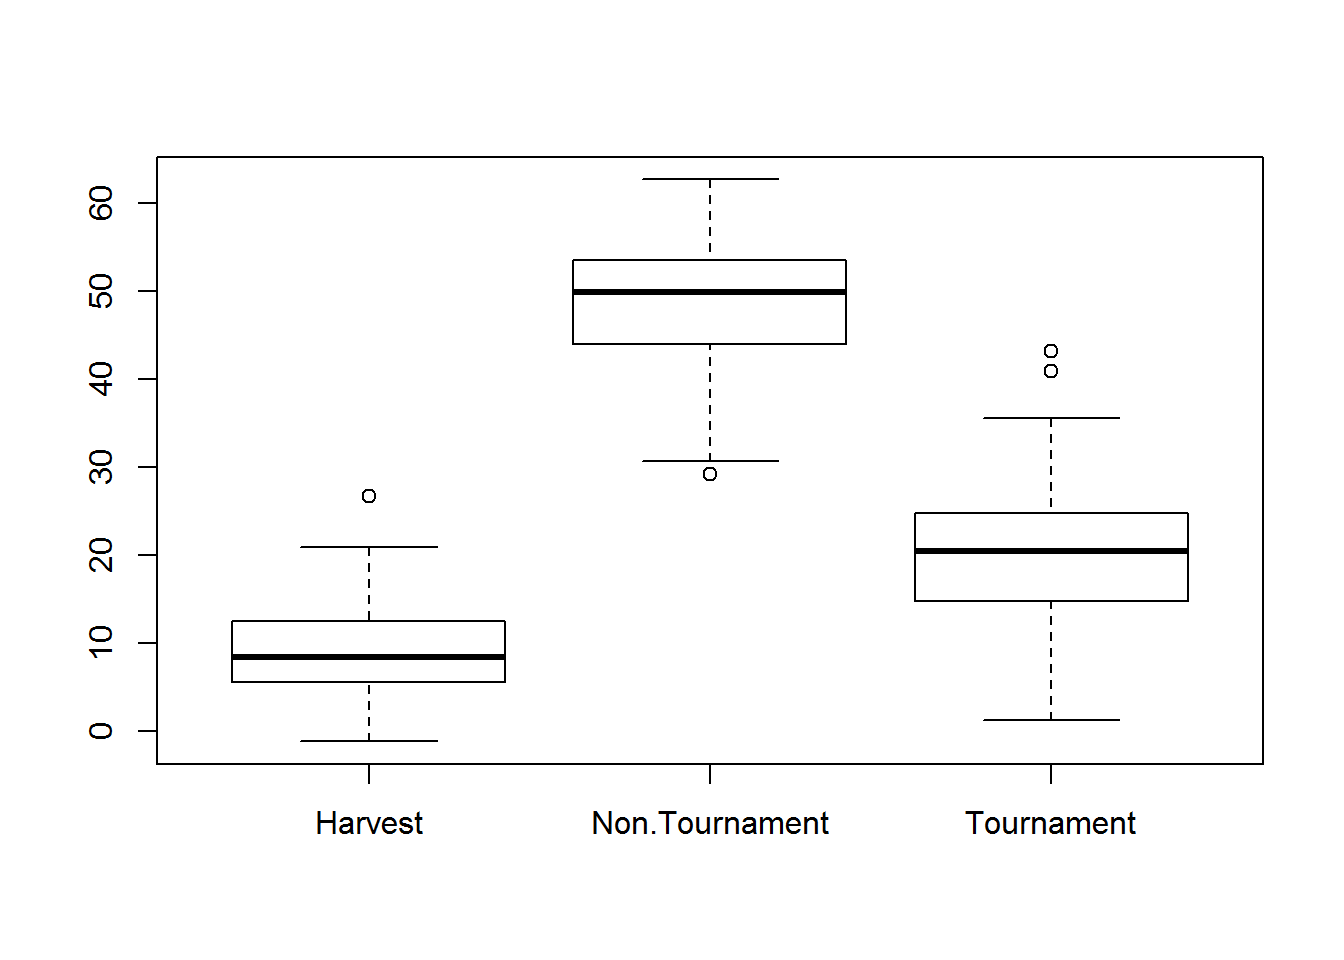
\includegraphics{au-r-workshop_files/figure-latex/unnamed-chunk-85-1} \end{center}

In the box-and-whisker plot above, the heavy line is the median, the
ends of the boxes are the 25\textsuperscript{th} and
75\textsuperscript{th} percentiles and the ``whiskers'' are the
2.5\textsuperscript{th} and 97.5\textsuperscript{th} percentiles. Any
points that are outliers (i.e., fall outside of the whiskers) will be
shown as points\footnote{Outliers can be turned off using the
  \texttt{outline\ =\ F} argument to the \texttt{plot} function}.

It is worth introducing a shorthand syntax of typing the same command:

\begin{Shaded}
\begin{Highlighting}[]
\KeywordTok{plot}\NormalTok{(hours }\OperatorTok{~}\StringTok{ }\NormalTok{fishery, }\DataTypeTok{data =}\NormalTok{ dat)}
\end{Highlighting}
\end{Shaded}

Instead of saying \texttt{plot(x\ =\ x.var,\ y\ =\ y.var)}, this
expression says \texttt{plot(y.var\ \textasciitilde{}\ x.var)}. The
\texttt{\textasciitilde{}} reads ``as a function of''. By specifying the
\texttt{data} argument, you no longer need to indicate where the
variables \texttt{hours} and \texttt{fishery} are found. Many R
functions have a \texttt{data} argument that works this same way. It is
sometimes preferable to plot variables with this syntax because it is
often less code and is also the format of R's statistical
equations\footnote{Which allows you to easily copy and paste the code
  between the model and plot functions, see Chapter \ref{ch3}}.

\section{Histograms}\label{histograms}

Another way to show the distribution of a variable is with histograms.
These figures show the relative frequencies of observations in different
discrete bins. Let's make a histogram of hours the surveyed tournament
anglers fished this year:

\begin{Shaded}
\begin{Highlighting}[]
\KeywordTok{hist}\NormalTok{(dat}\OperatorTok{$}\NormalTok{hours[dat}\OperatorTok{$}\NormalTok{fishery }\OperatorTok{==}\StringTok{ "Tournament"}\NormalTok{])}
\end{Highlighting}
\end{Shaded}

\begin{center}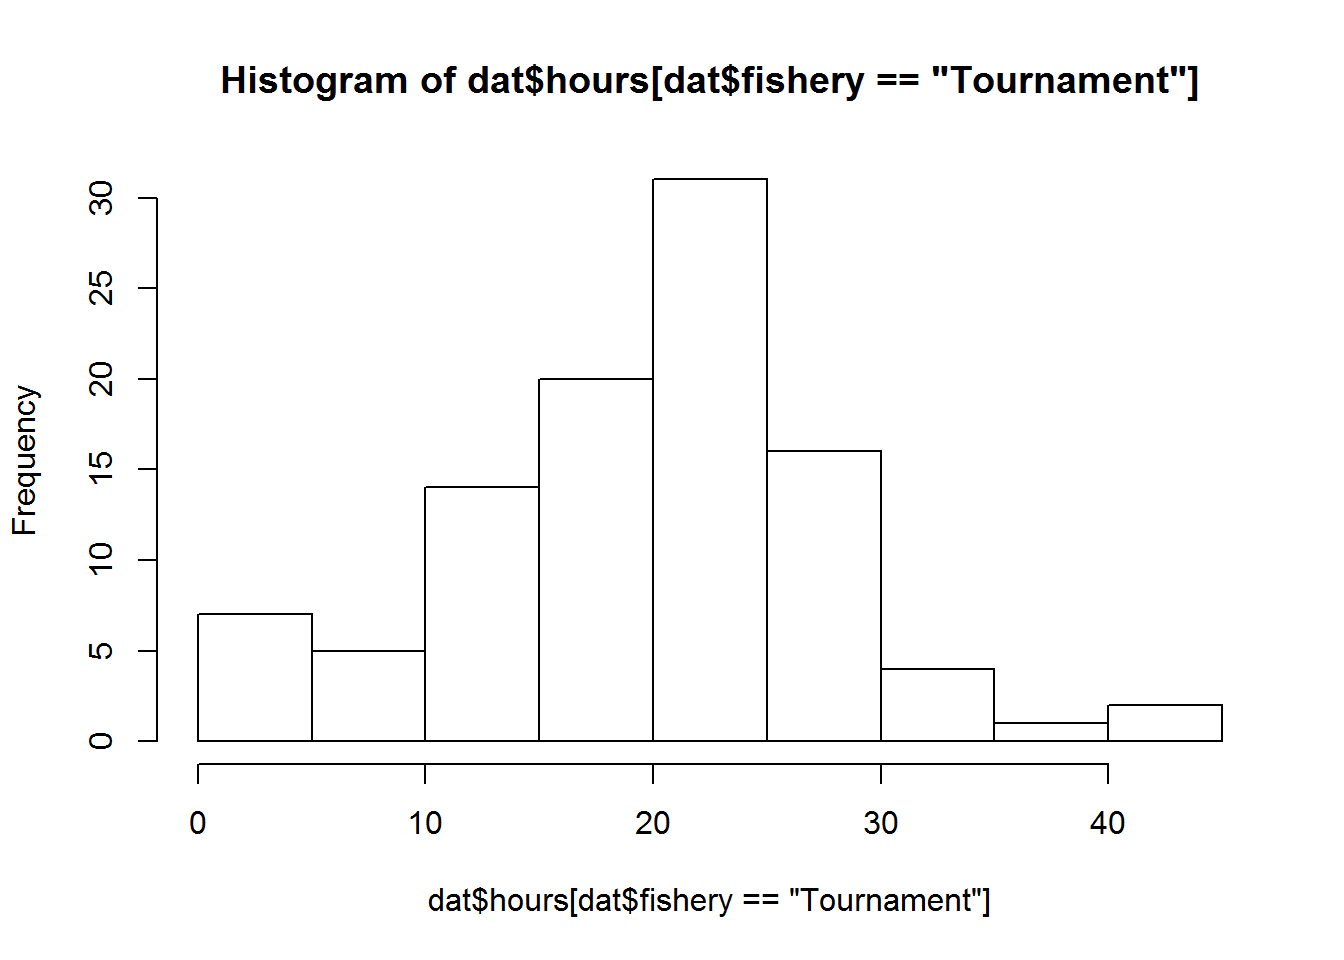
\includegraphics{au-r-workshop_files/figure-latex/unnamed-chunk-87-1} \end{center}

Notice the subset that extracts hours fished for tournament anglers only
before plotting.

\texttt{hist} automatically selects the number of bins based on the
range and resolution of the data. You can specify how many evenly-sized
bins you want to plot:

\begin{Shaded}
\begin{Highlighting}[]
\CommentTok{# extract the hours for tournament anglers}
\NormalTok{t_hrs =}\StringTok{ }\NormalTok{dat}\OperatorTok{$}\NormalTok{hours[dat}\OperatorTok{$}\NormalTok{fishery }\OperatorTok{==}\StringTok{ "Tournament"}\NormalTok{]}

\CommentTok{# create the bin endpoints}
\NormalTok{nbins =}\StringTok{ }\DecValTok{20}
\NormalTok{breaks =}\StringTok{ }\KeywordTok{seq}\NormalTok{(}\DataTypeTok{from =} \KeywordTok{min}\NormalTok{(t_hrs), }\DataTypeTok{to =} \KeywordTok{max}\NormalTok{(t_hrs), }\DataTypeTok{length =}\NormalTok{ nbins }\OperatorTok{+}\StringTok{ }\DecValTok{1}\NormalTok{)}
\KeywordTok{hist}\NormalTok{(t_hrs, }\DataTypeTok{breaks =}\NormalTok{ breaks, }\DataTypeTok{main =} \StringTok{"Tournament"}\NormalTok{, }\DataTypeTok{col =} \StringTok{"grey"}\NormalTok{)}
\end{Highlighting}
\end{Shaded}

\begin{center}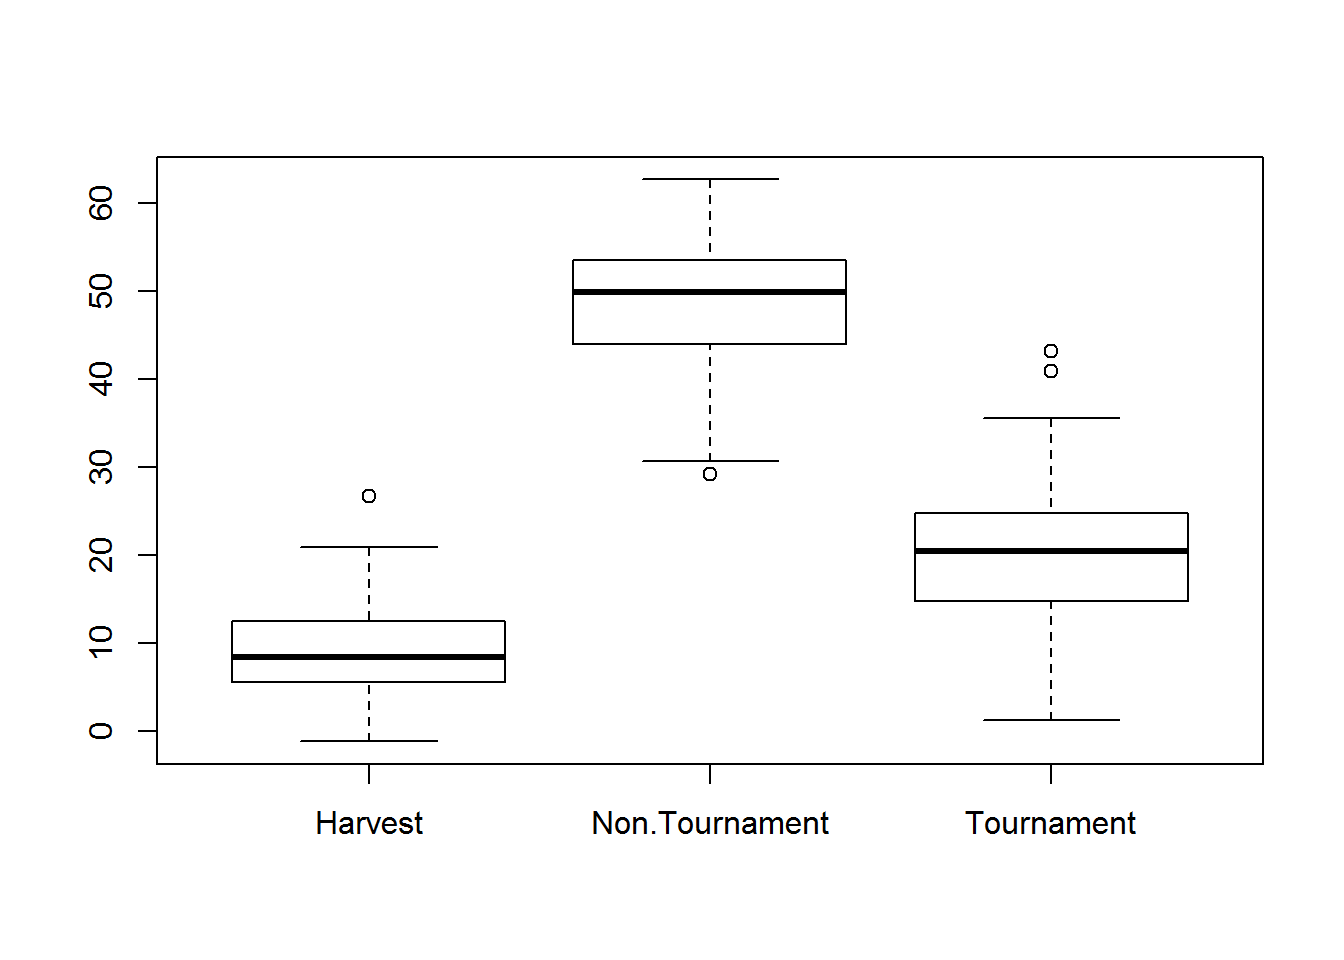
\includegraphics{au-r-workshop_files/figure-latex/unnamed-chunk-88-1} \end{center}

\section{\texorpdfstring{The \texttt{par}
Function}{The par Function}}\label{the-par-function}

If it bothers you that the axes are ``floating'', you can fix this using
this command:

\begin{Shaded}
\begin{Highlighting}[]
\KeywordTok{par}\NormalTok{(}\DataTypeTok{xaxs =} \StringTok{"i"}\NormalTok{, }\DataTypeTok{yaxs =} \StringTok{"i"}\NormalTok{)}
\KeywordTok{hist}\NormalTok{(t_hrs, }\DataTypeTok{breaks =}\NormalTok{ breaks, }\DataTypeTok{main =} \StringTok{"Tournament"}\NormalTok{, }\DataTypeTok{col =} \StringTok{"grey"}\NormalTok{)}
\end{Highlighting}
\end{Shaded}

\begin{center}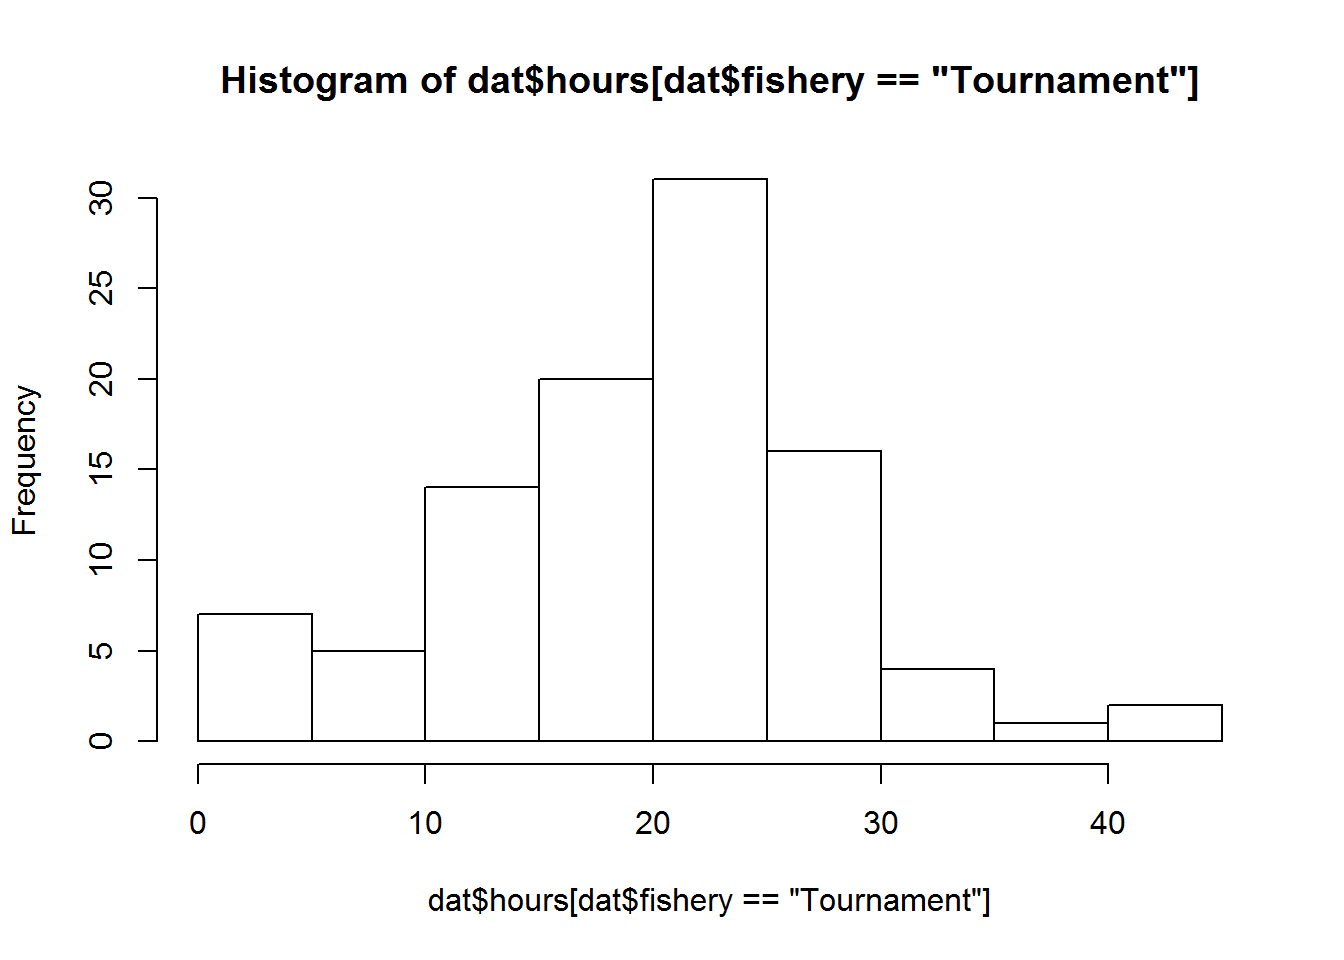
\includegraphics{au-r-workshop_files/figure-latex/unnamed-chunk-89-1} \end{center}

Here, you changed the graphical parameters of the graphics device by
using the \texttt{par} argument. Once you change the settings in
\texttt{par}, they will remain that way until you start a new device.

The \texttt{par} function is central to fine-tuning your graphics. Here,
the \texttt{xaxs\ =\ "i"} and \texttt{yaxs\ =\ "i"} arguments
essentially removed the buffer between the data and the axes.
\texttt{par} has options to change the size of the margins, add outer
margins, change colors, etc. Some of the graphical parameters that can
be passed to high- and low-level plotting functions (like those in Table
\ref{tab:plot-arg-table}) can also be passed \texttt{par}. Check out the
help file (\texttt{?par}) to see everything it can do. If you want to
start over with fresh \texttt{par} settings, start a new device.

\section{New Temporary Devices}\label{new-temporary-devices}

If you are using RStudio, then likely all of the plots you have made
thus far have shown up in the lower right-hand corner or your RStudio
window. You have been using RStudio's built-in plotting device. If you
wish to open a new plotting device (maybe to put it on a separate
monitor), you can use the following commands, depending on your
operating system:

\begin{itemize}
\tightlist
\item
  \textbf{Windows Users} -- just run \texttt{windows()} to open up a new
  plotting device. It will become the active device.
\item
  \textbf{Mac Users} -- similarly, you can run \texttt{quartz()} to open
  a new device.
\item
  \textbf{Linux Users} -- similarly, just run \texttt{x11()}.
\end{itemize}

\section{Multi-panel Plots}\label{multi-panel-plots}

Sometimes you want to display more than one plot at a time. You can make
a multi-panel plot which allows for multiple plotting regions to show up
simultaneously within the same plotting device. First, you need to
change the layout of the plotting region. The easiest way to set up the
device for multi-panel plotting is by using the \texttt{mfrow} argument
in the \texttt{par} function.

Below, the code says ``set up change the graphical parameters so that
there is 1 row and 3 columns of plotting regions within the device''.
Every time you make a new plot, it will go in the next available
plotting region. Make 3 histograms, each that represents a different
sector of the fishery:

\begin{Shaded}
\begin{Highlighting}[]
\KeywordTok{par}\NormalTok{(}\DataTypeTok{mfrow =} \KeywordTok{c}\NormalTok{(}\DecValTok{1}\NormalTok{,}\DecValTok{3}\NormalTok{))}
\KeywordTok{hist}\NormalTok{(dat}\OperatorTok{$}\NormalTok{hours[dat}\OperatorTok{$}\NormalTok{fishery }\OperatorTok{==}\StringTok{ "Tournament"}\NormalTok{], }\DataTypeTok{main =} \StringTok{"Tourn"}\NormalTok{)}
\KeywordTok{hist}\NormalTok{(dat}\OperatorTok{$}\NormalTok{hours[dat}\OperatorTok{$}\NormalTok{fishery }\OperatorTok{==}\StringTok{ "Non.Tournament"}\NormalTok{], }\DataTypeTok{main =} \StringTok{"Non.Tourn"}\NormalTok{)}
\KeywordTok{hist}\NormalTok{(dat}\OperatorTok{$}\NormalTok{hours[dat}\OperatorTok{$}\NormalTok{fishery }\OperatorTok{==}\StringTok{ "Harvest"}\NormalTok{], }\DataTypeTok{main =} \StringTok{"Harvest"}\NormalTok{)}
\end{Highlighting}
\end{Shaded}

\begin{center}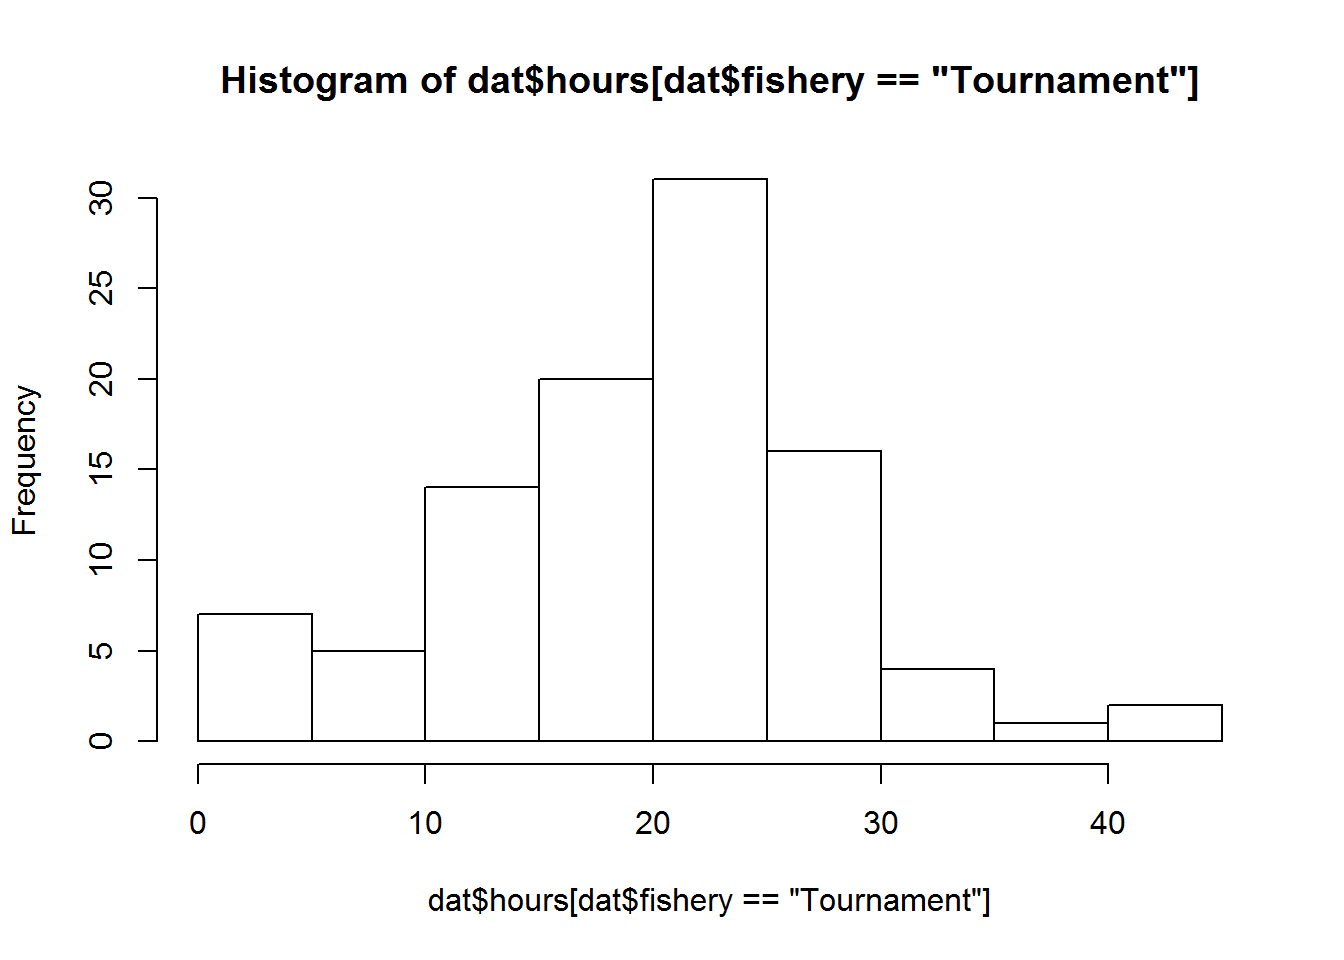
\includegraphics{au-r-workshop_files/figure-latex/unnamed-chunk-90-1} \end{center}

There are other ways to make multi-panel plots, however, they are beyond
the scope of this beginner's workshop. See \texttt{?layout} for details.
With this function you can change the size of certain plots and make
them have different shapes (i.e., some squares, some rectangles, etc.),
but it takes some pretty involved (though not impossible, by any means)
specification of how you want the device to be split up into regions.

\section{Legends}\label{legends}

Oftentimes you will want to add a legend to our plots to help people
interpret what it is showing. You can add legends to R plots using the
low-level plotting function \texttt{legend}. Add a legend to the bar
plot you made earlier with two groups. First, re-make the plot by
running the high-level \texttt{barplot} function, but change the colors
of the bars to be shades of blue and red. Once you have the plot made,
add the legend:

\begin{Shaded}
\begin{Highlighting}[]
\KeywordTok{barplot}\NormalTok{(x3, }\DataTypeTok{beside =}\NormalTok{ T,}\DataTypeTok{names.arg =} \KeywordTok{c}\NormalTok{(}\StringTok{"a"}\NormalTok{, }\StringTok{"b"}\NormalTok{, }\StringTok{"c"}\NormalTok{), }\DataTypeTok{col =} \KeywordTok{c}\NormalTok{(}\StringTok{"skyblue2"}\NormalTok{, }\StringTok{"tomato2"}\NormalTok{))}
\KeywordTok{legend}\NormalTok{(}\StringTok{"topleft"}\NormalTok{, }\DataTypeTok{legend =} \KeywordTok{c}\NormalTok{(}\StringTok{"Group 1"}\NormalTok{, }\StringTok{"Group 2"}\NormalTok{), }\DataTypeTok{fill =} \KeywordTok{c}\NormalTok{(}\StringTok{"skyblue2"}\NormalTok{, }\StringTok{"tomato2"}\NormalTok{))}
\end{Highlighting}
\end{Shaded}

\begin{center}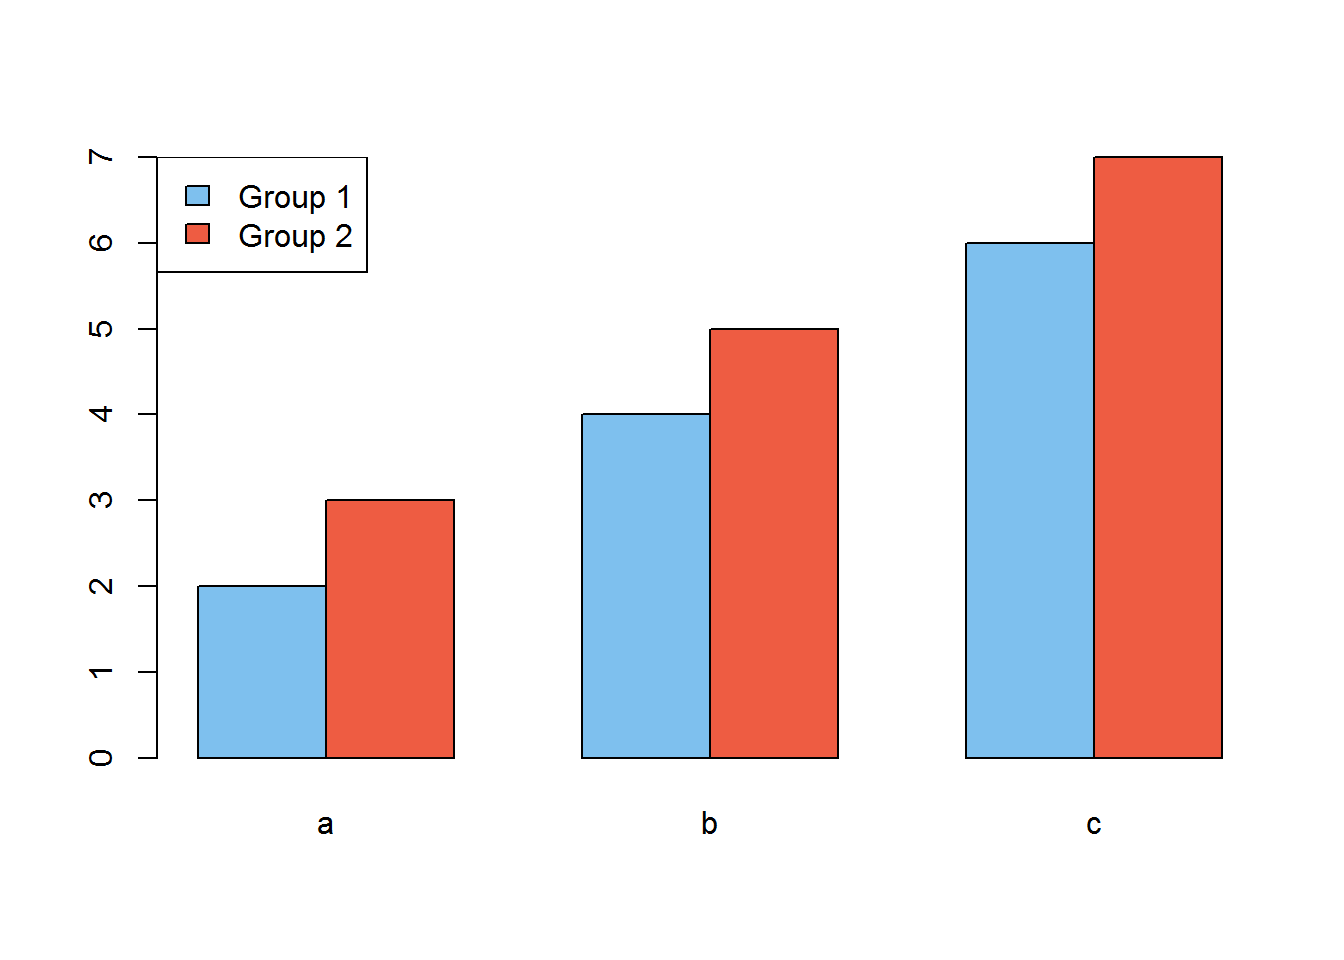
\includegraphics{au-r-workshop_files/figure-latex/unnamed-chunk-91-1} \end{center}

The box can be removed using the \texttt{bty\ =\ "n"} argument and the
size can be changed using \texttt{cex}. The position can be specified
either with words (like above) or by using x-y coordinates.

Here is a more complex example:

\begin{Shaded}
\begin{Highlighting}[]
\CommentTok{# 1) extract and sort the hours for two fisheries from fewest hours}
\NormalTok{t_hrs =}\StringTok{ }\KeywordTok{sort}\NormalTok{(dat}\OperatorTok{$}\NormalTok{hours[dat}\OperatorTok{$}\NormalTok{fishery }\OperatorTok{==}\StringTok{ "Tournament"}\NormalTok{])}
\NormalTok{n_hrs =}\StringTok{ }\KeywordTok{sort}\NormalTok{(dat}\OperatorTok{$}\NormalTok{hours[dat}\OperatorTok{$}\NormalTok{fishery }\OperatorTok{==}\StringTok{ "Non.Tournament"}\NormalTok{])}

\CommentTok{# 2) make the plot: plot for t_hrs only, but ensure xlim covers both groups}
\KeywordTok{par}\NormalTok{(}\DataTypeTok{mar =} \KeywordTok{c}\NormalTok{(}\DecValTok{4}\NormalTok{,}\DecValTok{4}\NormalTok{,}\DecValTok{1}\NormalTok{,}\DecValTok{1}\NormalTok{))  }\CommentTok{# set the margins: 4 lines of margin space on bottom and left, 1 on top and right}
\KeywordTok{plot}\NormalTok{(}\DataTypeTok{x =}\NormalTok{ t_hrs, }\DataTypeTok{y =} \DecValTok{1}\OperatorTok{:}\KeywordTok{length}\NormalTok{(t_hrs),}
     \DataTypeTok{type =} \StringTok{"o"}\NormalTok{, }\DataTypeTok{lty =} \DecValTok{2}\NormalTok{, }\DataTypeTok{xlim =} \KeywordTok{range}\NormalTok{(}\KeywordTok{c}\NormalTok{(t_hrs, n_hrs)),}
     \DataTypeTok{xlab =} \StringTok{"Hours Fished/Year"}\NormalTok{, }\DataTypeTok{ylab =} \StringTok{"Rank within Fishery Samples"}\NormalTok{,}
     \DataTypeTok{las =} \DecValTok{1}\NormalTok{)  }\CommentTok{# las = 1 says "turn the y-axis tick labels to be horizontal"}

\CommentTok{# 3) add info for the other fishery}
\KeywordTok{points}\NormalTok{(}\DataTypeTok{x =}\NormalTok{ n_hrs, }\DataTypeTok{y =} \DecValTok{1}\OperatorTok{:}\KeywordTok{length}\NormalTok{(n_hrs), }\DataTypeTok{type =} \StringTok{"o"}\NormalTok{, }\DataTypeTok{lty =} \DecValTok{1}\NormalTok{, }\DataTypeTok{pch =} \DecValTok{16}\NormalTok{)}

\CommentTok{# 4) add the legend}
\KeywordTok{legend}\NormalTok{(}\StringTok{"topleft"}\NormalTok{, }\DataTypeTok{legend =} \KeywordTok{c}\NormalTok{(}\StringTok{"Tournament"}\NormalTok{, }\StringTok{"Non-Tournament"}\NormalTok{), }
       \DataTypeTok{lty =} \KeywordTok{c}\NormalTok{(}\DecValTok{2}\NormalTok{,}\DecValTok{1}\NormalTok{), }\DataTypeTok{pch =} \KeywordTok{c}\NormalTok{(}\DecValTok{1}\NormalTok{, }\DecValTok{16}\NormalTok{), }\DataTypeTok{bty =} \StringTok{"n"}\NormalTok{)}
\end{Highlighting}
\end{Shaded}

\begin{center}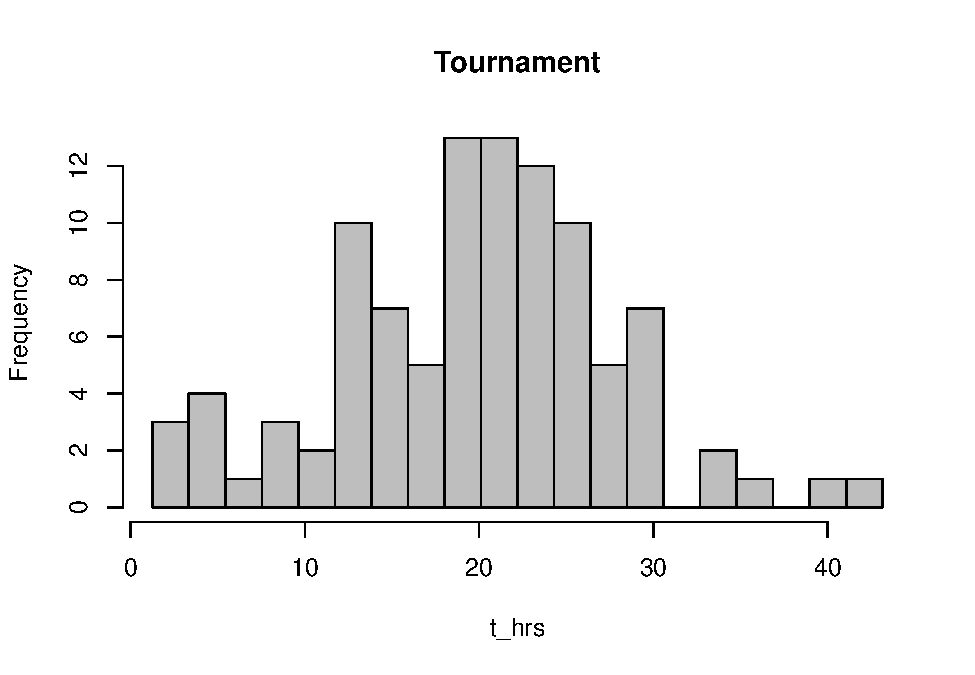
\includegraphics{au-r-workshop_files/figure-latex/unnamed-chunk-92-1} \end{center}

Notice that you need to be careful about the order of how you specify
which \texttt{lty} and \texttt{pch} settings match up with the elements
of the \texttt{legend} argument. In the \texttt{plot\ code}, you
specified that the \texttt{lty\ =\ 2} but didn't specify what
\texttt{pch} should be (it defaults to \texttt{1}). So when you put the
``Tournament'' group first the the \texttt{legend} argument vector, you
must be sure to use the corresponding plotting codes. The first element
of the \texttt{lty} argument matches up with the first element of
\texttt{legend}, and so on. There are a few other plotting tricks used:
changing the margins using \texttt{par(mar)} and the rotation of y-axis
tick mark labels using \texttt{las\ =\ 1}.

\section{Exporting Plots}\label{exporting-plots}

There are two main ways to save plots. First is a quick-and-dirty method
that saves the plots, but they are not high-resolution. The second
method produces cleaner-looking high-resolution plots.

\subsection{First Method (Click Save)}\label{first-method-click-save}

\begin{itemize}
\item
  If your plot is in the RStudio built-in graphics device: Right above
  the plot, click \emph{Export \textgreater{} Save as Image}. Change the
  name, dimensions and file type.
\item
  If your plot is in a plotting device window (opened with
  \texttt{windows()} or \texttt{quartz()}: Simply go to \emph{File
  \textgreater{} Save}.
\end{itemize}

All plots will be saved in the working directory by default. You can
also just copy the plot to your clipboard (File \textgreater{} Copy to
the clipboard \textgreater{} bitmap) and paste it where you want.

\subsection{Second Method (Use a function to dump in a new
file)}\label{second-method-use-a-function-to-dump-in-a-new-file}

If you are producing plots for a final report or publication, you want
the output to be as clean-looking as possible. You can save
high-resolution plots through R by using the following steps:

\begin{Shaded}
\begin{Highlighting}[]
\CommentTok{# step 1: Make a pixels per inch object}
\NormalTok{ppi =}\StringTok{ }\DecValTok{600}

\CommentTok{# step 2: Call the figure file creation function}
\KeywordTok{png}\NormalTok{(}\StringTok{"TestFigure.png"}\NormalTok{, }\DataTypeTok{h =} \DecValTok{8} \OperatorTok{*}\StringTok{ }\NormalTok{ppi, }\DataTypeTok{w =} \DecValTok{8} \OperatorTok{*}\StringTok{ }\NormalTok{ppi, }\DataTypeTok{res =}\NormalTok{ ppi)}

\CommentTok{# step 3: Run the plot }
\CommentTok{# put all of your plotting code here (without windows())}

\CommentTok{# step 4: Close the device}
\KeywordTok{dev.off}\NormalTok{()}
\end{Highlighting}
\end{Shaded}

A plot will be saved in your working directory containing the plot made
by the code in step 3 above. The \texttt{ppi} object is pixels-per-inch.
When you specify \texttt{h\ =\ 8\ *\ ppi}, you are saying ``make a plot
with height equal to 8 inches''. There are similar functions to make
PDFs, tiff files, jpegs, etc.

\section{Bonus Topic: Error Bars}\label{bonus-topic-error-bars}

Rarely do we ever present estimates without some measure of uncertainty.
The most common way for visualizing the uncertainty in an estimate is by
using error bars. Error bars can be added to a plot using the
\texttt{arrows} function. For \texttt{arrows}, you need:

\begin{itemize}
\tightlist
\item
  Vectors of the \texttt{x} and \texttt{y} coordinates of the lower
  bound of the error bar
\item
  Vectors of the \texttt{x} and \texttt{y} coordinates of the upper
  bound of the error bar
\end{itemize}

The syntax for \texttt{arrows} is as follows:
\texttt{arrows(x0,\ y0,\ x1,\ y1,\ ...)}, where \texttt{x0} and
\texttt{y0} are the coordinates you are drawing ``from'' (e.g., lower
limits) and the \texttt{x1} and \texttt{y1} are the coordinates you are
drawing ``to'' (e.g., upper limits). The \texttt{...} represents other
arguments to change how the error bars look. Let's use a simple example.
Calculate the mean and standard deviations of the different fishery
sectors (remember how \texttt{tapply} works?):

Create error bars on the following graph:

\begin{Shaded}
\begin{Highlighting}[]
\NormalTok{x_bar =}\StringTok{ }\KeywordTok{tapply}\NormalTok{(dat}\OperatorTok{$}\NormalTok{hours, dat}\OperatorTok{$}\NormalTok{fishery, mean)}
\KeywordTok{barplot}\NormalTok{(x_bar)}
\end{Highlighting}
\end{Shaded}

\begin{center}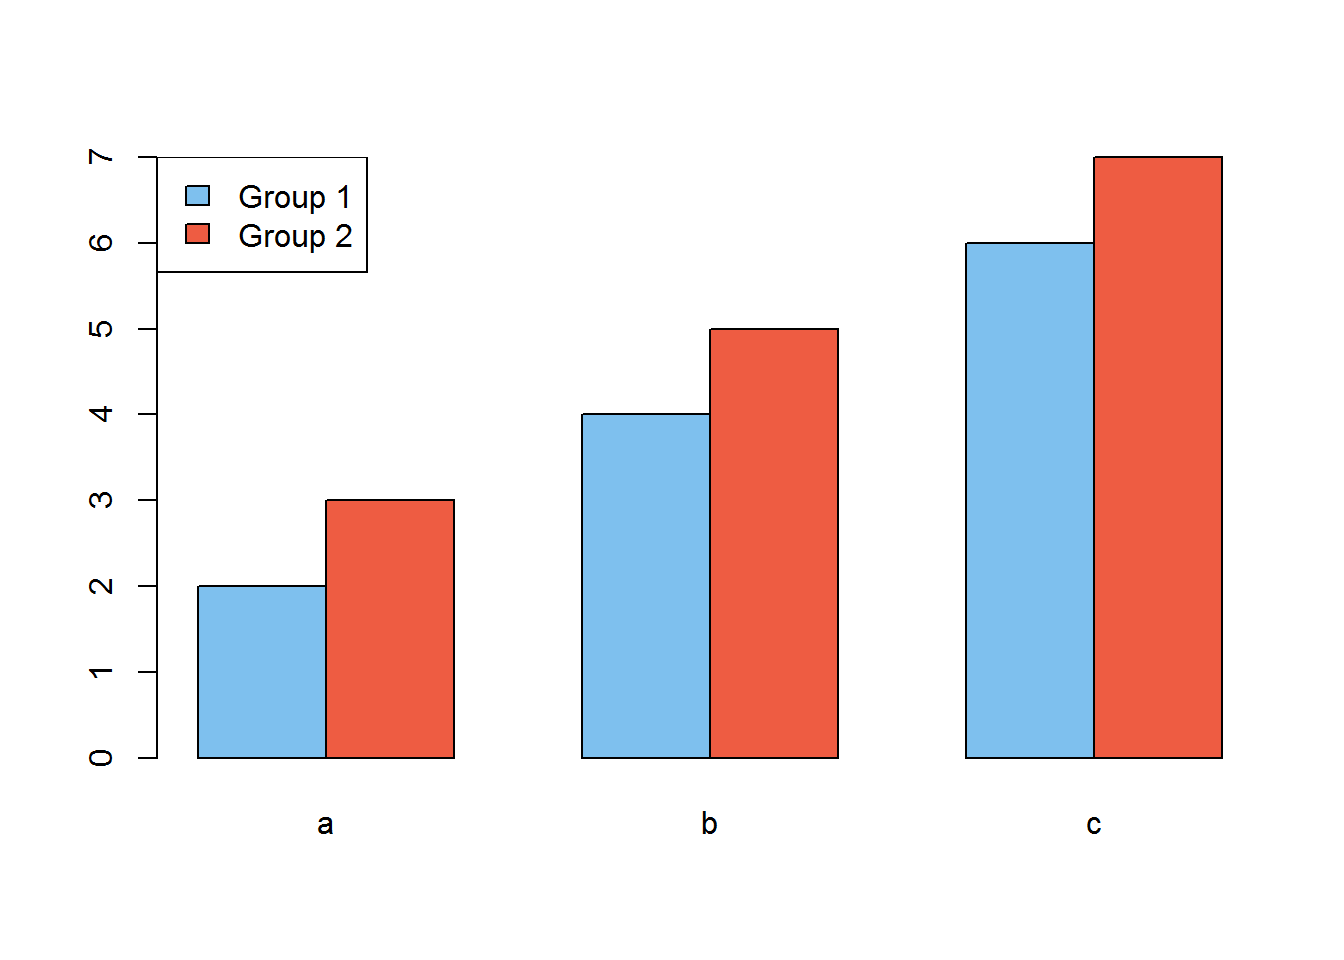
\includegraphics{au-r-workshop_files/figure-latex/unnamed-chunk-94-1} \end{center}

where the error bars represent 95\% confidence intervals on the mean.
You can create a 95\% confidence interval using this basic formula:

\[ \bar{x} \pm 1.96 * SE(\bar{x}) \]

where

\[\bar{x}=\frac{1}{n}\sum_i^n{x_i}\]

and

\[SE(\bar{x})=\sqrt{\frac{\sum_i^n{(x_i - \bar{x})^2}}{n - 1}}\]

Begin by creating a function to calculate the standard error
(\(SE(\bar{x})\)):

\begin{Shaded}
\begin{Highlighting}[]
\NormalTok{calc_se =}\StringTok{ }\ControlFlowTok{function}\NormalTok{(x) \{}
  \KeywordTok{sqrt}\NormalTok{(}\KeywordTok{sum}\NormalTok{((x }\OperatorTok{-}\StringTok{ }\KeywordTok{mean}\NormalTok{(x))}\OperatorTok{^}\DecValTok{2}\NormalTok{)}\OperatorTok{/}\NormalTok{(}\KeywordTok{length}\NormalTok{(x) }\OperatorTok{-}\StringTok{ }\DecValTok{1}\NormalTok{))}
\NormalTok{\}}
\end{Highlighting}
\end{Shaded}

Then calculate the standard errors for each fishery type:

\begin{Shaded}
\begin{Highlighting}[]
\NormalTok{se =}\StringTok{ }\KeywordTok{tapply}\NormalTok{(dat}\OperatorTok{$}\NormalTok{hours, dat}\OperatorTok{$}\NormalTok{fishery, calc_se)}
\end{Highlighting}
\end{Shaded}

Then calculate the lower and upper limits of your bars:

\begin{Shaded}
\begin{Highlighting}[]
\NormalTok{lwr =}\StringTok{ }\NormalTok{x_bar }\OperatorTok{-}\StringTok{ }\FloatTok{1.96} \OperatorTok{*}\StringTok{ }\NormalTok{se}
\NormalTok{upr =}\StringTok{ }\NormalTok{x_bar }\OperatorTok{+}\StringTok{ }\FloatTok{1.96} \OperatorTok{*}\StringTok{ }\NormalTok{se}
\end{Highlighting}
\end{Shaded}

Then draw them on using the arrows function:

\begin{Shaded}
\begin{Highlighting}[]
\NormalTok{mp =}\StringTok{ }\KeywordTok{barplot}\NormalTok{(x_bar, }\DataTypeTok{ylim =} \KeywordTok{range}\NormalTok{(}\KeywordTok{c}\NormalTok{(lwr, upr)))}
\KeywordTok{arrows}\NormalTok{(}\DataTypeTok{x0 =}\NormalTok{ mp, }\DataTypeTok{y0 =}\NormalTok{ lwr, }\DataTypeTok{x1 =}\NormalTok{ mp, }\DataTypeTok{y1 =}\NormalTok{ upr, }\DataTypeTok{length =} \FloatTok{0.1}\NormalTok{, }\DataTypeTok{angle =} \DecValTok{90}\NormalTok{, }\DataTypeTok{code =} \DecValTok{3}\NormalTok{)}
\end{Highlighting}
\end{Shaded}

\begin{center}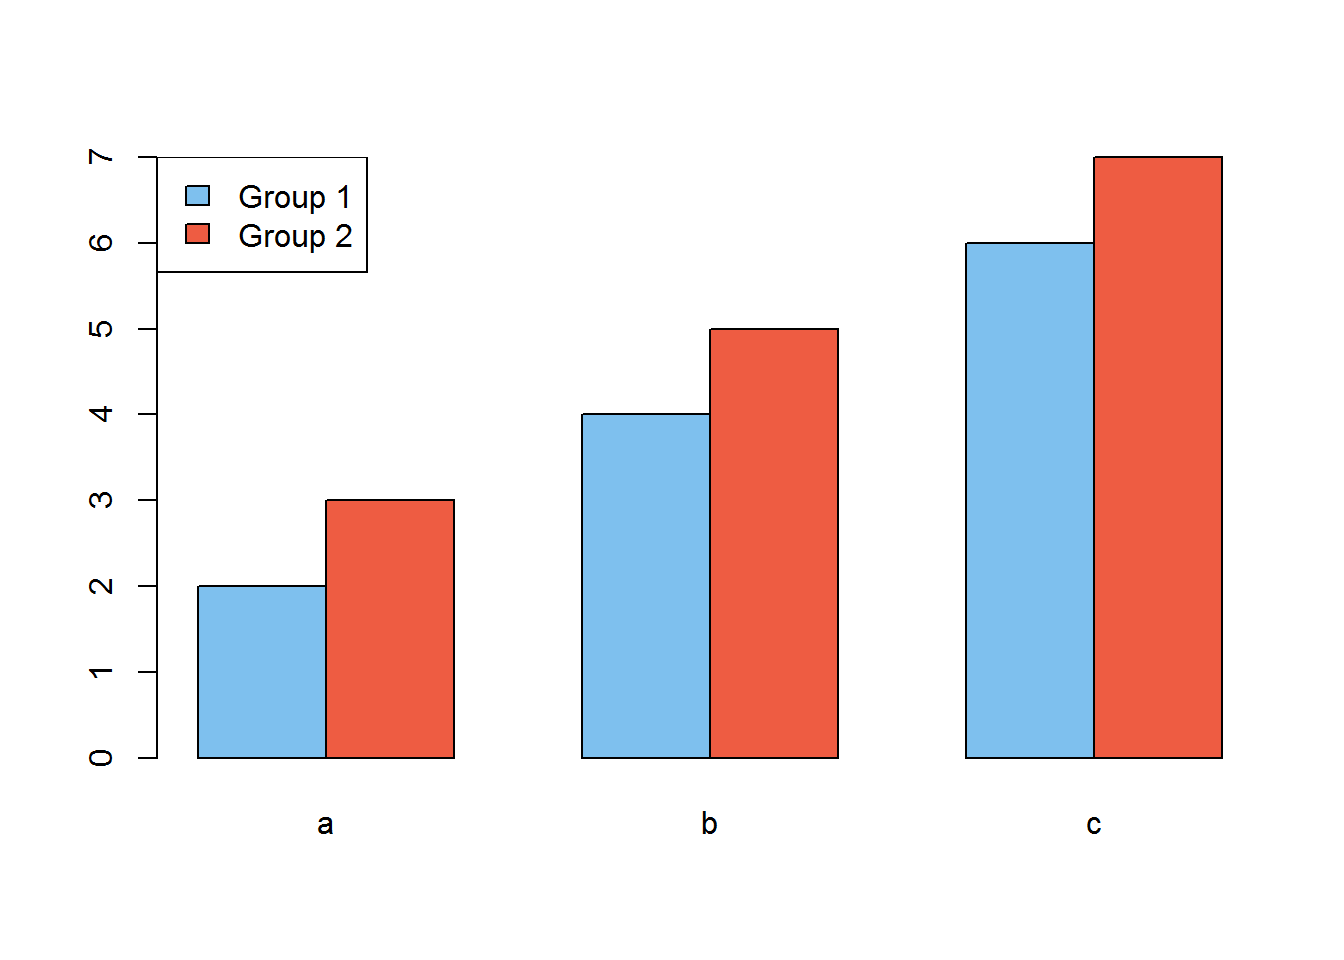
\includegraphics{au-r-workshop_files/figure-latex/unnamed-chunk-98-1} \end{center}

Notice four things:

\begin{itemize}
\item
  The use of \texttt{mp} to specify the \texttt{x} coordinate. If you do
  \texttt{mp\ =\ barplot(...)}, \texttt{mp} will contain the \texttt{x}
  coordinates of the midpoint of each bar.
\item
  \texttt{x0} and \texttt{x1} are the same: you wish to have vertical
  bars, so these must be the same while \texttt{y1} and \texttt{y2}
  differ.
\item
  The use of \texttt{ylim\ =\ range(c(lwr,\ upr))}: you want the y-axis
  to show the full range of all the error bars.
\item
  The three arguments at the end of \texttt{arrows}:

  \begin{itemize}
  \tightlist
  \item
    \texttt{length\ =\ 0.1}: the length of the arrow heads, fiddle with
    this until you like it.
  \item
    \texttt{angle\ =\ 90}: the angle of the arrow heads, you want 90
    here for the error bars.
  \item
    \texttt{code\ =\ 3}: indicates that arrow heads should be drawn on
    both ends of the arrow.
  \end{itemize}
\end{itemize}

\section*{EXERCISE 2}\label{exercise-2}
\addcontentsline{toc}{section}{EXERCISE 2}

For this exercise, you will be making a few of plots and changing how
they look to suit your taste. You will use a real dataset this time from
a sockeye salmon (\emph{Oncorhynchus nerka}) population from the
Columbia/Snake River system. This population spawns in Redfish Lake in
Idaho, which feeds into the Salmon River which is a tributary of the
Snake River. In order to reach the lake, the sockeye salmon must
successfully pass through a total eight dams that have fish passage
mechanisms in place. The Redfish Lake population is one of the most
endangered sockeye populations in the U.S. and travels farther (1,448
km), higher (1,996 m), and is the southernmost population of all sockeye
populations in the world (Kline and Flagg 2014). Given this uniqueness,
a captive breeding program was initiated in 1991 to preserve the genes
from this population. These data came from both hatchery-raised and wild
fish and include average female spawner weight (g), fecundity (number of
eggs), egg size (eggs/g), and \% survival to the eyed-egg stage.

\begin{enumerate}
\def\labelenumi{\arabic{enumi}.}
\item
  Create a new R script called \texttt{Ex2.R} and save it in the
  \texttt{Chapter2} directory. Download the \texttt{sockeye.csv} data
  set from GitHub and read it into R. Produce a basic summary of the
  data and take note of the data classes, missing values (\texttt{NA}),
  and the relative ranges for each variable.
\item
  Make a histogram of fish weights for only hatchery-origin fish. Set
  \texttt{breaks\ =\ 10} so you can see the distribution more clearly.
\item
  Make a scatter plot of the fecundity of females as a function of their
  body weight for wild fish only. Use whichever plotting character
  (\texttt{pch}) and color (\texttt{col}) you wish. Change the main
  title and axes labels to reflect what they mean. Change the x-axis
  limits to be 600 to 3000 and the y-axis limits to be 0 to 3500.
  (\emph{Hint: The \texttt{NAs} will not cause a problem. R will only
  use points where there is data for both \texttt{x} and \texttt{y} and
  ignore otherwise}).
\item
  Add points that do the same thing but for hatchery fish. Use a
  different plotting character and a different color.
\item
  Add a legend to the plot to differentiate between the two types of
  fish.
\item
  Make a multi-panel plot in a new window with box-and-whisker plots
  that compare (1) spawner weight, (2) fecundity, and (3) egg size
  between hatchery and wild fish. (\emph{Hint: each comparison will be
  on its own panel}). Change the titles of each plot to reflect what you
  are comparing.
\item
  Save the plot as a .png file in your working directory with a file
  name of your choosing.
\end{enumerate}

\subsection{EXERCISE 2 BONUS}\label{exercise-2-bonus}

\begin{enumerate}
\def\labelenumi{\arabic{enumi}.}
\item
  Make a bar plot comparing the mean survival to eyed-egg stage for each
  type of fish (hatchery and wild). Add error bars that represent +/-
  2SE of each mean.
\item
  Change the names of each bar, the main plot title, and the y-axis
  title.
\end{enumerate}

\textbf{Reference for data} Kline, P.A. and T.A. Flagg. 2014. Putting
the red back in Redfish Lake, 20 years of progress toward saving the
Pacific Northwest's most endangered salmon population.
\textbf{Fisheries}. \emph{39(11)}: 488-500.

\chapter{Basic Statistics}\label{ch3}

\section*{Chapter Overview}\label{chapter-overview-2}
\addcontentsline{toc}{section}{Chapter Overview}

In this chapter, you will get familiar with the basics of using R for
the purpose it was designed: statisitical analysis. You will learn how
to:

\begin{itemize}
\tightlist
\item
  how to fit and interpret the output from various general linear
  models:

  \begin{itemize}
  \tightlist
  \item
    simple linear regression models
  \item
    multiple regression models
  \item
    higher order polynomial regression models
  \item
    T-tests (also ANOVA)
  \item
    ANCOVA models
  \item
    Interactions
  \end{itemize}
\item
  very basic model selection
\item
  basic GLMs: the logistic regression model
\item
  Bonus topic: fitting non-linear regression models using \texttt{nls}
\item
  Bonus topic: fitting custom maximum-likelihood models using
  \texttt{optim}
\end{itemize}

R's built-in statistical modeling framework is pretty intuitive and
comprehensive. R has gained popularity as a statistics software and is
commonly used both in academia and governmental resource agencies. This
popularity is likely a result of its power, flexibility, intuitive
nature, and price (free!). For many students, this chapter may be the
one that is most immediately useful.

\textbf{IMPORTANT NOTE}: If you did not attend the sessions
corresponding to Chapters \ref{ch1} or \ref{ch2}, you are recommended to
walk through the material found in those chapters before proceeding to
this material. Also note that if you are confused about a topic, you can
use \textbf{CTRL + F} to find previous cases where that topic has been
discussed in this document.

\section*{Before You Begin}\label{before-you-begin-1}
\addcontentsline{toc}{section}{Before You Begin}

You should create a new directory and R script for your work in this
Chapter. Create a new R script called \texttt{Ch3.R} and save it in the
directory \texttt{C:/Users/YOU/Documents/R-Workshop/Chapter3}. Set your
working directory to that location. Revisit the material in Sections
\ref{scripts} and \ref{working-dir} for more details on these steps.

\section{Review: The General Linear
Model}\label{review-the-general-linear-model}

This is a family of models that allows you to determine the relationship
(if any) between some continuous response variable (\(y\)) and some
predictor variable(s) (\(x_n\)) and is often written as:

\[y_i=\beta_0 + \beta_1 x_{i1} + ... + \beta_j x_{ij}+ ... + \beta_n x_{in} + \varepsilon_i; \varepsilon_i \sim N(0,\sigma)\]

The predictor variable(s) can be either categorical (i.e., grouping
variables used in ANOVA, t-test, etc.), continuous (regression), or a
combination of categorical and continuous (ANCOVA). The main focus is to
estimate the coefficients (\(\beta\)), and in some cases it is to
determine if they are ``significantly'' different from the value given
by some null hypothesis.

The model makes several assumptions about the residuals\footnote{The
  residuals (\(\varepsilon_i\)) are the difference between the data
  point \(y_i\) and the model prediction \(\hat{y}_i\):
  \(\varepsilon_i=y_i-\hat{y}_i\)} to obtain estimates of the
coefficients. For reliable inference, the residuals must:

\begin{itemize}
\tightlist
\item
  Be independent
\item
  Be normally-distributed
\item
  Have constant variance across range of the x-axis
\end{itemize}

In R, the general linear model is fitted using the \texttt{lm} function.
Here's the basic syntax is
\texttt{lm(y\ \textasciitilde{}\ x,\ data\ =\ dat)}\footnote{This should
  look familar from Section \ref{box-whisker}}; it says: ``fit a model
with \texttt{y} as the response variable and \texttt{x} as the sole
predictor variable, look for the variables \texttt{x} and \texttt{y} in
a data frame called \texttt{dat}, and store the results in a new object
called \texttt{fit}''.

\section{Simple Linear Regression}\label{regression}

Download the data set \texttt{sockeye.csv} from GitHub and place it in
your working directory. This is the same data set you used in Exercise
2, see that section for more details on the different variables.

Read these data into R:

\begin{Shaded}
\begin{Highlighting}[]
\NormalTok{dat =}\StringTok{ }\KeywordTok{read.csv}\NormalTok{(}\StringTok{"sockeye.csv"}\NormalTok{)}
\KeywordTok{head}\NormalTok{(dat)}
\end{Highlighting}
\end{Shaded}

\begin{verbatim}
##   year  type weight fecund egg_size survival
## 1 1991 hatch     NA     NA       NA       NA
## 2 1992 hatch     NA     NA       NA       NA
## 3 1993 hatch   1801   2182    12.25    46.58
## 4 1994 hatch   1681   2134     7.92    50.98
## 5 1995 hatch   2630   1576    21.61    68.06
## 6 1996 hatch   2165   2171     8.74    63.43
\end{verbatim}

To fit a regression model using \texttt{lm}, but \texttt{x} and
\texttt{y} must be continous (numeric) variables. In the data set
\texttt{dat}, two such variables are the \texttt{weight} and
\texttt{fecund}. Fit a regression model where you link the average
fecundity of an individual to the average weight of an individual by
treating years as replicate data points. Ignore for now that the fish
come from two sources: hatchery and wild origin.

\begin{Shaded}
\begin{Highlighting}[]
\NormalTok{fit1 =}\StringTok{ }\KeywordTok{lm}\NormalTok{(fecund }\OperatorTok{~}\StringTok{ }\NormalTok{weight, }\DataTypeTok{data =}\NormalTok{ dat)}
\end{Highlighting}
\end{Shaded}

If you run just the \texttt{fit1} object, you will see the model you ran
along with the coefficient estimates of the intercept (\(\beta_0\)) and
the slope (\(\beta_1\)):

\begin{Shaded}
\begin{Highlighting}[]
\NormalTok{fit1}
\end{Highlighting}
\end{Shaded}

\begin{verbatim}
## 
## Call:
## lm(formula = fecund ~ weight, data = dat)
## 
## Coefficients:
## (Intercept)       weight  
##   1874.6496       0.2104
\end{verbatim}

If \(x_{i1}\) is \texttt{weight}, then the coefficients are interpretted
as:

\begin{itemize}
\tightlist
\item
  \(\beta_0\): the y-intercept (mean \texttt{fecund} at zero
  \texttt{weight})
\item
  \(\beta_1\): the slope (change in \texttt{fecund} for one unit
  increase in \texttt{weight})
\end{itemize}

For more information about the model fit, you can use the
\texttt{summary} function:

\begin{Shaded}
\begin{Highlighting}[]
\KeywordTok{summary}\NormalTok{(fit1)}
\end{Highlighting}
\end{Shaded}

\begin{verbatim}
## 
## Call:
## lm(formula = fecund ~ weight, data = dat)
## 
## Residuals:
##     Min      1Q  Median      3Q     Max 
## -873.67 -389.28  -71.65  482.96 1041.24 
## 
## Coefficients:
##              Estimate Std. Error t value Pr(>|t|)    
## (Intercept) 1874.6496   269.4369   6.958 4.33e-08 ***
## weight         0.2104     0.1803   1.167    0.251    
## ---
## Signif. codes:  0 '***' 0.001 '**' 0.01 '*' 0.05 '.' 0.1 ' ' 1
## 
## Residual standard error: 500.6 on 35 degrees of freedom
##   (7 observations deleted due to missingness)
## Multiple R-squared:  0.03745,    Adjusted R-squared:  0.009945 
## F-statistic: 1.362 on 1 and 35 DF,  p-value: 0.2511
\end{verbatim}

Again the coefficient estimates are shown, but now you see the
uncertainty on the parameter estimates (standard errors), the test
statistic, and the p-value testing the null hypothesis that each
coefficient has a zero value. Here you can see that the p-value does not
support rejection of the null hypothesis that the slope is zero. You can
see the residual standard error (variability of data around the line and
the estimate of \(\sigma\)), the \(R^2\) value (the proportion of
variation in \texttt{fecund} explained by variation in \texttt{weight}),
and the p-value of the overall model.

You can easily see the model fit by using the \texttt{abline} function.
Make a new plot and add the fitted regression line:

\begin{Shaded}
\begin{Highlighting}[]
\KeywordTok{plot}\NormalTok{(fecund }\OperatorTok{~}\StringTok{ }\NormalTok{weight, }\DataTypeTok{data =}\NormalTok{ dat, }\DataTypeTok{col =} \StringTok{"grey"}\NormalTok{, }\DataTypeTok{pch =} \DecValTok{16}\NormalTok{, }\DataTypeTok{cex =} \FloatTok{1.5}\NormalTok{)}
\KeywordTok{abline}\NormalTok{(fit1)}
\end{Highlighting}
\end{Shaded}

\begin{center}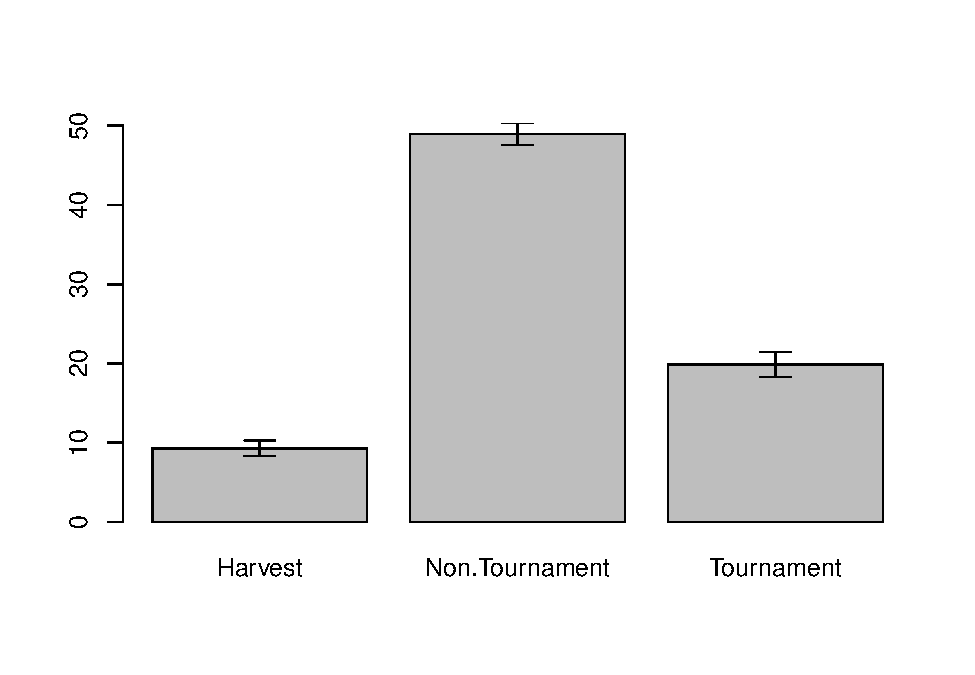
\includegraphics{au-r-workshop_files/figure-latex/unnamed-chunk-105-1} \end{center}

It fits, but not very well. It seems there are two groups: one with data
points mostly above the line and one with data points mostly below the
line. You'll now run a new model to get at this.

\section{ANOVA: Categorical predictors}\label{anova}

ANOVA models attempt to determine if the means of different groups are
different. You can fit them in the same basic \texttt{lm} framework. But
first, notice that:

\begin{Shaded}
\begin{Highlighting}[]
\KeywordTok{class}\NormalTok{(dat}\OperatorTok{$}\NormalTok{type); }\KeywordTok{levels}\NormalTok{(dat}\OperatorTok{$}\NormalTok{type)}
\end{Highlighting}
\end{Shaded}

\begin{verbatim}
## [1] "factor"
\end{verbatim}

\begin{verbatim}
## [1] "hatch" "wild"
\end{verbatim}

tells you the \texttt{type} variable is a factor. It has levels of
\texttt{"hatch"} and \texttt{"wild"} which indicate the origin of the
adult spawning fish sampled each year. If you pass \texttt{lm} a
predictor variable with a factor class, the R will automatically fit it
as an ANOVA model. See Section \ref{factors} for more details on
factors. Factors have an explicit ordering of the levels. By default,
this ordering happens alphabetically: if your factor has levels
\texttt{"a"}, \texttt{"b"}, and \texttt{"c"}, they will be assigned the
order of \texttt{1}, \texttt{2} and \texttt{3}, respectively. You can
always see how R is ordering your factor by doing something similar to
this:

\begin{Shaded}
\begin{Highlighting}[]
\NormalTok{pairs =}\StringTok{ }\KeywordTok{cbind}\NormalTok{(}
  \KeywordTok{as.character}\NormalTok{(dat}\OperatorTok{$}\NormalTok{type),}
  \KeywordTok{as.numeric}\NormalTok{(dat}\OperatorTok{$}\NormalTok{type)}
\NormalTok{)}

\KeywordTok{head}\NormalTok{(pairs); }\KeywordTok{tail}\NormalTok{(pairs)}
\end{Highlighting}
\end{Shaded}

\begin{verbatim}
##      [,1]    [,2]
## [1,] "hatch" "1" 
## [2,] "hatch" "1" 
## [3,] "hatch" "1" 
## [4,] "hatch" "1" 
## [5,] "hatch" "1" 
## [6,] "hatch" "1"
\end{verbatim}

\begin{verbatim}
##       [,1]   [,2]
## [39,] "wild" "2" 
## [40,] "wild" "2" 
## [41,] "wild" "2" 
## [42,] "wild" "2" 
## [43,] "wild" "2" 
## [44,] "wild" "2"
\end{verbatim}

The functions \texttt{as.character} and \texttt{as.numeric} are coersion
functions: they attempt to change the way something is interpretted.
Notice that the level \texttt{"hatch"} is assigned the order \texttt{1}
because it comes before \texttt{"wild"} alphebetically. The first level
is termed the \textbf{reference level} because it is the group that all
other levels are compared to when fitting a model. You can change the
reference level using
\texttt{dat\$type\_rlvl\ =\ relevel(dat\$type,\ ref\ =\ "wild")}.

You are now ready to fit the ANOVA model, which will measure the size of
the difference in the mean \texttt{fecund} between different levels of
the factor \texttt{type}:

\begin{Shaded}
\begin{Highlighting}[]
\NormalTok{fit2 =}\StringTok{ }\KeywordTok{lm}\NormalTok{(fecund }\OperatorTok{~}\StringTok{ }\NormalTok{type, }\DataTypeTok{data =}\NormalTok{ dat)}
\end{Highlighting}
\end{Shaded}

Think of this model as being written as:

\[y_i=\beta_0 + \beta_1 x_{i1} + \varepsilon_i\] and assume that
\(x_{i1} = 0\) if observation \(i\) is from \texttt{"hatch"} fish and
\(x_{i1} = 1\) if observation \(i\) is from \texttt{"wild"} fish. In
that case:

\begin{itemize}
\tightlist
\item
  \(\beta_0\) (the intercept) is interpretted as the mean
  \texttt{fecund} for the \texttt{"hatch"} level and
\item
  \(\beta_1\) is interpretted as the difference in mean \texttt{fecund}
  between the \texttt{"wild"} level and the \texttt{"hatch"} level.
\end{itemize}

So when you run \texttt{coef(fit2)} to extract the coefficient estimates
and get:

\begin{verbatim}
## (Intercept)    typewild 
##   1846.2500    713.3971
\end{verbatim}

you see that the mean fecundity of hatchery fish is about 1846 eggs and
that the average wild fish has about 713 more eggs than the average
hatchery fish across all years. The fact that the p-value associated
with the \texttt{typewild} coefficient when you run
\texttt{summary(fit2)} is less than 0.05 indicates that there is
statistical evidence that the difference in means is not zero.

\section{ANCOVA: Continuous and categorical
predictors}\label{ancova-continuous-and-categorical-predictors}

Now that you have seen that hatchery and wild fish tend to separate
along the fecundity axis (as evidenced by the ANOVA results above), you
would like to include this in your original regression model. You will
fit two lines within the same model: one for hatchery fish and one for
wild fish. This model is called an ANCOVA model and looks like this:

\[y_i=\beta_0 + \beta_1 x_{i1} + \beta_2 x_{i2} + \varepsilon_i\]

If \(x_{i1}\) is \texttt{type} coded with 0's and 1's as in Section
\ref{anova} and \(x_{i2}\) is \texttt{weight}, then the coefficients are
interpretted as:

\begin{itemize}
\tightlist
\item
  \(\beta_0\): the y-intercept of the \texttt{"hatch"} level (the
  reference level)
\item
  \(\beta_1\): the difference in y-intercept between the \texttt{"wild"}
  level and the \texttt{"hatch"} level.
\item
  \(\beta_2\): the slope of both lines (this model assumes the lines
  have common slopes, i.e., that the lines are parallel)
\end{itemize}

You can fit this model and extract the coefficents table from the
summary:

\begin{Shaded}
\begin{Highlighting}[]
\NormalTok{fit3 =}\StringTok{ }\KeywordTok{lm}\NormalTok{(fecund }\OperatorTok{~}\StringTok{ }\NormalTok{type }\OperatorTok{+}\StringTok{ }\NormalTok{weight, }\DataTypeTok{data =}\NormalTok{ dat)}
\KeywordTok{summary}\NormalTok{(fit3)}\OperatorTok{$}\NormalTok{coef}
\end{Highlighting}
\end{Shaded}

\begin{verbatim}
##                 Estimate  Std. Error  t value     Pr(>|t|)
## (Intercept) 1039.6417645 175.0992184 5.937444 1.038268e-06
## typewild     866.9909998  96.2473387 9.007948 1.578239e-10
## weight         0.5173716   0.1051039 4.922477 2.164460e-05
\end{verbatim}

And you can plot the fit. Study this code to make sure you know what
each is doing. Use what you know about the meanings of the three
coefficients to decipher the two \texttt{abline} commands. Remember that
\texttt{abline} takes takes two arguments: \texttt{a} is the intercept
and \texttt{b} is the slope.

\begin{Shaded}
\begin{Highlighting}[]
\KeywordTok{plot}\NormalTok{(fecund }\OperatorTok{~}\StringTok{ }\NormalTok{weight, }\DataTypeTok{data =}\NormalTok{ dat, }\DataTypeTok{col =} \StringTok{"grey"}\NormalTok{,}
     \DataTypeTok{pch =} \KeywordTok{ifelse}\NormalTok{(dat}\OperatorTok{$}\NormalTok{type }\OperatorTok{==}\StringTok{ "hatch"}\NormalTok{, }\DecValTok{1}\NormalTok{, }\DecValTok{16}\NormalTok{), }\DataTypeTok{cex =} \FloatTok{1.5}\NormalTok{)}
\KeywordTok{abline}\NormalTok{(}\KeywordTok{coef}\NormalTok{(fit3)[}\KeywordTok{c}\NormalTok{(}\DecValTok{1}\NormalTok{,}\DecValTok{3}\NormalTok{)], }\DataTypeTok{lty =} \DecValTok{2}\NormalTok{)}
\KeywordTok{abline}\NormalTok{(}\KeywordTok{sum}\NormalTok{(}\KeywordTok{coef}\NormalTok{(fit3)[}\KeywordTok{c}\NormalTok{(}\DecValTok{1}\NormalTok{,}\DecValTok{2}\NormalTok{)]), }\KeywordTok{coef}\NormalTok{(fit3)[}\DecValTok{3}\NormalTok{])}
\KeywordTok{legend}\NormalTok{(}\StringTok{"bottom"}\NormalTok{, }\DataTypeTok{legend =} \KeywordTok{c}\NormalTok{(}\StringTok{"Hatchery"}\NormalTok{, }\StringTok{"Wild"}\NormalTok{), }\DataTypeTok{pch =} \KeywordTok{c}\NormalTok{(}\DecValTok{1}\NormalTok{,}\DecValTok{16}\NormalTok{), }\DataTypeTok{lty =} \KeywordTok{c}\NormalTok{(}\DecValTok{2}\NormalTok{,}\DecValTok{1}\NormalTok{),}
       \DataTypeTok{col =} \StringTok{"grey"}\NormalTok{, }\DataTypeTok{pt.cex =} \FloatTok{1.5}\NormalTok{, }\DataTypeTok{bty =} \StringTok{"n"}\NormalTok{, }\DataTypeTok{horiz =}\NormalTok{ T)}
\end{Highlighting}
\end{Shaded}

\begin{center}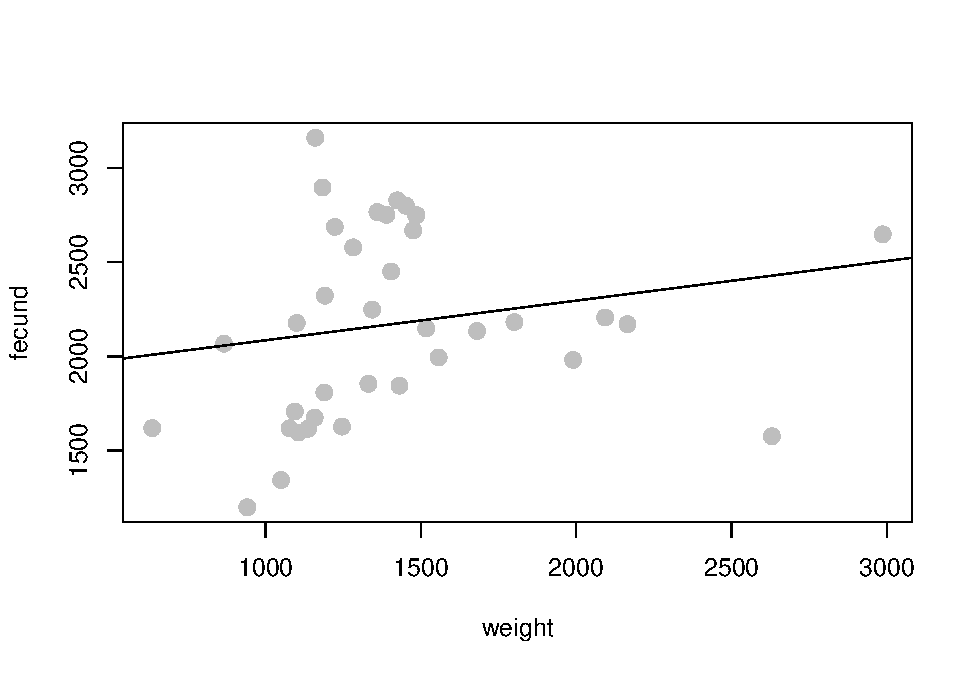
\includegraphics{au-r-workshop_files/figure-latex/unnamed-chunk-111-1} \end{center}

\section{Interactions}\label{interactions}

Above, you have included an additional predictor variable (and
parameter) in your model to help explain variation in the
\texttt{fecund} variable. However, you have assumed that the effect of
weight on fecundity is common between hatchery and wild fish (note the
parallel lines in the figure above). You may have reason to believe that
the effect of weight depends on the origin of the fish, e.g., wild fish
may tend to accumulate more eggs than hatchery fish for the same
increase in weight. Cases where the magnitude of the effect depends on
the value of another predictor variable are known as ``interactions''.
You can write the interactive ANCOVA model like this:

\[y_i=\beta_0 + \beta_1 x_{i1} + \beta_2 x_{i2} + \beta_3 x_{i1} x_{i2} + \varepsilon_i\]

If \(x_{i1}\) is \texttt{type} coded with 0's and 1's as in Section
\ref{anova} and \(x_{i2}\) is \texttt{weight}, then the coefficients are
interpretted as:

\begin{itemize}
\tightlist
\item
  \(\beta_0\): the y-intercept of the \texttt{"hatch"} level (the
  reference level)
\item
  \(\beta_1\): the difference in y-intercept between the \texttt{"wild"}
  level and the \texttt{"hatch"} level.
\item
  \(\beta_2\): the slope of the \texttt{"hatch"} level
\item
  \(\beta_3\): the difference in slope between the \texttt{"wild"} level
  and the \texttt{"hatch"} level.
\end{itemize}

You can fit this model:

\begin{Shaded}
\begin{Highlighting}[]
\NormalTok{fit4 =}\StringTok{ }\KeywordTok{lm}\NormalTok{(fecund }\OperatorTok{~}\StringTok{ }\NormalTok{type }\OperatorTok{+}\StringTok{ }\NormalTok{weight }\OperatorTok{+}\StringTok{ }\NormalTok{type}\OperatorTok{:}\NormalTok{weight, }\DataTypeTok{data =}\NormalTok{ dat)}

\CommentTok{# or}
\CommentTok{# fit4 = lm(fecund ~ type * weight, data = dat)}
\end{Highlighting}
\end{Shaded}

The first option above is more clear in its statement, but both do the
same thing.

You can plot the fit. Study these lines to make sure you know what each
is doing. Use what you know about the meanings of the four coefficients
to decipher the two \texttt{abline} commands.

\begin{Shaded}
\begin{Highlighting}[]
\KeywordTok{plot}\NormalTok{(fecund }\OperatorTok{~}\StringTok{ }\NormalTok{weight, }\DataTypeTok{data =}\NormalTok{ dat, }\DataTypeTok{col =} \StringTok{"grey"}\NormalTok{,}
     \DataTypeTok{pch =} \KeywordTok{ifelse}\NormalTok{(dat}\OperatorTok{$}\NormalTok{type }\OperatorTok{==}\StringTok{ "hatch"}\NormalTok{, }\DecValTok{1}\NormalTok{, }\DecValTok{16}\NormalTok{), }\DataTypeTok{cex =} \FloatTok{1.5}\NormalTok{)}
\KeywordTok{abline}\NormalTok{(}\KeywordTok{coef}\NormalTok{(fit4)[}\KeywordTok{c}\NormalTok{(}\DecValTok{1}\NormalTok{,}\DecValTok{3}\NormalTok{)], }\DataTypeTok{lty =} \DecValTok{2}\NormalTok{)}
\KeywordTok{abline}\NormalTok{(}\KeywordTok{sum}\NormalTok{(}\KeywordTok{coef}\NormalTok{(fit4)[}\KeywordTok{c}\NormalTok{(}\DecValTok{1}\NormalTok{,}\DecValTok{2}\NormalTok{)]), }\KeywordTok{sum}\NormalTok{(}\KeywordTok{coef}\NormalTok{(fit4)[}\KeywordTok{c}\NormalTok{(}\DecValTok{3}\NormalTok{,}\DecValTok{4}\NormalTok{)]))}
\KeywordTok{legend}\NormalTok{(}\StringTok{"bottom"}\NormalTok{, }\DataTypeTok{legend =} \KeywordTok{c}\NormalTok{(}\StringTok{"Hatchery"}\NormalTok{, }\StringTok{"Wild"}\NormalTok{), }\DataTypeTok{pch =} \KeywordTok{c}\NormalTok{(}\DecValTok{1}\NormalTok{,}\DecValTok{16}\NormalTok{), }\DataTypeTok{lty =} \KeywordTok{c}\NormalTok{(}\DecValTok{2}\NormalTok{,}\DecValTok{1}\NormalTok{),}
       \DataTypeTok{col =} \StringTok{"grey"}\NormalTok{, }\DataTypeTok{pt.cex =} \FloatTok{1.5}\NormalTok{, }\DataTypeTok{bty =} \StringTok{"n"}\NormalTok{, }\DataTypeTok{horiz =}\NormalTok{ T)}
\end{Highlighting}
\end{Shaded}

\begin{center}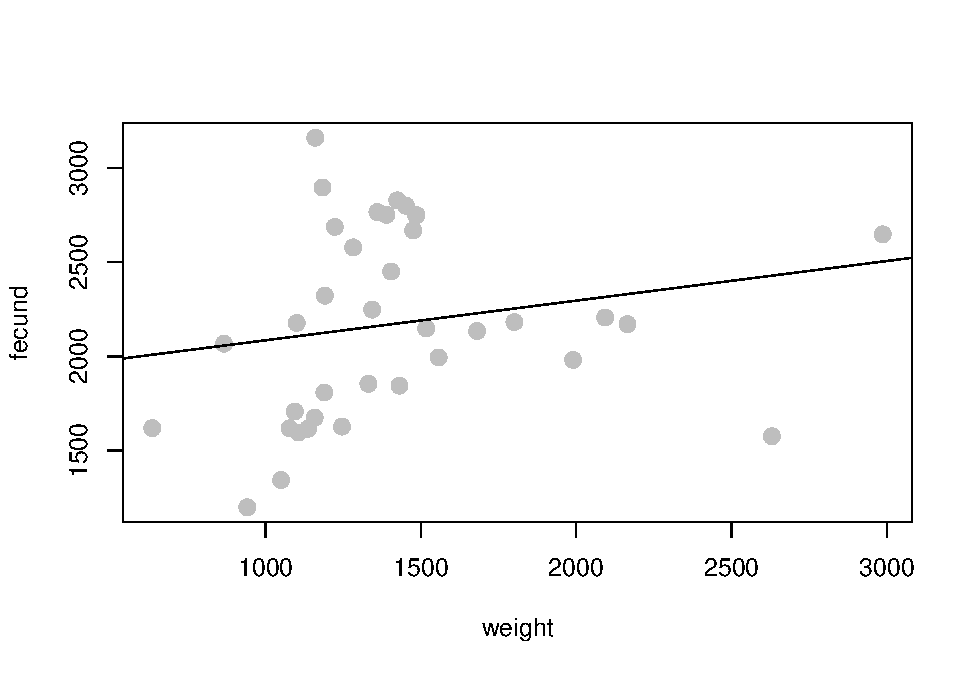
\includegraphics{au-r-workshop_files/figure-latex/unnamed-chunk-113-1} \end{center}

Based on the coefficients table:

\begin{Shaded}
\begin{Highlighting}[]
\KeywordTok{summary}\NormalTok{(fit4)}\OperatorTok{$}\NormalTok{coef}
\end{Highlighting}
\end{Shaded}

\begin{verbatim}
##                     Estimate Std. Error    t value     Pr(>|t|)
## (Intercept)     1175.7190847 174.545223  6.7358995 1.125255e-07
## typewild         -42.8721082 398.980751 -0.1074541 9.150794e-01
## weight             0.4300894   0.105592  4.0731253 2.732580e-04
## typewild:weight    0.7003389   0.299104  2.3414560 2.539681e-02
\end{verbatim}

It seems that fish of the different origins have approximately the same
intercept, but that their slopes are quite different.

\section{Model Selection: AIC}\label{model-selection-aic}

You have now fitted four different models, each that makes different
claims about how you can predict the fecundity of a given sockeye salmon
at Redfish Lake. If you are interested in determining \emph{which} of
these models you should use for prediction, you need to use
\textbf{model selection}. Model selection attempts to find the model
that is likely to have the smallest out-of-sample prediction error
(i.e., future predictions will be close to what actually happens). One
model selection metric is the AIC\footnote{Akaike's Information
  Criterion. \textbf{GIVE A CITATION HERE}}. Lower AIC values mean the
model should have better predictive performance. Compare the four models
you fitted with AIC:

\begin{Shaded}
\begin{Highlighting}[]
\KeywordTok{AIC}\NormalTok{(fit1, fit2, fit3, fit4)}
\end{Highlighting}
\end{Shaded}

\begin{verbatim}
##      df      AIC
## fit1  3 568.9166
## fit2  3 543.6914
## fit3  4 525.7834
## fit4  5 522.0968
\end{verbatim}

In general, AIC values that are different by more than 2 units are
interpretted as having importantly different predictive performance.
Based on this very quick-and-dirty analysis, it seems that in predicting
future fecundity, you would want to use the interactive ANCOVA model.

\section{An Example GLM: Logistic Regression}\label{logis-regression}

The models you fitted above were called ``general linear models''. They
all made the assumption that the residuals (\(\varepsilon_i\)) are
normally-distributed. Often times data and analyses do not follow this
assumption. For these cases you often move to the broader family of
statistical models known as ``generalized linear models''\footnote{General
  linear models are a member of this family}.

One example is in the case of \textbf{binary} data. Binary data have two
outcomes, e.g., success/failure, lived/died, male/female,
spawned/gravid, happy/sad, etc. If you wish to predict how the
probability of one outcome over the other changes depending on some
other variable, then you need to use the \textbf{logistic regression
model}, which is written as:

\[logit(p_i)=\beta_0 + \beta_1 x_{i1} + ... + \beta_j x_{ij}+ ... + \beta_n x_{in}; y_i \sim Bernoulli(p_i)\]

Where \(p_i\) is the probability that observation \(y_i\) was a success
(\(y_i = 1\)). The \(logit(p_i)\) is the \textbf{link function} that
links the linear parameter scale to the data scale. It constrains the
value of \(p_i\) to be between 0 and 1 regardless of the values of the
\(\beta\) coefficients. The logit link function does this:

\[logit(p_i) = log\left(\frac{p_i}{1-p_i}\right)\]

which is the natural logarithm of the \textbf{odds}, a measure of how
likely the event is to happen relative to it not happening. Make an R
function to calculate the logit transformation:

\begin{Shaded}
\begin{Highlighting}[]
\NormalTok{logit =}\StringTok{ }\ControlFlowTok{function}\NormalTok{(p) \{}
  \KeywordTok{log}\NormalTok{(p}\OperatorTok{/}\NormalTok{(}\DecValTok{1} \OperatorTok{-}\StringTok{ }\NormalTok{p))}
\NormalTok{\}}
\end{Highlighting}
\end{Shaded}

If you have the result of \texttt{logit(p{[}i{]})} (which is given by
the \(\beta\) coefficients and the \(x_{ij}\) data) and need to get
\texttt{p{[}i{]}}, you can apply the inverse logit function:

\[expit(lp_i)=\frac{e^{lp_i}}{1 + e^{lp_i}}\]

where \(lp_i = logit(p_i)\). Make a function for the inverse logit
transformation:

\begin{Shaded}
\begin{Highlighting}[]
\NormalTok{expit =}\StringTok{ }\ControlFlowTok{function}\NormalTok{(lp) \{  }\CommentTok{# lp stands for logit(p)}
  \KeywordTok{exp}\NormalTok{(lp)}\OperatorTok{/}\NormalTok{(}\DecValTok{1} \OperatorTok{+}\StringTok{ }\KeywordTok{exp}\NormalTok{(lp))}
\NormalTok{\}}
\end{Highlighting}
\end{Shaded}

Because of the logit link function, the coefficients have different
interpretations than in the previous models you've fitted in this
chapter: they are expressed in terms of log odds.

Fit a logistic regression model to the sockeye salmon data. None of the
variables of interest are binary, but you can create one. Look at the
variable \texttt{dat\$survival}. This is the average \% survival of all
eggs laid that make it to the ``eye-egg'' stage. Create a new variable
\texttt{binary} which takes on a 0 if \texttt{dat\$survival} is less
than 70\% and a 1 otherwise:

\begin{Shaded}
\begin{Highlighting}[]
\NormalTok{dat}\OperatorTok{$}\NormalTok{binary =}\StringTok{ }\KeywordTok{ifelse}\NormalTok{(dat}\OperatorTok{$}\NormalTok{survival }\OperatorTok{<}\StringTok{ }\DecValTok{70}\NormalTok{, }\DecValTok{0}\NormalTok{, }\DecValTok{1}\NormalTok{)}
\end{Highlighting}
\end{Shaded}

This will be your response variable and your model will estimate how the
probability of \texttt{binary} being a \texttt{1} changes (or doesn't)
depending on the value of other variables.

A basic model would have just \texttt{weight} as the predictor variable:

\begin{Shaded}
\begin{Highlighting}[]
\NormalTok{fit1 =}\StringTok{ }\KeywordTok{glm}\NormalTok{(binary }\OperatorTok{~}\StringTok{ }\NormalTok{weight, }\DataTypeTok{data =}\NormalTok{ dat, }\DataTypeTok{family =}\NormalTok{ binomial)}
\KeywordTok{summary}\NormalTok{(fit1)}\OperatorTok{$}\NormalTok{coef}
\end{Highlighting}
\end{Shaded}

\begin{verbatim}
##                 Estimate Std. Error   z value   Pr(>|z|)
## (Intercept)  4.363441330 1.76943946  2.466002 0.01366306
## weight      -0.002819271 0.00125243 -2.251040 0.02438303
\end{verbatim}

The coefficients are interpretted as:

\begin{itemize}
\item
  \(\beta_0\): the log odds of success for a fish with zero weight
  (which is not all that important). \(e^{\beta_0}\) is the odds of
  success for fish with zero weight, and \(expit(e^{\beta_0})\) is the
  probability of success for fish with zero weight. Remember ``success''
  is defined as having at least 70\% egg survival to the stage of
  interest.
\item
  \(\beta_1\): the additive effect of fish weight on the log odds of
  success. \(e^{\beta_1}\) is interpretted as the ratio of the odds at
  two consective weights (e.g., 1500 and 1501). Claims about
  \(e^{\beta_1}\) are made as ``for every one gram increase in weight,
  success became \(e^{\beta_1}\) times as likely to happen''.
\item
  You can predict the probability of success any weight using
  \(expit(\beta_0 + \beta_1 weight)\)
\end{itemize}

You can plot the fitted model:

\begin{Shaded}
\begin{Highlighting}[]
\CommentTok{# create a sequence of weights to predict at}
\NormalTok{wt_seq =}\StringTok{ }\KeywordTok{seq}\NormalTok{(}\KeywordTok{min}\NormalTok{(dat}\OperatorTok{$}\NormalTok{weight, }\DataTypeTok{na.rm =}\NormalTok{ T),}
             \KeywordTok{max}\NormalTok{(dat}\OperatorTok{$}\NormalTok{weight, }\DataTypeTok{na.rm =}\NormalTok{ t),}
             \DataTypeTok{length =} \DecValTok{100}\NormalTok{)}

\CommentTok{# extract the coefficients and get p}
\NormalTok{p =}\StringTok{ }\KeywordTok{expit}\NormalTok{(}\KeywordTok{coef}\NormalTok{(fit1)[}\DecValTok{1}\NormalTok{] }\OperatorTok{+}\StringTok{ }\KeywordTok{coef}\NormalTok{(fit1)[}\DecValTok{2}\NormalTok{] }\OperatorTok{*}\StringTok{ }\NormalTok{wt_seq)}

\CommentTok{# plot the relationship}
\KeywordTok{plot}\NormalTok{(p }\OperatorTok{~}\StringTok{ }\NormalTok{wt_seq, }\DataTypeTok{type =} \StringTok{"l"}\NormalTok{, }\DataTypeTok{lwd =} \DecValTok{3}\NormalTok{, }\DataTypeTok{ylim =} \KeywordTok{c}\NormalTok{(}\DecValTok{0}\NormalTok{,}\DecValTok{1}\NormalTok{), }\DataTypeTok{las =} \DecValTok{1}\NormalTok{)}
\end{Highlighting}
\end{Shaded}

\begin{center}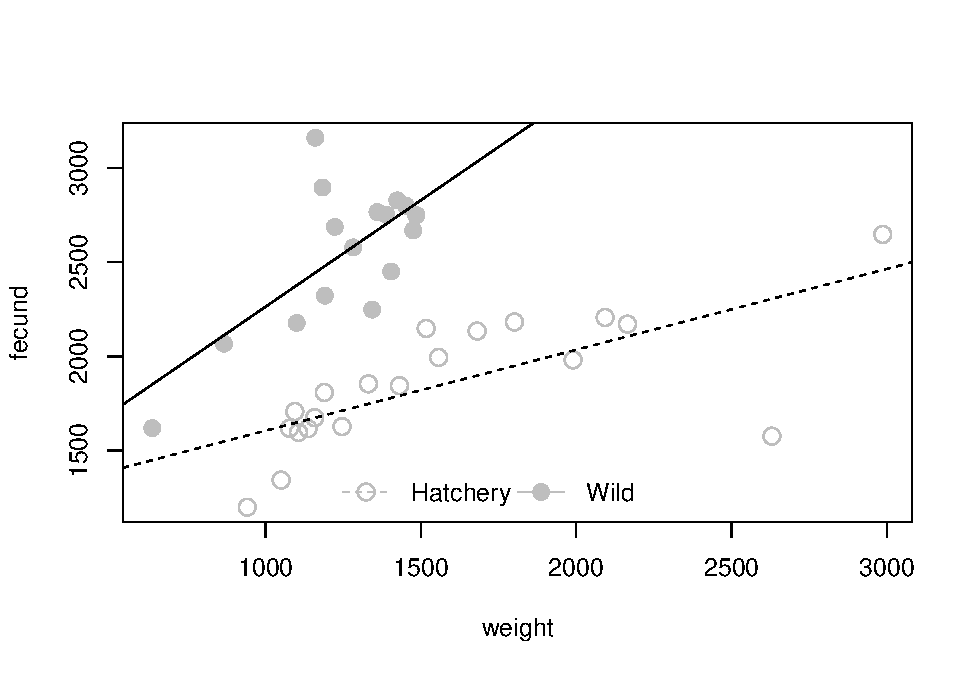
\includegraphics{au-r-workshop_files/figure-latex/unnamed-chunk-120-1} \end{center}

Fit another model comparing the success rates between hatchery and wild
fish:

\begin{Shaded}
\begin{Highlighting}[]
\NormalTok{fit2 =}\StringTok{ }\KeywordTok{glm}\NormalTok{(binary }\OperatorTok{~}\StringTok{ }\NormalTok{type, }\DataTypeTok{data =}\NormalTok{ dat, }\DataTypeTok{family =}\NormalTok{ binomial)}
\KeywordTok{summary}\NormalTok{(fit2)}\OperatorTok{$}\NormalTok{coef}
\end{Highlighting}
\end{Shaded}

\begin{verbatim}
##               Estimate Std. Error    z value  Pr(>|z|)
## (Intercept) -0.2006707  0.4494666 -0.4464641 0.6552620
## typewild     1.3793257  0.7272845  1.8965421 0.0578884
\end{verbatim}

An easier way to obtain the predicted probability is by using the
\texttt{predict} function:

\begin{Shaded}
\begin{Highlighting}[]
\KeywordTok{predict}\NormalTok{(fit2,}
        \DataTypeTok{newdata =} \KeywordTok{data.frame}\NormalTok{(}\DataTypeTok{type =} \KeywordTok{c}\NormalTok{(}\StringTok{"hatch"}\NormalTok{, }\StringTok{"wild"}\NormalTok{)),}
        \DataTypeTok{type =} \StringTok{"response"}\NormalTok{)}
\end{Highlighting}
\end{Shaded}

\begin{verbatim}
##         1         2 
## 0.4500000 0.7647059
\end{verbatim}

This plugs in the two possible values of the predictor variable and asks
for the fitted probabilities.

Incorporate the origin type into your original model:

\begin{Shaded}
\begin{Highlighting}[]
\NormalTok{fit3 =}\StringTok{ }\KeywordTok{glm}\NormalTok{(binary }\OperatorTok{~}\StringTok{ }\NormalTok{type }\OperatorTok{+}\StringTok{ }\NormalTok{weight, }\DataTypeTok{data =}\NormalTok{ dat)}
\end{Highlighting}
\end{Shaded}

and obtain/plot the fitted probabilities for each group:

\begin{Shaded}
\begin{Highlighting}[]
\NormalTok{p_hatch =}\StringTok{ }\KeywordTok{predict}\NormalTok{(}
\NormalTok{  fit3, }\DataTypeTok{newdata =} \KeywordTok{data.frame}\NormalTok{(}\DataTypeTok{type =} \StringTok{"hatch"}\NormalTok{, }\DataTypeTok{weight =}\NormalTok{ wt_seq),}
  \DataTypeTok{type =} \StringTok{"response"}
\NormalTok{)}
\NormalTok{p_wild =}\StringTok{ }\KeywordTok{predict}\NormalTok{(}
\NormalTok{  fit3, }\DataTypeTok{newdata =} \KeywordTok{data.frame}\NormalTok{(}\DataTypeTok{type =} \StringTok{"wild"}\NormalTok{, }\DataTypeTok{weight =}\NormalTok{ wt_seq),}
  \DataTypeTok{type =} \StringTok{"response"}
\NormalTok{)}

\KeywordTok{plot}\NormalTok{(p_wild }\OperatorTok{~}\StringTok{ }\NormalTok{wt_seq, }\DataTypeTok{type =} \StringTok{"l"}\NormalTok{, }\DataTypeTok{lwd =} \DecValTok{3}\NormalTok{, }\DataTypeTok{lty =} \DecValTok{1}\NormalTok{,}
     \DataTypeTok{ylim =} \KeywordTok{c}\NormalTok{(}\DecValTok{0}\NormalTok{,}\DecValTok{1}\NormalTok{), }\DataTypeTok{las =}\DecValTok{1}\NormalTok{,}
     \DataTypeTok{xlab =} \StringTok{"Weight (g)"}\NormalTok{, }\DataTypeTok{ylab =} \StringTok{"Pr(>70% Egg Survival)"}
\NormalTok{     )}
\KeywordTok{lines}\NormalTok{(p_hatch }\OperatorTok{~}\StringTok{ }\NormalTok{wt_seq, }\DataTypeTok{lwd =} \DecValTok{3}\NormalTok{, }\DataTypeTok{lty =} \DecValTok{2}\NormalTok{)}
\KeywordTok{legend}\NormalTok{(}\StringTok{"topright"}\NormalTok{, }\DataTypeTok{legend =} \KeywordTok{c}\NormalTok{(}\StringTok{"Hatchery"}\NormalTok{, }\StringTok{"Wild"}\NormalTok{),}
       \DataTypeTok{lty =} \KeywordTok{c}\NormalTok{(}\DecValTok{2}\NormalTok{,}\DecValTok{1}\NormalTok{), }\DataTypeTok{lwd =} \DecValTok{3}\NormalTok{, }\DataTypeTok{bty =} \StringTok{"n"}\NormalTok{)}
\end{Highlighting}
\end{Shaded}

\begin{center}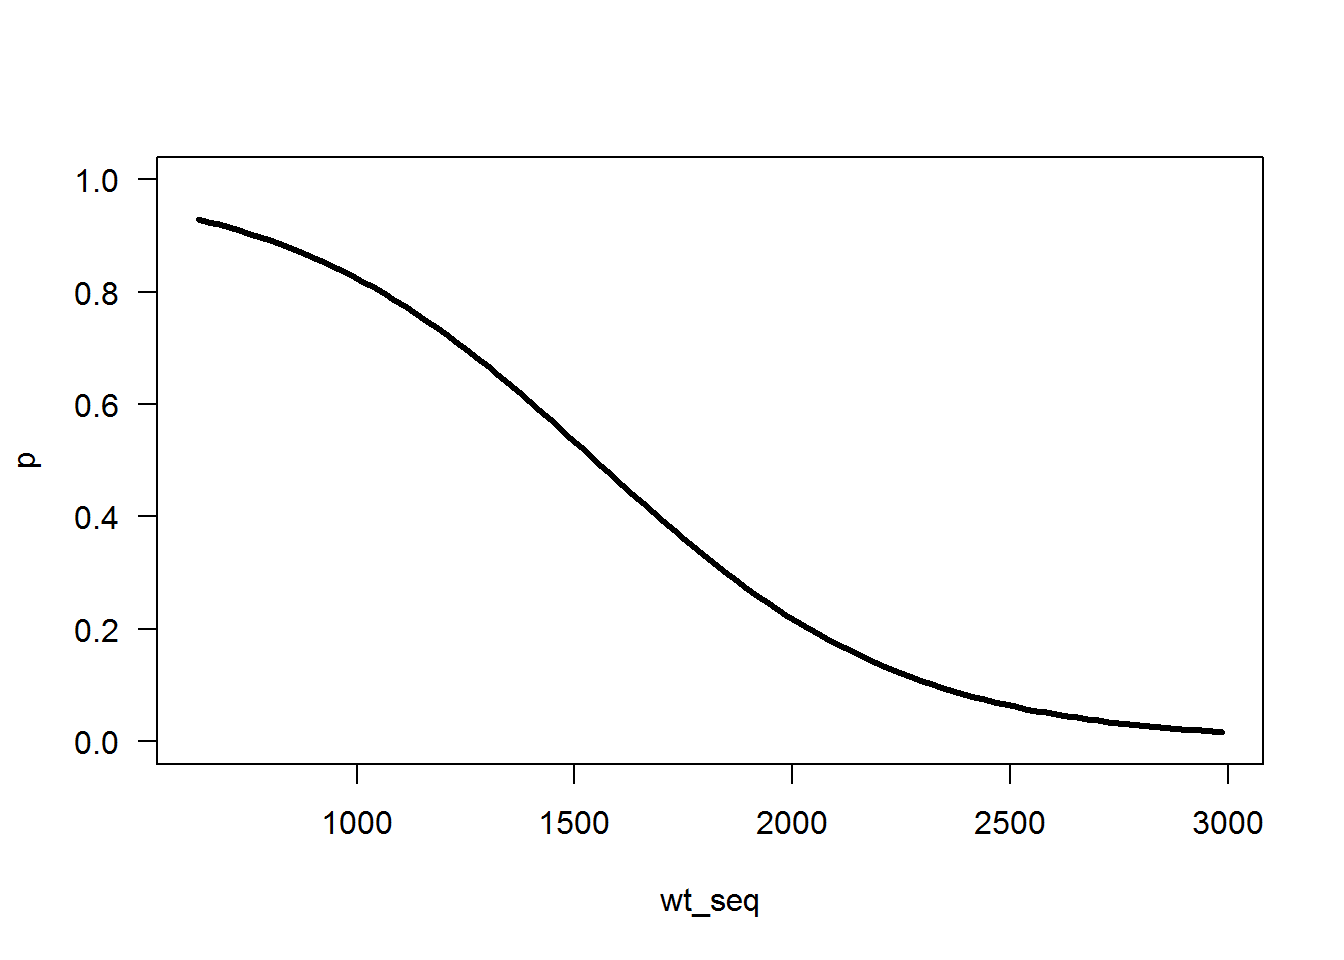
\includegraphics{au-r-workshop_files/figure-latex/unnamed-chunk-124-1} \end{center}

Look for an interaction (all the code is the same except use
\texttt{glm(binary\ \textasciitilde{}\ type\ *\ weight)} instead of
\texttt{glm(binary\ \textasciitilde{}\ type\ +\ weight)} and change
everything to \texttt{fit4} instead of \texttt{fit3}).

\begin{center}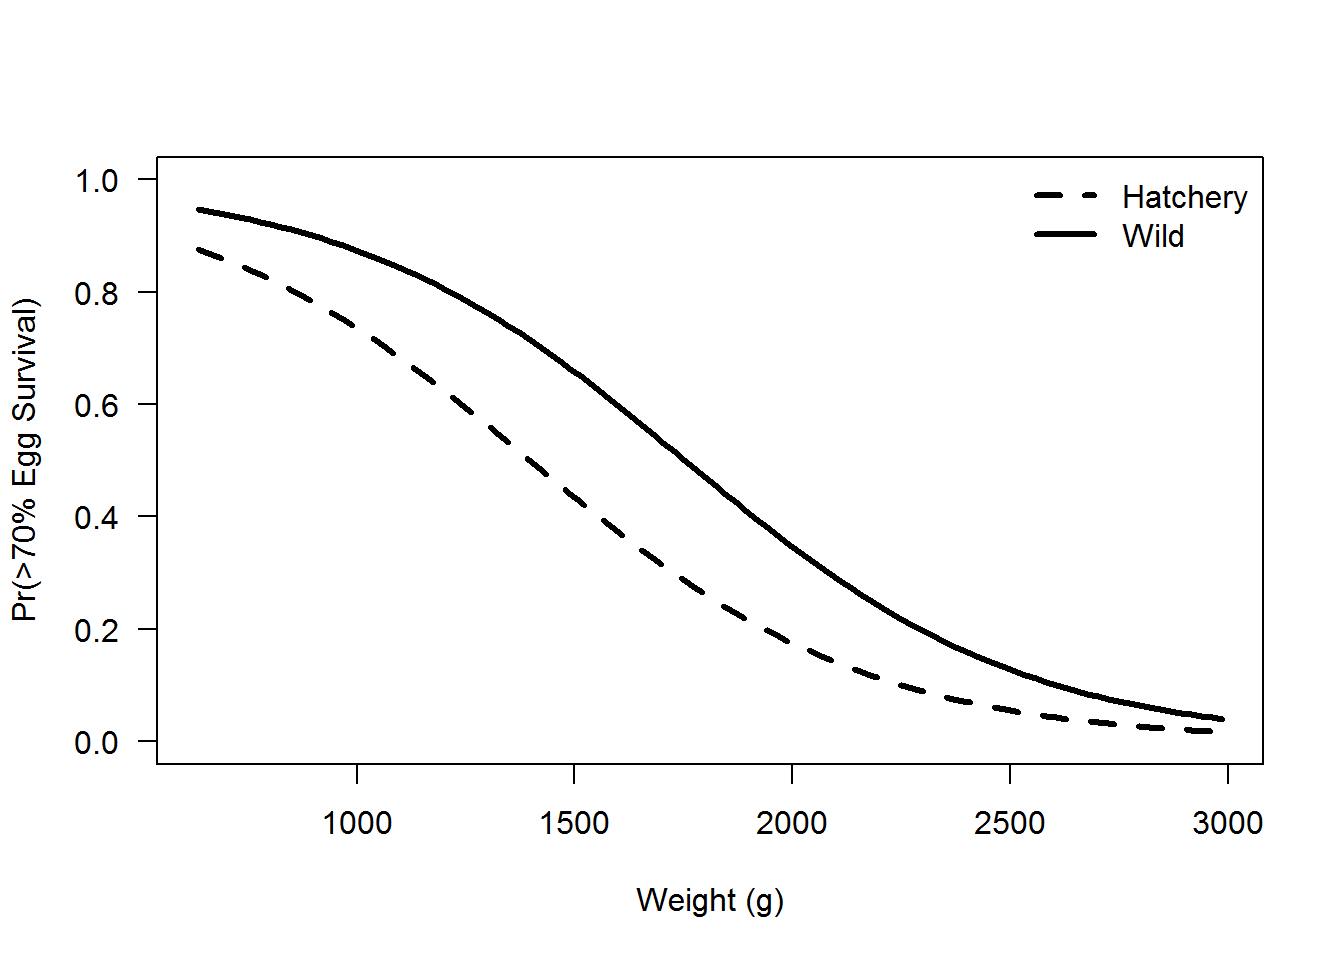
\includegraphics{au-r-workshop_files/figure-latex/unnamed-chunk-125-1} \end{center}

You may have noticed that you just did the same analysis with
\texttt{binary} as the response instead of \texttt{fecund}. Perform an
AIC analysis to determine which model is likely to be best for
prediction:

\begin{Shaded}
\begin{Highlighting}[]
\KeywordTok{AIC}\NormalTok{(fit1, fit2, fit3, fit4)}
\end{Highlighting}
\end{Shaded}

\begin{verbatim}
##      df      AIC
## fit1  2 45.40720
## fit2  2 50.07577
## fit3  4 50.42090
## fit4  3 46.00622
\end{verbatim}

Oddly enough, the two best models are the simplest one and the most
complex one, with \texttt{fit1} being the best, but not by a large
margin.

\section{Probability Distributions}\label{probability-distributions}

A probability distribution is a way of representing the probability of
an event or value of a parameter and they are central to statistical
theory. Some of the most commonly used distributions are summarized in
Table \ref{tab:dist-table} below, along with the suffixes of the
functions in R that correspond to each distribution\footnote{For an
  excellent and ecologically-focused description of probability
  distributions, checkout Ben Bolker's book, \emph{Ecological Models and
  Data in R}. There is a free proof version online:
  \url{https://ms.mcmaster.ca/~bolker/emdbook/book.pdf}}.

\begin{table}

\caption{\label{tab:dist-table}A brief description of probability distributions commonly used in ecological problems, including the function suffix in R.}
\centering
\begin{tabular}[t]{lll|lll|lll|lll}
\hline
Type & Distribution & Common Uses & R Suffix\\
\hline
Continuous & Normal & Models the relative frequency of outcomes that are symmetric around a mean, can be negative & `-norm`\\
\hline
 & Lognormal & Models the relative frequency of outcomes that are normally-distributed on the log-scale & `-lnorm`\\
\hline
 & Uniform & Models values that are between two endpoints and that all occur with the same frequency & `-unif`\\
\hline
 & Beta & Models values that are between 0 and 1 & `-beta`\\
\hline
Discrete & Binomial & Models the number of successes from a given number of trials when there are only two possible outcomes and all trials have the same probability of success & `-binom`\\
\hline
 & Multinomial & The same as the binomial distribution, but when there are more than two possible outcomes & `-multinom`\\
\hline
 & Poisson & Used for count data in cases where the variance and mean are roughly equal & `-pois`\\
\hline
\end{tabular}
\end{table}

In R, there are four different ways to use each of this distribution
functions (each as a separate prefix):

\begin{itemize}
\item
  \textbf{The probability density (or mass) function} (\texttt{d-}): the
  height of the probability distribution function at some given value of
  the random variable.
\item
  \textbf{The cumulative density function} (\texttt{p-}): the sum of the
  probability densities for all random variables below some value.
\item
  \textbf{The quantile function} (\texttt{-q}): what value of the random
  variable do p\% fall below?
\item
  \textbf{The random deviates function} (\texttt{-r}): generates random
  variables from the distribution in proportion to their probability
  density.
\end{itemize}

Suppose that \(x\) represents the length of individual age 6 largemouth
bass in your private fishing pond. Assume that
\(x \sim N(\mu=500, \sigma=50)\) (\(x\) is a normal random variable with
mean equal to 500 and standard deviation equal to 50). Here is the usage
of each of the distribution functions and a plot illustrating them:

\begin{Shaded}
\begin{Highlighting}[]
\CommentTok{# parameters}
\NormalTok{mu =}\StringTok{ }\DecValTok{500}\NormalTok{; sig =}\StringTok{ }\DecValTok{50}

\CommentTok{# a sequence of possible random variables (fish lengths)}
\NormalTok{lengths =}\StringTok{ }\KeywordTok{seq}\NormalTok{(}\DecValTok{200}\NormalTok{, }\DecValTok{700}\NormalTok{, }\DataTypeTok{length =} \DecValTok{100}\NormalTok{)}

\CommentTok{# a sequence of possible cumulative probabilities}
\NormalTok{cprobs =}\StringTok{ }\KeywordTok{seq}\NormalTok{(}\DecValTok{0}\NormalTok{, }\DecValTok{1}\NormalTok{, }\DataTypeTok{length =} \DecValTok{100}\NormalTok{)}

\NormalTok{densty =}\StringTok{ }\KeywordTok{dnorm}\NormalTok{(}\DataTypeTok{x =}\NormalTok{ lengths, }\DataTypeTok{mean =}\NormalTok{ mu, }\DataTypeTok{sd =}\NormalTok{ sig)  }\CommentTok{# takes specific lengths}
\NormalTok{cuprob =}\StringTok{ }\KeywordTok{pnorm}\NormalTok{(}\DataTypeTok{q =}\NormalTok{ lengths, }\DataTypeTok{mean =}\NormalTok{ mu, }\DataTypeTok{sd =}\NormalTok{ sig)  }\CommentTok{# takes specific lengths}
\NormalTok{quants =}\StringTok{ }\KeywordTok{qnorm}\NormalTok{(}\DataTypeTok{p =}\NormalTok{ cprobs, }\DataTypeTok{mean =}\NormalTok{ mu, }\DataTypeTok{sd =}\NormalTok{ sig)   }\CommentTok{# takes specific probabilities}
\NormalTok{random =}\StringTok{ }\KeywordTok{rnorm}\NormalTok{(}\DataTypeTok{n =} \FloatTok{1e4}\NormalTok{, }\DataTypeTok{mean =}\NormalTok{ mu, }\DataTypeTok{sd =}\NormalTok{ sig)      }\CommentTok{# takes a number of random deviates to make}

\CommentTok{# set up plotting region: see ?par for more details}
\CommentTok{# notice the tricks to clean up the plot}
\KeywordTok{par}\NormalTok{(}
  \DataTypeTok{mfrow =} \KeywordTok{c}\NormalTok{(}\DecValTok{2}\NormalTok{,}\DecValTok{2}\NormalTok{),    }\CommentTok{# set up 2x2 regions}
  \DataTypeTok{mar =} \KeywordTok{c}\NormalTok{(}\DecValTok{3}\NormalTok{,}\DecValTok{3}\NormalTok{,}\DecValTok{3}\NormalTok{,}\DecValTok{1}\NormalTok{),  }\CommentTok{# set narrower margins}
  \DataTypeTok{xaxs =} \StringTok{"i"}\NormalTok{,        }\CommentTok{# remove "x-buffer"}
  \DataTypeTok{yaxs =} \StringTok{"i"}\NormalTok{,        }\CommentTok{# remove "y-buffer"}
  \DataTypeTok{mgp =} \KeywordTok{c}\NormalTok{(}\DecValTok{2}\NormalTok{,}\FloatTok{0.4}\NormalTok{,}\DecValTok{0}\NormalTok{),  }\CommentTok{# bring in axis titles ([1]) and tick labels ([2])}
  \DataTypeTok{tcl =} \OperatorTok{-}\FloatTok{0.25}        \CommentTok{# shorten tick marks}
\NormalTok{)}

\KeywordTok{plot}\NormalTok{(densty }\OperatorTok{~}\StringTok{ }\NormalTok{lengths, }\DataTypeTok{type =} \StringTok{"l"}\NormalTok{, }\DataTypeTok{lwd =} \DecValTok{3}\NormalTok{, }\DataTypeTok{main =} \StringTok{"dnorm()"}\NormalTok{,}
     \DataTypeTok{xlab =} \StringTok{"Fish Length (mm)"}\NormalTok{, }\DataTypeTok{ylab =} \StringTok{"Density"}\NormalTok{, }\DataTypeTok{las =} \DecValTok{1}\NormalTok{,}
     \DataTypeTok{yaxt =} \StringTok{"n"}\NormalTok{) }\CommentTok{# turns off y-axis}
\KeywordTok{axis}\NormalTok{(}\DataTypeTok{side =} \DecValTok{2}\NormalTok{, }\DataTypeTok{at =} \KeywordTok{c}\NormalTok{(}\FloatTok{0.002}\NormalTok{, }\FloatTok{0.006}\NormalTok{), }\DataTypeTok{labels =} \KeywordTok{c}\NormalTok{(}\FloatTok{0.002}\NormalTok{, }\FloatTok{0.006}\NormalTok{), }\DataTypeTok{las =} \DecValTok{2}\NormalTok{)}
\KeywordTok{plot}\NormalTok{(cuprob }\OperatorTok{~}\StringTok{ }\NormalTok{lengths, }\DataTypeTok{type =} \StringTok{"l"}\NormalTok{, }\DataTypeTok{lwd =} \DecValTok{3}\NormalTok{, }\DataTypeTok{main =} \StringTok{"pnorm()"}\NormalTok{,}
     \DataTypeTok{xlab =} \StringTok{"Fish Length (mm)"}\NormalTok{, }\DataTypeTok{ylab =} \StringTok{"Cumulative Probability"}\NormalTok{, }\DataTypeTok{las =} \DecValTok{1}\NormalTok{)}
\KeywordTok{plot}\NormalTok{(quants }\OperatorTok{~}\StringTok{ }\NormalTok{cprobs, }\DataTypeTok{type =} \StringTok{"l"}\NormalTok{, }\DataTypeTok{lwd =} \DecValTok{3}\NormalTok{, }\DataTypeTok{main =} \StringTok{"qnorm()"}\NormalTok{,}
     \DataTypeTok{xlab =} \StringTok{"P"}\NormalTok{, }\DataTypeTok{ylab =} \StringTok{"P Quantile Length (mm)"}\NormalTok{, }\DataTypeTok{las =} \DecValTok{1}\NormalTok{)}
\KeywordTok{hist}\NormalTok{(random, }\DataTypeTok{breaks =} \DecValTok{100}\NormalTok{, }\DataTypeTok{col =} \StringTok{"grey"}\NormalTok{, }\DataTypeTok{main =} \StringTok{"rnorm()"}\NormalTok{,}
     \DataTypeTok{xlab =} \StringTok{"Fish Length (mm)"}\NormalTok{, }\DataTypeTok{ylab =} \StringTok{"Frequency"}\NormalTok{, }\DataTypeTok{las =} \DecValTok{1}\NormalTok{)}
\KeywordTok{box}\NormalTok{() }\CommentTok{# add borders to the histogram}
\end{Highlighting}
\end{Shaded}

\begin{figure}

{\centering 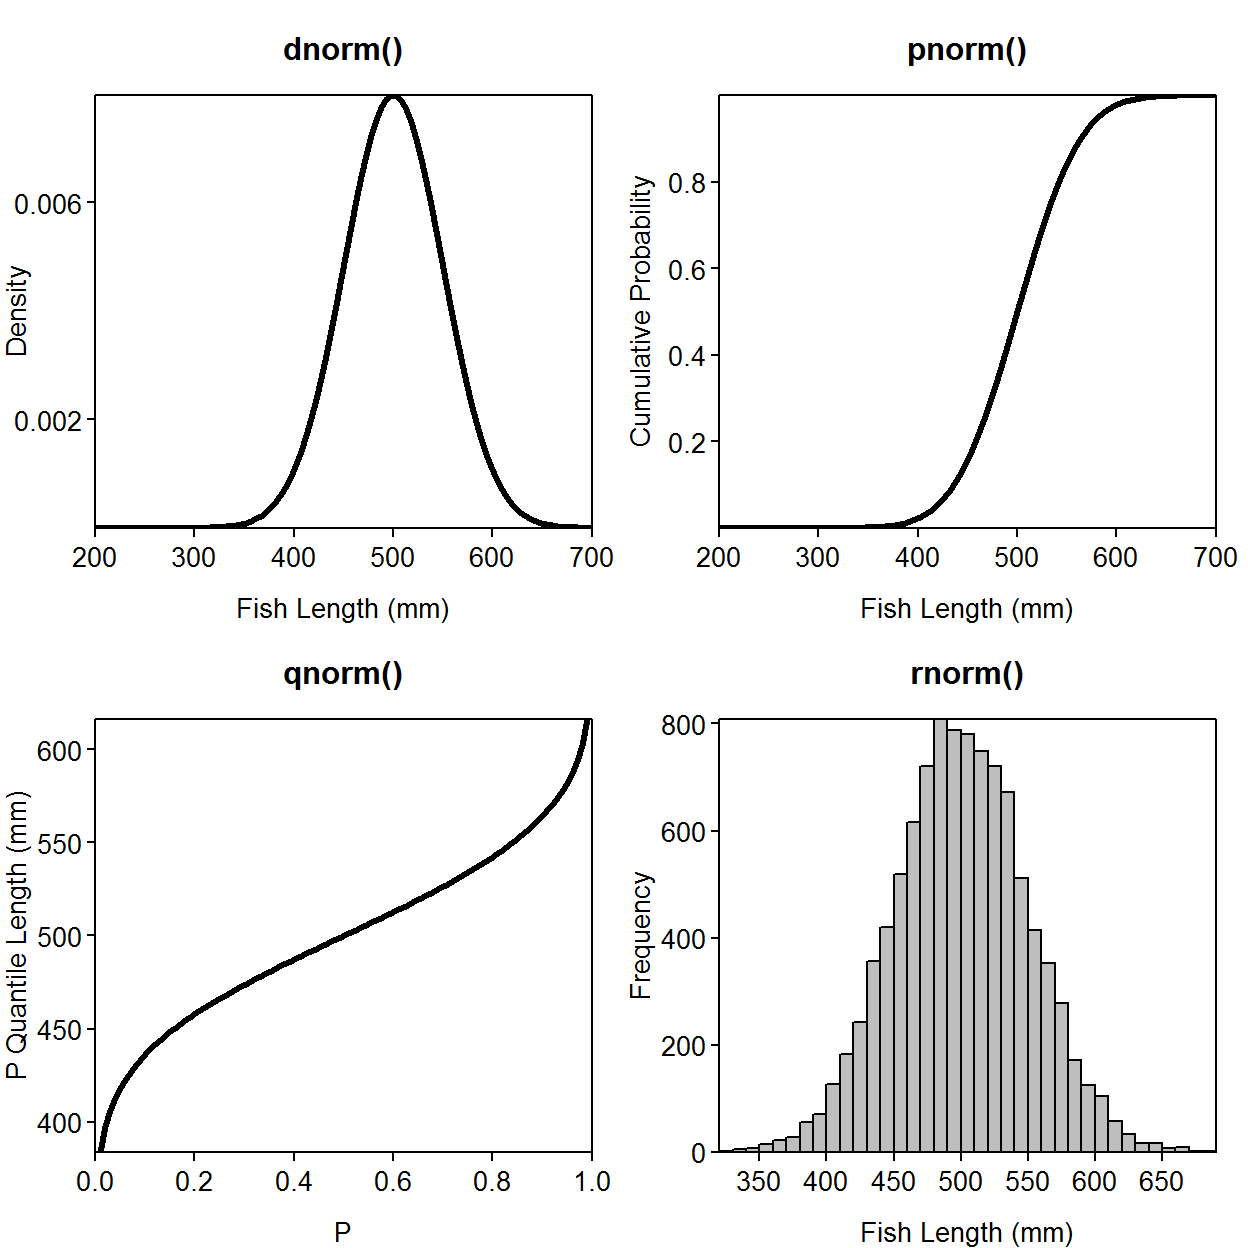
\includegraphics{au-r-workshop_files/figure-latex/norm-plots-1} 

}

\caption{The four `-norm` functions with input (x-axis) and output (y-axis) displayed.}\label{fig:norm-plots}
\end{figure}

Notice that \texttt{pnorm} and \texttt{qnorm} are inverses of one
another: if you put the output of one into the output of the other, you
get the original input back:

\begin{Shaded}
\begin{Highlighting}[]
\KeywordTok{qnorm}\NormalTok{(}\KeywordTok{pnorm}\NormalTok{(}\DecValTok{0}\NormalTok{))}
\end{Highlighting}
\end{Shaded}

\begin{verbatim}
## [1] 0
\end{verbatim}

\texttt{pnorm(0)} asks R to find the probability that \(x\) is less than
zero for the standard normal distribution (\(N(0,1)\) - this is the
default if you don't specify \texttt{mean} and \texttt{sig}).
\texttt{qnorm(pnorm(0))} asks R to find the value of \(x\) that
\texttt{pnorm(0)} * 100\% of the possible values fall below. If the
nesting is confusing, this line is the same as:

\begin{Shaded}
\begin{Highlighting}[]
\NormalTok{p =}\StringTok{ }\KeywordTok{pnorm}\NormalTok{(}\DecValTok{0}\NormalTok{)}
\KeywordTok{qnorm}\NormalTok{(p)}
\end{Highlighting}
\end{Shaded}

\section{Bonus Topic: Non-linear
Regression}\label{bonus-topic-non-linear-regression}

You fitted linear and logistic regression models in Sections
\ref{regression} and \ref{logis-regression}, however, R allows you to
fit non-linear regression models as well.

First, aquire the \texttt{feeding.csv} data set from the
\href{https://www.github.com/bstaton1/au-r-workshop-data}{GitHub repo}
and place it in your working directory. Read the data into R:

\begin{verbatim}
##       prey            cons      
##  Min.   : 1.00   Min.   : 1.00  
##  1st Qu.:11.25   1st Qu.: 8.00  
##  Median :26.00   Median :11.00  
##  Mean   :25.08   Mean   : 9.92  
##  3rd Qu.:37.75   3rd Qu.:13.00  
##  Max.   :49.00   Max.   :15.00
\end{verbatim}

\begin{Shaded}
\begin{Highlighting}[]
\NormalTok{dat =}\StringTok{ }\KeywordTok{read.csv}\NormalTok{(}\StringTok{"feeding.csv"}\NormalTok{); }\KeywordTok{summary}\NormalTok{(dat)}
\end{Highlighting}
\end{Shaded}

These are hypothetical data from an experiment in which you were
interested in quantifying the functional feeding response\footnote{A
  functional response is the number of prey consumed by a predator at
  various prey densities} of a fish predator on zooplankton in an
aquarium. You experimentally manipulated the prey density
(\texttt{dat\$prey}) and counted how many prey items were consumed
(\texttt{dat\$cons}).

Plot the data:

\begin{Shaded}
\begin{Highlighting}[]
\KeywordTok{plot}\NormalTok{(cons }\OperatorTok{~}\StringTok{ }\NormalTok{prey, }\DataTypeTok{data =}\NormalTok{ dat)}
\end{Highlighting}
\end{Shaded}

\begin{center}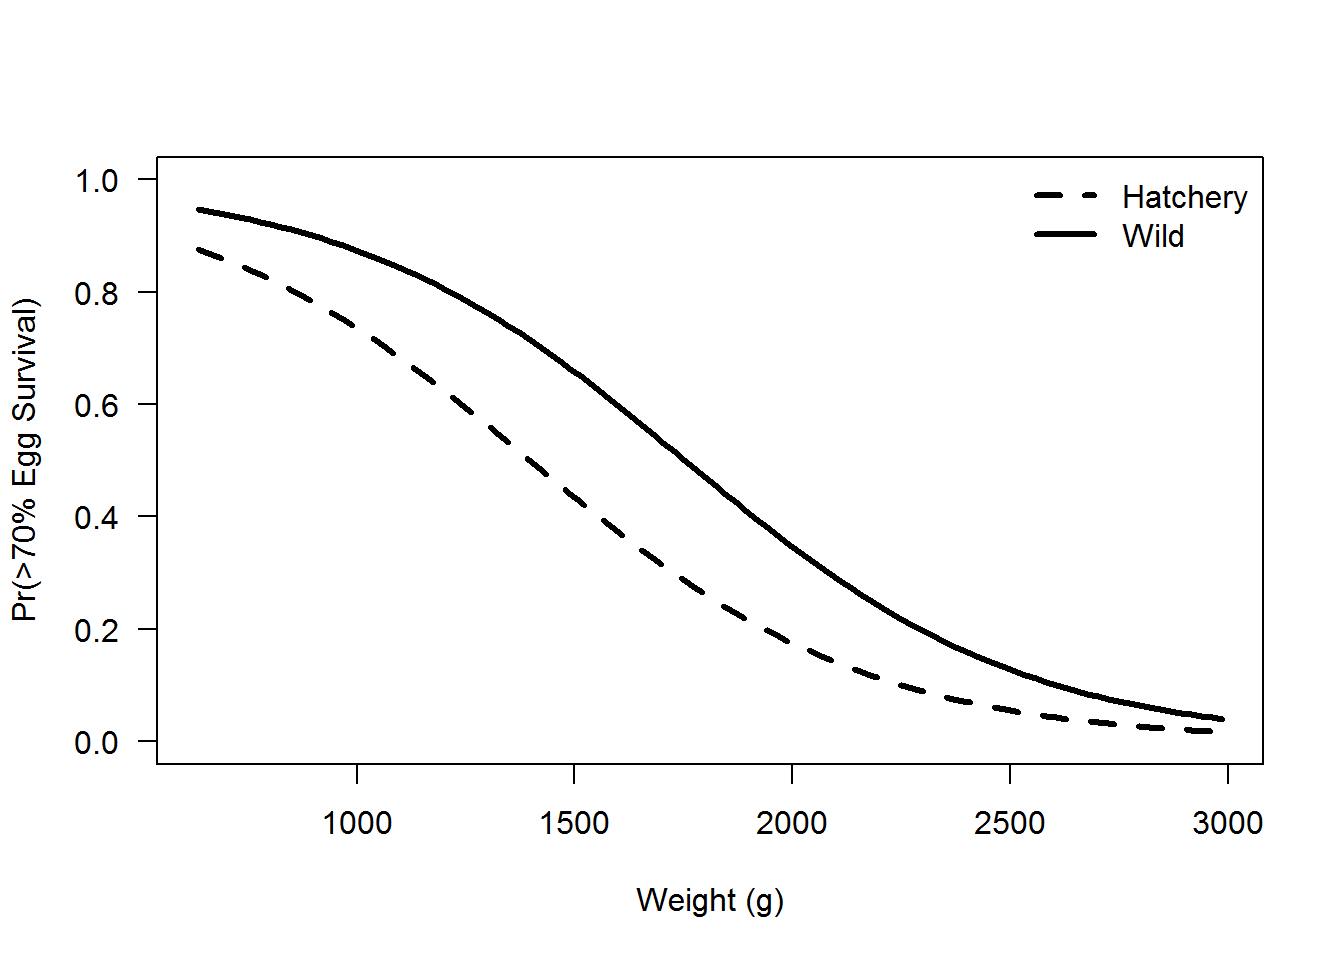
\includegraphics{au-r-workshop_files/figure-latex/unnamed-chunk-131-1} \end{center}

You can see a distinct non-linearity to the relationship. The Holling
Type II functional response\footnote{This function rises quickly at low
  prey densities, but saturates at high densities} has this functional
form:

\[y_i=\frac{ax_i}{1+ahx_i}\] where \(x_i\) is \texttt{prey} and \(y_i\)
is \texttt{cons}.

You can fit this model in R using the \texttt{nls} function, behaves
very similarly to the \texttt{lm} function.

\begin{Shaded}
\begin{Highlighting}[]
\NormalTok{fit =}\StringTok{ }\KeywordTok{nls}\NormalTok{(cons }\OperatorTok{~}\StringTok{ }\NormalTok{(a }\OperatorTok{*}\StringTok{ }\NormalTok{prey)}\OperatorTok{/}\NormalTok{(}\DecValTok{1} \OperatorTok{+}\StringTok{ }\NormalTok{a }\OperatorTok{*}\StringTok{ }\NormalTok{h }\OperatorTok{*}\StringTok{ }\NormalTok{prey), }\DataTypeTok{data =}\NormalTok{ dat,}
          \DataTypeTok{start =} \KeywordTok{c}\NormalTok{(}\DataTypeTok{a =} \DecValTok{3}\NormalTok{, }\DataTypeTok{h =} \FloatTok{0.1}\NormalTok{))}
\end{Highlighting}
\end{Shaded}

You can obtain similar output as from \texttt{lm} using the
\texttt{summary}, \texttt{coef}, and \texttt{predict}. Draw the fitted
line over top of the data:

\begin{Shaded}
\begin{Highlighting}[]
\NormalTok{prey_seq =}\StringTok{ }\KeywordTok{seq}\NormalTok{(}\KeywordTok{min}\NormalTok{(dat}\OperatorTok{$}\NormalTok{prey), }\KeywordTok{max}\NormalTok{(dat}\OperatorTok{$}\NormalTok{prey), }\DataTypeTok{length =} \DecValTok{100}\NormalTok{)}
\NormalTok{cons_seq =}\StringTok{ }\KeywordTok{predict}\NormalTok{(fit, }\DataTypeTok{newdata =} \KeywordTok{data.frame}\NormalTok{(}\DataTypeTok{prey =}\NormalTok{ prey_seq))}

\KeywordTok{plot}\NormalTok{(cons }\OperatorTok{~}\StringTok{ }\NormalTok{prey, }\DataTypeTok{data =}\NormalTok{ dat, }\DataTypeTok{cex =} \FloatTok{1.5}\NormalTok{, }\DataTypeTok{pch =} \DecValTok{16}\NormalTok{, }\DataTypeTok{col =} \StringTok{"grey"}\NormalTok{)}
\KeywordTok{lines}\NormalTok{(cons_seq }\OperatorTok{~}\StringTok{ }\NormalTok{prey_seq, }\DataTypeTok{lwd =} \DecValTok{3}\NormalTok{)}
\end{Highlighting}
\end{Shaded}

\begin{center}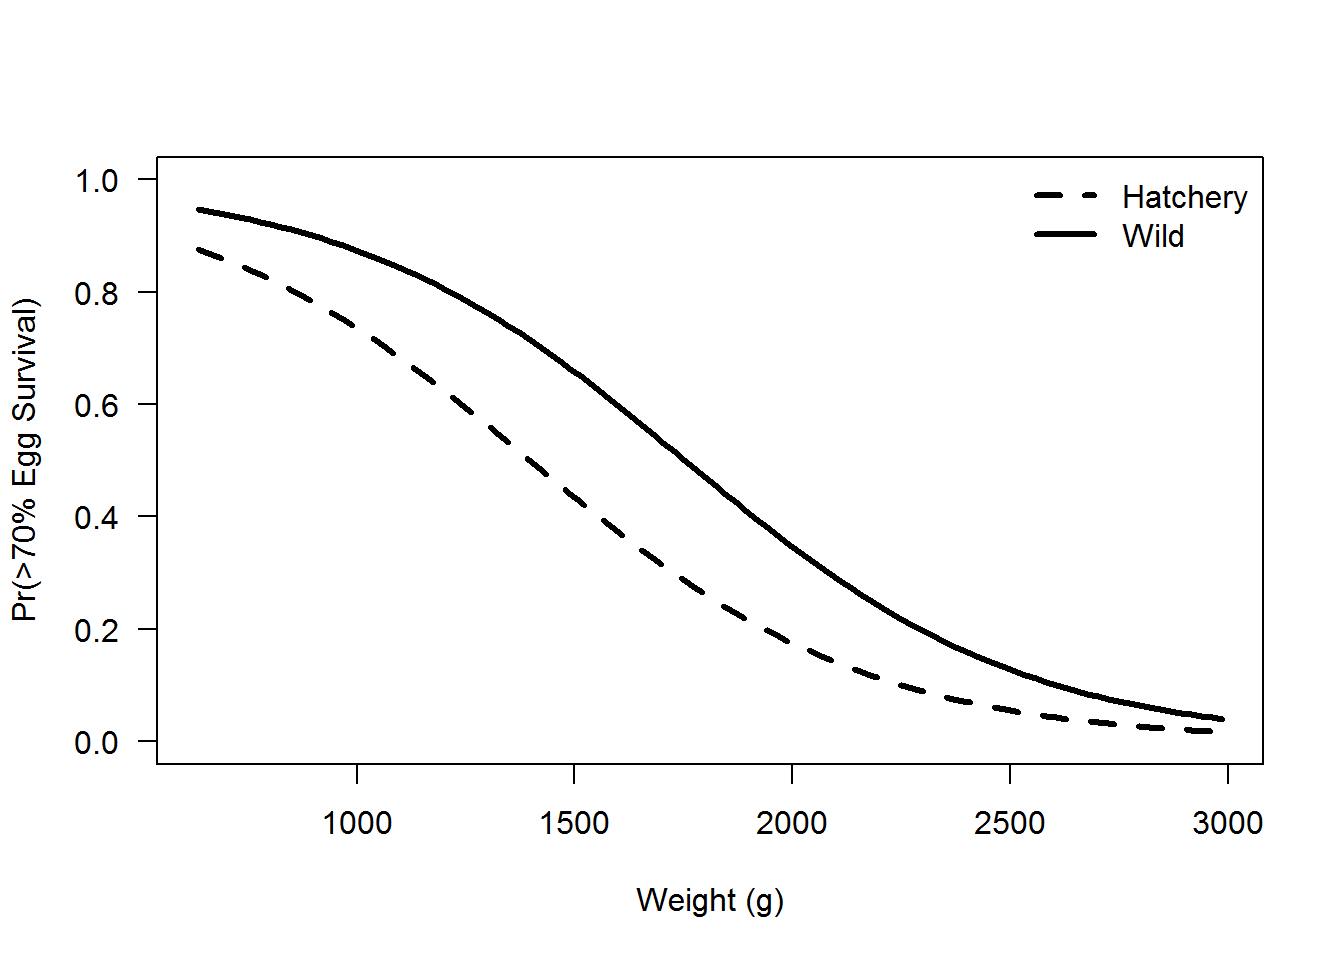
\includegraphics{au-r-workshop_files/figure-latex/unnamed-chunk-133-1} \end{center}

\section*{EXERCISE 3}\label{exercise-3}
\addcontentsline{toc}{section}{EXERCISE 3}

\begin{enumerate}
\def\labelenumi{\arabic{enumi}.}
\tightlist
\item
  Make the same graphic as in Figure \ref{fig:norm-plots} with at least
  one of the other distributions listed in Table \ref{tab:dist-table}
  (other than the multinomial - being a multivariate distribution, it
  wouldn't work well with this code). Try thinking of a variable from
  your work that meets the uses of each distribution in Table
  \ref{tab:dist-table} (or one that's not listed). If you run into
  trouble, check out the help file for that distribution\footnote{Executing
    \texttt{?rnorm} or any other of the \texttt{-norm} functions will
    take you to a page with info on all four function types for that
    distribution}.
\end{enumerate}

\chapter{Simulation and Randomization}\label{ch4}

\chapter{Large Data Manipulation}\label{ch5}

\bibliography{book.bib,packages.bib}


\end{document}
